\chapter{Dynamics Modelling}

In this chapter, we
present the mathematical forumulation of the orbit and attitude dynamcis models in GMAT.
One of the fundamental capabilities of GMAT is to model the motion
of spacecraft in different flight regimes.  The flight regime,
such as low Earth, libration point, or lunar, are determined by the
forces and perturbations that dominate the dynamics.
The chapter begins with an overview of
the orbital equations of motion and their variational equations.  Next, we
discuss the formulation for orbital perturbations and the equations used to model
spacecraft thrust.  The second half of the chapter is devoted to attitude modeling and
we present the specifications for  attitude conversions and kinematic attitude models.


\section{Orbit Dynamics}

\subsection{Orbital Equations of Motion}

The orbital equations of motion come from an application of Newton's laws of motion to a spacecraft in orbit.  From Newton's Second Law we know that
%
\begin{equation}
     \frac{d (m\mathbf{v})}{d t} = \sum F_{ext}
\end{equation}
%
where $m$ is the total mass of the spacecraft, $\mathbf{r}$ is the position vector of the spacecraft, $t$ is time, and the right hand side of the equation represents the total sum of external forces.  Solving for the acceleration gives us the
second order differential equation
%
\begin{equation}
   \frac{d^2 \mathbf{r}}{d^2 t} = \sum \frac{F_{ext}}{m} - \frac{\dot{m}}{m}\frac{\partial \mathbf{r}}{\partial t}
   \label{Eq:SCAcc}
\end{equation}
%

The terms included in the RHS of the equations of motion can be selected by the user, and the form of several terms (and whether they appear at all) are dependent upon the coordinate system of integration.    If we include
all of the possible forces GMAT can model in the summation on the
RHS of Eq.~(\ref{Eq:SCAcc}), and we assume the origin of integration is a celestial body (the barycentric form is slightly different), then the orbital equations of motion are
%
\begin{equation} \begin{split}
    \frac{d^2\mathbf{r}}{dt^2}
    =  &-\frac{\mu}{r^3}\mathbf{r} +  \nabla \phi_{sj}^o +
    %
    G\sum_{\stackrel{k=1}{k \neq j}}^{n_b}m_k \left(\frac{\mathbf{r}_{ks}}{r_{ks}^3} -
     \frac{\mathbf{r}_{kj} }{r_{kj}^3}   \right)
     %
    + %\sum_{\stackrel{k=1}{k \neq j}}^{n_b}\left( \nabla
    %\phi_{ks}^o +
     %\nabla\phi_{kj}^o
     %\right)+
     \frac{\dot{m}_s }{m}\frac{d\mathbf{r}}{dt}- \frac{1}{2}\rho v_{rel}^2 \frac{C_d A}{m_s}\hat{\mathbf{v}}_{rel}
     +\frac{   P_{SR}C_R A_{\odot}   }{m_s}\hat{\mathbf{r}}_{s\odot} + \\ &
         \frac{\mu}{c^2 r^3}\left(  \left( 4\frac{\mu}{r} - v^2\right)\mathbf{r} +   4(\mathbf{r}\cdot\mathbf{v})\mathbf{v}\right) + 2 (\boldsymbol{\Omega} \times \mathbf{v}) + 2 \frac{\mu}{c^2 r^3}
    \left( \frac{3}{r^2}(\mathbf{r} \times \mathbf{v})(\mathbf{r} \cdot \mathbf{J}) +(\mathbf{v}\times\mathbf{J}) \right)
     \label{Eq:CompleteEOM}
     \end{split}
\end{equation}
%
Table \ref{Eq:AllForces} below describes each force in the equation above.
%
\begin{table}[h]
\centering \caption{ Force Models Available in GMAT } \label{Eq:AllForces}
\begin{tabular}{p{2.0 in} p{2.75 in} }
  \hline\hline
  % after \\: \hline or \cline{col1-col2} \cline{col3-col4} ...
  Description & Term \\
  \hline
  Central Body Point Mass & $ -\displaystyle\frac{\mu}{r^3}\mathbf{r}$ \\
  & \\
  Central Body Direct Nonspherical &  $\nabla \phi_{sj}^o$  \\
  & \\
  Direct Third Body Point Mass & $G\displaystyle\sum_{\stackrel{k=1}{k \neq j}}^{n_b}m_k \left(\frac{\mathbf{r}_{ks}}{r_{ks}^3}\right)$ \\
   & \\
  Indirect Third Body Point Mass &  $G\displaystyle\sum_{\stackrel{k=1}{k \neq j}}^{n_b}m_k \left( -
     \frac{\mathbf{r}_{kj} }{r_{kj}^3}   \right)$ \\
      & \\
   %Third Body Direct Nonspherical & $\displaystyle\sum_{\stackrel{k=1}{k \neq j}}^{n_b}\left( \nabla
   % \phi_{ks}^o\right)$  \\
   % &\\
   % Third Body Indirect Nonspherical &  $\sum_{\stackrel{k=1}{k \neq j}}^{n_b}\left(
   %  \nabla\phi_{kj}^o \right)$\\
   % & \\
   Spacecraft Thrust &$\displaystyle\frac{\dot{m}_s }{m}\frac{d\mathbf{r}}{dt}$\\
   &\\
   Atmospheric Drag & $- \displaystyle\frac{1}{2}\rho v_{rel}^2 \displaystyle\frac{C_d
   A}{m_s}\hat{\mathbf{v}}_{rel}$\\
   &\\
   Solar Radiation Pressure & $\displaystyle\frac{   P_{SR}C_R A_{\odot}   }{m_s}\hat{\mathbf{r}}_{s\odot}$\\
   &\\
   Schwarzschild solution & $\displaystyle\frac{\mu}{c^2 r^3}\left(  \left( 4\frac{\mu}{r} - v^2\right)\mathbf{r} +            4(\mathbf{r}\cdot\mathbf{v})\mathbf{v}\right) + 2 (\boldsymbol{\Omega} \times \mathbf{v})$\\
      &\\
   Geodesic Precession & $2 (\boldsymbol{\Omega} \times \mathbf{v}) $\\
         &\\
   Lense-Thirring Precession & $2 \displaystyle\frac{\mu}{c^2 r^3}
    \left( \frac{3}{r^2}(\mathbf{r} \times \mathbf{v})(\mathbf{r} \cdot \mathbf{J}) +(\mathbf{v}\times\mathbf{J}) \right)$\\
  \hline\hline
\end{tabular}
\end{table}
%
\subsection{Coordinate Systems for Integration of the Equations of Motion}

\subsection{Orbit Variational Equations and the State Transition Matrix}

Estimation and optimization problems require first derivatives of the solution
to the orbit final value problem with respect to orbital initial conditions.  Those
derivatives are provided by the orbit variational equations.  The variatial equations are
obtained by expanding the orbital equations of motion in a Taylor series and retaining
only the linear terms.
%
Assume the nonlinear dynamics have the following form
%
\begin{equation}
    \dot{\mathbf{x}} = \mathbf{f}(\mathbf{x},t)
\end{equation}
%
where
%
\begin{equation}
    \mathbf{x} = \left[\mbr^T \hspace{.2 in} \mbv^T  \right]^T = \left[x \hspace{.2 in} y \hspace{.2 in} z \hspace{.2 in} \dot{x} \hspace{.2 in}
    \dot{y} \hspace{.2 in} \dot{z}  \right]^T
\end{equation}
%
and
%
\begin{equation}
    \dot{\mathbf{x}} = \left[\dot{\mbr}^T \hspace{.2 in} \dot{\mbv}^T  \right]^T = \left[\dot{x} \hspace{.2 in}
    \dot{y}
    \hspace{.2 in} \dot{z} \hspace{.2 in} \ddot{x} \hspace{.2 in}
    \ddot{y} \hspace{.2 in} \ddot{z}  \right]^T
\end{equation}
%
Expanding the dynamics equations and retaining only the first order terms yields
%
\begin{equation}
    \dot{\mathbf{x}} \approx  \dot{\mathbf{x}}|_{ref} + \frac{\partial \mathbf{f}}
    {\partial \mathbf{x}}\left( \mathbf{x} - \mathbf{x}|_{ref} \right)\label{Eq:VarTaylorSeries}
\end{equation}
%
%
We can rewrite Eq.~(\ref{Eq:VarTaylorSeries}) by defining $\delta \mathbf{x} = \dot{\mathbf{x}} - \dot{\mathbf{x}}|_{ref}$ as follows.
%
\begin{equation}
    \delta \dot{\mathbf{x}} = \mathbf{A}\delta \mathbf{x}\label{Eq:LinearizedOEM}
\end{equation}
%
where
%
the Jacobian of the state equations is defined as the ``A" matrix as follows:
%
\begin{equation}
    \mathbf{A} = \frac{\partial \mathbf{f}}{\partial \mathbf{x}}
\end{equation}

From linear systems theory, the solution to Eq.~(\ref{Eq:LinearizedOEM}) has the form
%
\begin{equation}
     \delta \mathbf{x}(t_f) = \boldsymbol{\Phi}(t,t_o)\delta \mathbf{x}(t_o)
\end{equation}
%
where $\dot{\boldsymbol{\Phi}}$ is governed by the following set of 36 differential equations:
%
\begin{equation}
     \dot{\boldsymbol{\Phi}} = \mathbf{A}\boldsymbol{\Phi}
\end{equation}
%
GMAT simultaneously integrates the variational equations along with the non-linear state equations from $t_o$ to $t_f$ to obtain the State Transition Matrix (STM):
%
\begin{equation}
     \boldsymbol{\Phi}(t_o,t_f) = \int_{t_o}^{t_f}\mathbf{A}\boldsymbol{\Phi} dt \label{Eq:STMSolution}
\end{equation}
%
subject to the initial conditions
%
\begin{equation}
     \boldsymbol{\Phi}(t_o,t_o) = \mathbf{I}_{6\times6}
\end{equation}
%
To perform the integration in Eq.~(\ref{Eq:STMSolution}) we require the partial derivatives contained in the matrix $\mathbf{A}$:
%
\begin{equation}
     \mathbf{A} = \frac{\partial \dot{\mathbf{x}}}{\partial
     \mathbf{x}}=
     \left(\begin{array}{ccc}
              \displaystyle\frac{\partial \mathbf{v}}{\partial \mathbf{r}} & \displaystyle\frac{\partial \mathbf{v}}{\partial
              \mathbf{v}}\vspace{.1 in}\\
              %
              \displaystyle\frac{\partial \mathbf{a}}{\partial \mathbf{r}} & \displaystyle\frac{\partial \mathbf{a}}{\partial
              \mathbf{v}}
     \end{array}\right)
\end{equation}
%
Two of the derivatives are trivial:
%
\begin{equation}
     \displaystyle\frac{\partial \mathbf{v}}{\partial \mathbf{r}} = \mathbf{0}_{3x3}
\end{equation}
%
%
\begin{equation}
     \displaystyle\frac{\partial \mathbf{v}}{\partial \mathbf{v}} = \mathbf{I}_{3x3}
\end{equation}
%
The remaining two terms, $\partial\mathbf{a}/\partial\mathbf{r}$
and $\partial \mathbf{a}/\partial \mathbf{v}$, are dependent upon the specific perturbations included in the force model.  The partial derivatives of perturbations are provided in the sections containing the specific formulation of the perturbing force.

\subsection{Multiple Spacecraft Propgation and Coupled Propagation of the Equations of Motion}

\section{Force Modelling}

\subsection{$n$-Body Point Mass Gravity}

The gravitational perturbation due to $n$ point masses is well know.
However, we will derive the governing differential equation here, as
well as the componenents of the sensitivity matrix.
 Let's begin by defining some notation referring to
Fig.\ref{fig:NBody}. Assume the $j^{\mbox{th}}$ body is the central
body of the integration.
%
\begin{figure}[h!]
\centerline{
\begin{picture}(100,500)
\special{psfile= Images/NBodyDiagram.eps hoffset= -135 voffset= -45
hscale=85 vscale=85} \makebox(-20,585){$\hat{\mathbf{x}}_{I}$}
\makebox(270,700){$\hat{\mathbf{y}}_{I}$} \makebox(-330,770){$
\tilde{\mathbf{r}}_{s}$} \makebox(-330,877){$\mathbf{r}$}
\makebox(-270,900){$\mathbf{r}_{sk}$}
\makebox(-390,964){$\mathbf{r}_{k}$}
\makebox(-500,814){$\tilde{\mathbf{r}}_{j}$}
\makebox(-500,980){Central Body} \makebox(-320,995){$k^{th}$ Body}
\end{picture}}\vskip -4.0 in  \caption{ N-Body Illustration} \label{fig:NBody}
\end{figure}
%
%
\begin{itemize}
   %
   \item  $\tilde{\mathbf{r}}_s$ is the position of the spacecraft with respect
   a hypothesized inertial frame.
   %
   \item  $\tilde{\mathbf{r}}_j$ is the position of the central body with respect
   a hypothesized inertial frame.
   %
   \item  $\tilde{\mathbf{r}}_k$ is the position of the $k^{th}$ gravitational body with respect
   a hypothesized inertial frame.
   %
   \item  $\mathbf{r}$ is the position of the spacecraft with respect
   to the central body of integration ($j^{th}$ body).
   %
   \item  $\mathbf{r}_k$ is the position of the $k^{th}$ gravitational body with respect
   to the central body.
   %
\end{itemize}

We need the governing differential equation that describes the
motion of the spacecraft with respect to the central body.  However,
we know that we must apply Newton's 2nd Law in an inertial frame.
So, we begin by defining the relative position of the spacecraft
with respect to the central body.  From inspection of
Fig.\ref{fig:NBody} we see that
%
\begin{equation}
     \tilde{\mathbf{r}}_j +  \mathbf{r} = \tilde{\mathbf{r}}_s
\end{equation}
%
By reordering and taking the second derivative with respect to time
we obtain
%
\begin{equation}
     \ddot{\mathbf{r}} = \ddot{\tilde{\mathbf{r}}}_s - \ddot{\tilde{\mathbf{r}}}_j
     \label{Eq:SCRelativeODE}
\end{equation}
%
We can apply Newton's 2nd Law to the spacecraft and obtain
%
\begin{equation}
     m_s \ddot{\tilde{\mathbf{r}}}_s = \sum_{k=1}^n F_k =
     G\sum_{k=1}^n \frac{m_s m_k}{\| \mathbf{r}_{k} - \mathbf{r}\|^3} \left(\mathbf{r}_{k} -
     \mathbf{r}\right)
\end{equation}
%
where $\left(\mathbf{r}_{k} - \mathbf{r}\right)$ is a vector from
the spacecraft to the $k^{th}$ body, $m_s$ is the mass of the
spacecraft, and $m_k$ is the mass of the $k^{th}$ body.  We can
write $\ddot{\tilde{\mathbf{r}}}_s$ as simply
%
\begin{equation}
    \ddot{\tilde{\mathbf{r}}}_s =
     G\sum_{k=1}^n \frac{m_k}{\| \mathbf{r}_{k} - \mathbf{r}\|^3} \left(\mathbf{r}_{k} -
     \mathbf{r}\right) \label{Eq:SCInertialODE}
\end{equation}
%
We can apply Newton's 2nd Law to the $j^{th}$ body and obtain
%
\begin{equation}
     m_j \ddot{\tilde{\mathbf{r}}}_j = \frac{G m_s
     m_j}{r^3}\mathbf{r} +
     G\sum_{\stackrel{k=1}{k \neq j}}^{n} \frac{m_j m_k}{\| \mathbf{r}_{k}\|^3}\mathbf{r}_{k}
\end{equation}
%
where the first term is the influence of the spacecraft on the
central body, and the second term is the influence of the $k$ point
mass gravitational bodies.  We can write
$\ddot{\tilde{\mathbf{r}}}_j$ as simply
%
\begin{equation}
     \ddot{\tilde{\mathbf{r}}}_j = \frac{G m_s
     }{r^3}\mathbf{r} +
     G\sum_{\stackrel{k=1}{k \neq j}}^{n} \frac{ m_k}{\|
     \mathbf{r}_{k}\|^3}\mathbf{r}_{k} \label{Eq:CentalBodyInertialODE}
\end{equation}
%
Substituting Eq.~(\ref{Eq:SCInertialODE}) and
(\ref{Eq:CentalBodyInertialODE}) into (\ref{Eq:SCRelativeODE}) we
get
%
\begin{equation}
     \ddot{\mathbf{r}} =      G\sum_{k=1}^n \frac{m_k}{\| \mathbf{r}_{k} - \mathbf{r}\|^3} \left(\mathbf{r}_{k} -
     \mathbf{r}\right) - \frac{G m_s
     }{r^3}\mathbf{r} -
     G\sum_{\stackrel{k=1}{k \neq j}}^{n} \frac{ m_k}{\|
     \mathbf{r}_{k}\|^3}\mathbf{r}_{k}
\end{equation}
%
Finally, collecting terms yields
%
\begin{equation}
     \mathbf{a}_{pm} = \ddot{\mathbf{r}} =   \underbrace{- \frac{\mu_j
     }{r^3}\mathbf{r}}_1  +  G \sum_{\stackrel{k=1}{k \neq j}}^{n} m_k\left( \underbrace{\frac{\mathbf{r}_{k} -
     \mathbf{r}}{\| \mathbf{r}_{k} - \mathbf{r}\|^3}}_2  -
     \underbrace{
      \frac{ \mathbf{r}_{k}}{\|
     \mathbf{r}_{k}\|^3}}_3\right)
\end{equation}
%
We can break down the acceleration in the equation above into three
physical categories.   The first term is the acceleration on the
spacecraft due to a point mass central body.   The second type of
terms are called direct terms.  They account for the force of the
$k^{th}$ body on the spacecraft.  The third type of terms are called
indirect.  They account for the force of the $k^{th}$ body on the
central body.

Let's look at the contributions to the sensitivity matrix due to
point mass perturbations.  We notice that $\mathbf{a}_{pm}$ is not a
function of velocity.  So,
%
\begin{equation}
    \mathbf{A}_{pm} = \mathbf{D}_{pm}  = \mathbf{0}_{3\times3}
\end{equation}
%
We also know that
%
\begin{equation}
    \mathbf{B}_{pm} = \mathbf{I}_{3\times3}
\end{equation}
%
This leaves $\mathbf{C}_{pm}$ as the only non-trivial term for point
mass gravitational effects.  Let's look first at the derivatives of
the point mass term.  We can use the vector identity in
Eq.~(\ref{Eq:vecIDaveca3}) to arrive at
%
\begin{equation}
     \frac{\partial }{\partial \mathbf{r}} \left(- \frac{\mu_j
     }{r^3}\mathbf{r}\right) =  -\frac{\mu_j}{r^3} \mathbf{I}_3
     + 3\mu_j\frac{\mathbf{r}\mathbf{r}^T}{r^5}
\end{equation}

Similarly, applying Eq.~(\ref{Eq:vecIDaveca3}) to the direct terms
we see that
%
\begin{equation}
     \frac{\partial }{\partial \mathbf{r}} \left( \sum_{\stackrel{k=1}{k \neq j}}^{n} \mu_k \frac{\mathbf{r}_{k} -
     \mathbf{r}}{\| \mathbf{r}_{k} - \mathbf{r}\|^3}\right) =  -\sum_{\stackrel{k=1}{k \neq j}}^{n}
     \frac{\mu_k}{\| \mathbf{r}_{k} - \mathbf{r}\|^3}\mathbf{I}_3 + 3\sum_{\stackrel{k=1}{k \neq
     j}}^{n}\mu_k \left( \frac{\left( \mathbf{r}_{k} - \mathbf{r} \right)\left( \mathbf{r}_{k} -
     \mathbf{r} \right)^T}{\left( \|\mathbf{r}_{k} - \mathbf{r} \right)\|^5}  \right)
\end{equation}
%
Finally, the derivative of the indirect terms are zero and we have
%
\begin{equation}
   \mathbf{C}_{pm} =  \underbrace{-\frac{\mu_j}{r^3} \mathbf{I}_3
     + 3\mu_j\frac{\mathbf{r}\mathbf{r}^T}{r^5}}_{ 1 }
     \underbrace{
     %
     -  \sum_{\stackrel{k=1}{k \neq j}}^{n}
     \frac{\mu_k}{\| \mathbf{r}_{k} - \mathbf{r}\|^3}\mathbf{I}_3 + 3\sum_{\stackrel{k=1}{k \neq
     j}}^{n} \mu_k \left( \frac{\left( \mathbf{r}_{k} - \mathbf{r} \right)\left( \mathbf{r}_{k} -
     \mathbf{r} \right)^T}{\left( \|\mathbf{r}_{k} - \mathbf{r} \right)\|^5}  \right)
       }_{2}
     %
\end{equation}
%
Combining similar terms we can express the result as
%
\begin{equation}
   \mathbf{C}_{pm} =  -  \left( \frac{\mu_j}{r^3} + \sum_{\stackrel{k=1}{k \neq j}}^{n}
     \frac{\mu_k}{\| \mathbf{r}_{k} - \mathbf{r}\|^3} \right)\mathbf{I}_3
     %
     + 3 \left( \mu_j\frac{\mathbf{r}\mathbf{r}^T}{r^5}
       + \sum_{\stackrel{k=1}{k \neq
     j}}^{n} \mu_k \left( \frac{\left( \mathbf{r}_{k} - \mathbf{r} \right)\left( \mathbf{r}_{k} -
     \mathbf{r} \right)^T}{\left( \|\mathbf{r}_{k} - \mathbf{r} \right)\|^5}
     \right) \right)
\end{equation}

\subsection{Non-Spherical Gravity }

GMAT integrates all spacecraft equations of motion using the
Earth's Mean J2000 axis system. However, the user can choose
central bodies other than the Earth as the origin of the
coordinate system of integration.  Gravitational forces are
conservative and only a function of position.  To calculate the
gravitational force due to a non-spherical body, we need to
determine the position of the spacecraft in the body fixed frame
$\mathcal{F}_F$.  However, the equations of motion are expressed
in terms of the position of the spacecraft in the inertial frame.

We know from dynamics that the acceleration in an inertial frame
can be calculated using
%
\begin{equation}
   \mathbf{a}_{cb} = \nabla U \label{Eq:a_cb}
\end{equation}
%
where $U$ is the gravitational potential.  The potential for a
nonspherical body comes from the solution to Laplace's equation:
%
\begin{equation}
     \nabla^2 U= 0
\end{equation}
%
The solution to this equation is most easily expressed in spherical,
body-fixed coordinates because it allows for a convenient separation
of variables.

In spherical coordinates the gradient of the gravitational potential
is
%
\begin{equation}
   \nabla U = \frac{\partial U}{\partial r}\mathbf{u}_r +
   \frac{1}{r}\frac{\partial U}{\partial \phi} \mathbf{u}_\phi
   + \frac{1}{r \cos{\phi}}\frac{\partial U}{\partial
   \lambda}\mathbf{u}_\lambda \label{Eq:SphericalGradient}
\end{equation}
%
We see that there are two singularities in
Eq.~(\ref{Eq:SphericalGradient}).  The first is when $r = 0$, which
is a nonphysical case and we will not discuss it further.  The
second singularity occurs when $ \phi = \pm 90^\circ$.  Pines
\cite{Pines:73} developed a uniform expression of the gravitational
potential that avoids the singularity at the poles:
%
\begin{equation}\begin{split}
    U = & \frac{\mu}{r}  \biggl[   1 + \sum_{n=1}^\infty \left(\frac{R_{\otimes}}{r}\right)^n
    \sum_{m=0}^{n} A_{nm}(u)[C_{nm} cos{(m \lambda)} \cos^m{\phi} \\
    %
    & +S_{nm}sin{(m \lambda)} \cos^m{\phi} ]    \biggr]\end{split}
    \label{Eq:Pines1}
\end{equation}
%
Examining this form of the potential it is easy to see that there is
not a singularity at the poles when taking the gradient in spherical
coordinates.  Pines rewrites Eq.~(\ref{Eq:Pines1}) as
%
\begin{equation}\begin{split}
    U = & \frac{\mu}{r}  \biggl[   1 + \sum_{n=1}^\infty \left(\frac{R_{\otimes}}{r}\right)^n
    \sum_{m=0}^{n} A_{nm}(u)[C_{nm} r_m(s,t) \\
    %
    & +S_{nm} i_m(s,t) ]    \biggr]\end{split}
    \label{Eq:PinesPotential}
\end{equation}
%
where $C_{nm}$ and $S_{nm}$ are the gravitational coefficients, $s$,
$t$, and $u$ are given by
%
\begin{equation}
     s = x/r, \hspace{.2 in} t = y/r, \hspace{.2 in} u = z/r =
     \sin{\phi} \nonumber
\end{equation}
%
and $r_m(s,t)$ and $i_m(s,t)$ are calculated using the recursive
relationships
%
\begin{equation}
    \begin{split}
        r_0 = 1, \hspace{.2 in} r_1 = s, \hspace{.2 in} i_0 = 0,
        \hspace{.2 in} i_1 = t \nonumber\\
        %
        r_m = sr_{m-1} - ti_{m-1}, \hspace{ .2 in} i_m = si_{m-1} +
        tr_{m-1} \nonumber
    \end{split}
\end{equation}


The coefficients $A_{nm}(u)$ are called ``derived" Legendre
functions and are given by
%
\begin{equation}
    A_{nm}(u) = \frac{d^m}{du^m}(P_n(u))
\end{equation}
%
where we know from Rodrigues' \cite{Lundberg:88} formula that
%
\begin{equation}
    P_{n0}(u) = P_n(u) = \frac{1}{2^n n!}\frac{d^n}{du^n}(u^2 - 1)^n
\end{equation}
%
and
%
\begin{equation}
    P_{nm}(u) = (1 - u^2)^{m/2}\frac{d^m}{du^m}P_n(u)
\end{equation}
%

For numerical reasons it is useful to normalize some of the terms in
the potential function, $U$.  By normalizing the spherical
coefficients and the derived Legendre polynomials we can improve the
stability of recursive algorithms used to calculate the Legendre
polynomials and improved numerical problems.  We use the
nondimensionalization approach and described by
Lundberg\cite{Lundberg:88}.  Lundberg chooses the normalization
factor so that the normalized spherical harmonics $\bar{C}_{nm}$ and
$\bar{S}_{nm}$ will have a mean square value of one on the unit
sphere.  The normalized Legendre functions, $\bar{P}_{nm}$, are
defined so that the product of the spherical harmonic coefficients
and the corresponding Legendre functions remain constant, or
%
\begin{equation}
   \bar{P}_{nm}\bar{C}_{nm} = P_{nm}C_{nm}  \hspace{.5 in}  \bar{P}_{nm}\bar{S}_{nm} = P_{nm}S_{nm}
\end{equation}
%
GMAT uses the normalization factor $N_{nm}$ given by
%
\begin{equation}
    N_{nm} =  \left[ \frac{(n-m)!(2n+1)!}{(n+m)!} \right]^{1/2}
\end{equation}
%
The non-dimensional spherical harmonic coefficients and Legendre
functions are
%
\begin{equation}
     \bar{P}_{nm} = N_{nm}P_{nm} \hspace{.25 in} \bar{C}_{nm} =
     \frac{C_{nm}}{N_{nm}} \hspace{.25 in} \bar{S}_{nm} =
     \frac{S_{nm}}{N_{nm}}
\end{equation}
%
The derived Legendre polynomials are normalized using
%
\begin{equation}
    \bar{A}_{nm} = N_{nm} A_{nm} \label{Eq:LegendreNormalization}
\end{equation}
%
where $\bar{A}_{nm}$ are the normalized Legendre polynomials.
Lundberg\cite{Lundberg:88} showed that there are several recursive
algorithms to compute $\bar{A}_{nm}$  but that only two are stable.
GMAT uses the following algorithm to recursively calculate the
derived Legendre polynomicals
%
\begin{equation}
     \begin{split}
     \bar{A}_{nm} = & u\left[ \frac{(2n+1)(2n-1)}{(n-m)(n+m)}
     \right]^{1/2}\bar{A}_{n-1,m}  \\
     %
     & - \left[ \frac{(2n+1)(n-m-1)(n+m-1)}{(2n-3)(n+m)(n-m)}
     \right]^{1/2}\bar{A}_{n-2,m}
     \end{split}
\end{equation}
%
The recursive algorithm is started using
%
\begin{eqnarray}
     \bar{A}_{11} & = & \sqrt{3} \cos{\phi}\\
     \bar{A}_{nn} & = & \cos{\phi}\sqrt{\frac{2n+1}{2n}}\bar{A}_{n-1,n-1}
\end{eqnarray}
%
The above equations are normalized using
Eq.~(\ref{Eq:LegendreNormalization}) and used in


The acceleration due to nonspherical gravity can be written as
%
\begin{equation}
   \begin{split}
   \mathbf{a}_g = & \left( \frac{\partial U}{\partial r} - \frac{s}{r}\frac{\partial U}{\partial s}
    -\frac{t}{r}\frac{\partial U}{\partial t} -\frac{u}{r}\frac{\partial U}{\partial u}
    \right) \hat{\mathbf{r}}\\
    %
    & + \left( \frac{1}{r}\frac{\partial U}{\partial s} \hspace{.1
    in} \frac{1}{r}\frac{\partial U}{\partial t}  \hspace{.1
    in} \frac{1}{r}\frac{\partial U}{\partial u}\right)^T
    \end{split} \label{Eq:NonSphericalAcc}
\end{equation}
%


To simplify the partial derivatives in
Eq.~(\ref{Eq:NonSphericalAcc}), Pines defines some intermediate
variables as follows
%
\begin{eqnarray}
     \rho   & = & a/r \\
     \rho_0 & = & \mu/r \nonumber \\
     \rho_1 & = & \rho \rho_0 \\
     \rho_n & = & \rho \rho_{n-1} \hspace{.2 in} \mbox{for $n>1$}\nonumber
\end{eqnarray}
%
Using Lundberg's nondimensionalization approach, we can write
%
\begin{eqnarray}
     \bar{D}_{nm}(s,t) & = & \bar{C}_{nm}r_m(s,t) + \bar{S}_{nm}i_m(s,t) \nonumber\\
     \bar{E}_{nm}(s,t) & = & \bar{C}_{nm}r_{m-1}(s,t) + \bar{S}_{nm}i_{m-1}(s,t) \nonumber\\
     \bar{F}_{nm}(s,t) & = & \bar{S}_{nm}r_{m-1}(s,t) - \bar{C}_{nm}i_{m-1}(s,t) \nonumber\\
     \bar{G}_{nm}(s,t) & = & \bar{C}_{nm}r_{m-2}(s,t) + \bar{S}_{nm}i_{m-2}(s,t) \nonumber\\
     \bar{H}_{nm}(s,t) & = & \bar{S}_{nm}r_{m-2}(s,t) - \bar{C}_{nm}i_{m-2}(s,t) \nonumber\\
\end{eqnarray}
%
The partial derivatives in Eq.~(\ref{Eq:NonSphericalAcc}) can be
written as
%
\begin{equation}
    \begin{split}
   &\frac{\partial U}{\partial r} - \frac{s}{r}\frac{\partial U}{\partial s}
    -\frac{t}{r}\frac{\partial U}{\partial t} -\frac{u}{r}\frac{\partial U}{\partial u}
     =\\
     -\sum_{n=0}^{\infty}&\frac{\rho_{n+1}}{R_\otimes}\sum_{m=0}^{n}c_{n+1,m+1}\bar{A}_{n+1,m+1}\bar{D}_{nm}
    \end{split} \label{Eq:a4}
\end{equation}
%
\begin{equation}
    \frac{1}{r}\frac{\partial U}{\partial s} =
    \sum_{n=0}^{\infty}\frac{\rho_{n+1}}{R_\otimes}\sum_{m=0}^{n}\bar{A}_{nm}(u) m \bar{E}_{nm}
\end{equation}
%
\begin{equation}
    \frac{1}{r}\frac{\partial U}{\partial t} =
    \sum_{n=0}^{\infty}\frac{\rho_{n+1}}{R_\otimes}\sum_{m=0}^{n}\bar{A}_{nm}(u) m \bar{F}_{nm}
\end{equation}
%
\begin{equation}
    \frac{1}{r}\frac{\partial U}{\partial s} =
    \sum_{n=0}^{\infty}\frac{\rho_{n+1}}{R_\otimes}\sum_{m=0}^{n}c_{n,m+1}\bar{A}_{n,m+1}(u)\bar{D}_{nm}
\end{equation}
%
where
%
\begin{eqnarray}
    c_{n,m+1}   & = & \left[(n-m)(n+m+1) \right]^{1/2}  \nonumber\\
    c_{n+1,m+1} & = & \left[\frac{( n + m + 2) (n + m + 1 )}{(2n+3)(2n+2)}
    \right]^{1/2}  \nonumber
\end{eqnarray}


To calculate the nonzero portion of the sensitivity matrix, we begin
by calcluting the following 9 terms:
%
\begin{eqnarray}
    a_{11} & = & \sum_{n=0}^{\infty}\frac{\rho_{n+2}}{R_\otimes^2}\sum_{m=0}^{n}m(m-1)\bar{A}_{nm}\bar{G}_{nm}\\
    %
    a_{12} & = & \sum_{n=0}^{\infty}\frac{\rho_{n+2}}{R_\otimes^2}\sum_{m=0}^{n}m(m-1)\bar{A}_{nm}\bar{H}_{nm}\\
    %
    a_{13} & = & \sum_{n=0}^{\infty}\frac{\rho_{n+2}}{R_\otimes^2}\sum_{m=0}^{n}mc_{n,m+1}\bar{A}_{n,m+1}\bar{E}_{nm}\\
    %
    a_{14} & = & -\sum_{n=0}^{\infty}\frac{\rho_{n+2}}{R_\otimes^2}\sum_{m=0}^{n}mc_{n+1,m+1}\bar{A}_{n+1,m+1}\bar{E}_{nm}\\
    %
    a_{23} & = & \sum_{n=0}^{\infty}\frac{\rho_{n+2}}{R_\otimes^2}\sum_{m=0}^{n}mc_{n,m+1}\bar{A}_{n,m+1}\bar{F}_{nm}\\
    %
    a_{24} & = & -\sum_{n=0}^{\infty}\frac{\rho_{n+2}}{R_\otimes^2}\sum_{m=0}^{n}mc_{n+1,m+1}\bar{A}_{n+1,m+1}\bar{F}_{nm}\\
    %
    a_{33} & = & \sum_{n=0}^{\infty}\frac{\rho_{n+2}}{R_\otimes^2}\sum_{m=0}^{n}c_{n,m+2}\bar{A}_{n,m+2}\bar{D}_{nm}\\
    %
    a_{34} & = & -\sum_{n=0}^{\infty}\frac{\rho_{n+2}}{R_\otimes^2}\sum_{m=0}^{n}c_{n+1,m+2}\bar{A}_{n+1,m+2}\bar{D}_{nm}\\
    %
    a_{44} & = &
    \sum_{n=0}^{\infty}\frac{\rho_{n+2}}{R_\otimes^2}\sum_{m=0}^{n}c_{n+2,m+2}\bar{A}_{n+2,m+2}\bar{D}_{nm}
\end{eqnarray}
%
where
%
\begin{eqnarray}
    c_{n+1,m+2} &=& c_{n+1,m+1}  \left[(n-m)( n + m + 3)
    \right]^{1/2} \nonumber\\
    %
    c_{n,m+2} &=& c_{n,m+1} \left[( n - m - 1)(n + m +2 )
    \right]^{1/2} \nonumber\\
    %
    c_{n+2,m+2} &=&
    c_{n+1,m+1}\left[\frac{(n+m+4)(n+m+3)}{(2n+5)(2n+4)}\right]^{1/2} \nonumber
\end{eqnarray}

Finally,
%
\begin{equation}
   \mathbf{C}_g = \frac{\partial \mathbf{a}_g}{\partial \mathbf{r}}
\end{equation}
%
where $\mathbf{C}_g$ is a symmetric matrix with components given by
%
\begin{eqnarray}
   c_{11} & = & a_{11} + s^2a_{44} + a_4/r + 2sa_{14} \\
%
   c_{12} & = & c_{21} = a_{12}+ sta_{44} + sa_{24} + ta_{14}\\
%
   c_{13} & = & c_{31} = a_{13}+ sua_{44} + sa_{34} + ua_{14}\\
%
   c_{22} & = & -a_{11} +t^2a_{44} + a_4/r +2ta_{24}\\
%
   c_{23} & = & c_{32} = a_{23} + tua_{44} + ua_{24} + ta_{34}\\
%
   c_{33} & = & a_{33} + u^2a_{44} + a_4/r + 2*u*a_{34}
\end{eqnarray}
%
Note that
%
\begin{equation}
    a_4 = \frac{\partial U}{\partial r} - \frac{s}{r}\frac{\partial U}{\partial s}
    -\frac{t}{r}\frac{\partial U}{\partial t} -\frac{u}{r}\frac{\partial U}{\partial u}
\end{equation}
%
and is given in Eq.~(\ref{Eq:a4}).



\subsection{Atmospheric Drag}

The acceleration due to drag is given by
%
\begin{equation}
  \mathbf{a}_d = - \displaystyle\frac{1}{2}\rho v_{rel}^2 \displaystyle\frac{C_d
   A}{m_s}\hat{\mathbf{v}}_{rel}
\end{equation}
%
where
%
\begin{equation}
    \mathbf{v}_{rel} = \mathbf{v} - \boldsymbol{\omega}_\otimes \times
    \mathbf{r} + \mathbf{v}_w
\end{equation}
%
and $\boldsymbol{\omega}_\otimes$ is the central bodies angular velocity vector, $\mathbf{v}_w$ is the local wind velocity, $C_d$ is the drag coefficient,
$A$ is the cross sectional area normal to $\mathbf{v}_{rel}$, $\rho$ is the atmospheric
density, and $m_s$ is the
spacecraft mass.

The partial derivatives of the drag force with respect to position and velocity are:
%
\begin{equation}
   \frac{\partial \mathbf{a}_d }{\partial \mathbf{r}} = -\frac{1}{2}\frac{C_d A}{m_s}\left( v_{rel}\mathbf{v}_{rel}\frac{\partial \rho}{\partial \mathbf{r}} + \rho \mathbf{v}_{rel}\hat{\mathbf{v}}_{rel}^T \left(\frac{\partial \mathbf{v}_{w}}{\partial \mathbf{r}}  - \boldsymbol{\omega}_B^{x}\right) +
   \rho v_{rel} \left( \frac{ \partial \mathbf{v}_w}{\partial \mathbf{r}} - \boldsymbol{\omega}_B^{x} \right)\right)
\end{equation}
%
\begin{equation}
    \frac{\partial \mathbf{a}_d }{\partial \mathbf{v}} = -\frac{1}{2}\frac{\rho C_d A}{m_s}\left(  \mathbf{v}_{rel}\hat{\mathbf{v}}_{rel}^T + v_{rel}\mathbf{I}_3\right)
\end{equation}
%
%where
%
%\begin{equation}
%    \frac{\partial \mathbf{v}_{rel} }{\partial \mathbf{r}} = \frac{\partial \mathbf{v}_w}{\partial \mathbf{r}} - %\boldsymbol{\omega}_B^{I_x}
%\end{equation}

%\begin{equation}
%    \frac{\partial \mathbf{v}_{rel} }{\partial \mathbf{v}} = \mathbf{I}_3
%\end{equation}

\subsection{Solar Radiation Pressure}

\begin{equation}
     \mathbf{a}_s = -P_{SR}\displaystyle\frac{   C_R A    }{m_s}\hat{\mathbf{s}}
\end{equation}
%
where $\hat{\mathbf{s}}$ is a unitized vector pointing from the
spacecraft to the sun
%
\begin{equation}
    \mathbf{s} = \mathbf{r}_s - \mathbf{r}
\end{equation}
%
where $\mathbf{r}_s$ is the Sun's position vector and $\mathbf{r}$
is the spacecrafts position vector.



\begin{equation}
    \mathbf{A}_{s} = \mathbf{D}_{s}  = \mathbf{0}_{3\times3}
\end{equation}
%
\begin{equation}
    \mathbf{B}_{s} = \mathbf{I}_{3\times3}
\end{equation}
%
\begin{equation}
    \mathbf{C}_{s} = P_{SR}\displaystyle\frac{   C_R A
    }{m_s}\left( \frac{1}{s^3}\mathbf{I}_3 - 3 \frac{ \mathbf{s}\mathbf{s}^T}{s^5}\right)
\end{equation}
%
where
%
\begin{equation}
    s = \| \mathbf{s} \|
\end{equation}

\subsection{Relativistic Corrections}

The form of the relativitic correction to the Newtonian equations of motion depends upon the coordinate system in which they are expressed.  The treatment in GMAT follows Huang\cite{Huang:90} \emph{et. al.}. For celestial-body-centered motion (not sun or solarsystem barycenter) expressed in the local J2000 axis system, the relativistic correction takes the following form:
%
\begin{equation}
    \mathbf{a}_r = \frac{\mu}{c^2 r^3}\left(  \left( 4\frac{\mu}{r} - v^2\right)\mathbf{r} +   4(\mathbf{r}\cdot\mathbf{v})\mathbf{v}\right) + 2 (\boldsymbol{\Omega} \times \mathbf{v}) + 2 \frac{\mu}{c^2 r^3}
    \left( \frac{3}{r^2}(\mathbf{r} \times \mathbf{v})(\mathbf{r} \cdot \mathbf{J}) +(\mathbf{v}\times\mathbf{J}) \right)
    \label{Eq:RelativisticCorrection}
\end{equation}
%
where
%
\begin{equation}
   \boldsymbol{\Omega} = \frac{3}{2} \mathbf{v}_{B/S} \times \left( \frac{-\mu \mathbf{r}_{B/S}}{cr_{B/S}^3} \right)
\end{equation}
%
and
%
\begin{itemize}
   \item  $\mu$ is the gravitational parameter of the central body expressed in the local celestial body J2000 frame
   \item  $c$ is the speed of light
   \item  $\mathbf{J}$ is the central body's angular momentum per unit mass.
   \item  $\mathbf{r}$ is the vehicle's position in the local J000 system.
   \item  $\mathbf{v}$ is the vehicle's velocity in the local J000 system.
   \item  $\mathbf{r}_{B/S}$ is the central body's position with respect to the Sun.
   \item  $\mathbf{v}_{B/S}$ is the central body's velocity with respect to the Sun.
\end{itemize}
%
The first term in Eq.~\ref{Eq:RelativisticCorrection} is the Schwarzschild solution, the second term is geodesic precesion, and the third term is Lense-Thirring precession.  The vector $J$ is computed using
%
\begin{equation}
    \mathbf{J} = \mathbf{R}_B^{I/F}\left[ 0   \hspace{0.15 in} 0  \hspace{0.15 in}   \frac{2}{5}R_B^2 \omega_B \right]^T
\end{equation}
%
where $R_B$ is the central body's mean equatorial radius,$\omega_B$ is the spin rate, and $\mathbf{R}_B^{I/F}$ is the
body's fixed to inertial rotation matrix.

Eq.~{\ref{Eq:RelativisticCorrection}} is used for all bodies except the sun.  In the case that the sun is the central body, the geodesic precesion term is omitted from the correction.



\subsection{Spacecraft Thrust}

\begin{footnotesize}

\begin{equation}
\begin{split}
    F_T(T,P) = C_1 + C_2 P +  (C_3 + C_4 P + C_5 P^2 + C_6 P^{C_7}\\ +  C_8P^{C_9}
     + C_{10}P^{C_{11}}
    + C_{12}(C_{13})^{C_{14}P})\left(\frac{T}{T_{ref}}\right)^{1 + C_{15} + C_{16}P }
    \label{Eq:ThrustPolynomial}
     \end{split}
\end{equation}

%
\begin{equation}
\begin{split}
    I_{sp}(T,P) = K_1 + K_2 P + (K_3 + K_4 P + K_5 P^2 + K_6 P^{K_7} \\ + K_8P^{K_9} + K_{10}P^{K_{11}}
    + K_{12}(K_{13})^{K_{14}P})\left(\frac{T}{T_{ref}}\right)^{1 + K_{15} + K_{16}P }
         \end{split}
\end{equation}
\end{footnotesize}

\begin{equation}
    \dot{m} =  f_d\frac{F_T(T,P)}{I_{sp}(T,P)g}
\end{equation}

\begin{equation}
    \mathbf{T} = f_s f_d F_T(T,P) \mathbf{R}_{iT}\hat{\mathbf{T}}_d
\end{equation}
%
where $F_T(T,P)$ is given in equation \ref{Eq:ThrustPolynomial},
$f_s$ and $f_d$ are the thrust scale factor and duty cycle
respectively, $\mathbf{R}_{iT}$ is the rotation matrix from the
thruster coordinate system to the EarthMJ2000 equatorial system, and
$\hat{\mathbf{T}_d}$ is the unitized thrust direction in the
thruster coordinate system.

\begin{table}[h!]
\centering \caption{ Thrust and Isp Coefficient Units }
      \begin{tabular}{llll}
      \hline\hline
         Coeff. & Unit \\
         \hline
         %---New Row---%
         $C_1$ & N & $K_1$ & s \\
         %---New Row---%
         $C_2$ & N/Pa & $K_2$ & s/Pa\\
         %---New Row---%
         $C_3$ & N  & $K_3$ & s  \\
         %---New Row---%
         $C_4$ & N/Pa & $K_4$ & s/Pa \\
         %---New Row---%
         $C_5$ & N/Pa$^2$ & $K_5$ & s/Pa$^2$ \\
         %---New Row---%
         $C_6$ & N/Pa$^{C_7}$ & $K_6$ & s/Pa$^{C_7}$ \\
         %---New Row---%
         $C_7$ & None & $K_7$ & None  \\
         %---New Row---%
         $C_8$ & N/Pa$^{C_9}$ & $K_8$ & s/Pa$^{C_9}$ \\
         %---New Row---%
         $C_9$ & None & $K_9$ & None \\
         %---New Row---%
         $C_{10}$ & N/Pa$^{C_{11}}$  & $K_{10}$ & s/Pa$^{C_{11}}$  \\
         %---New Row---%
         $C_{11}$ & None & $K_{11}$ & None \\
         %---New Row---%
         $C_{12}$ & N & $K_{12}$ & s\\
         %---New Row---%
         $C_{13}$ & None & $K_{13}$ & None \\
         %---New Row---%
         $C_{14}$ & 1/Pa  & $K_{14}$ & 1/Pa  \\
         %---New Row---%
         $C_{15}$ & None & $K_{15}$ & None \\
         %---New Row---%
         $C_{16}$ & 1/Pa & $K_{16}$ & 1/Pa  \\
      \hline\hline
      \label{Table:OE_RigorouslyJ2Inv}
\end{tabular} \normalsize
\end{table}

\textbf{VNB Thruster System}

It is possible to specify thrust with respect to rotating
coordinates systems.  Then, during integration of the equations of
motion, GMAT uses the coordinate system definition to determine the
thrust in the inertial system being used for numerical integration
of the equations of motion.    One of the coordinate systems useful
in mission analysis is the Velocity-Normal-Binormal (VNB) system
based on the motion of a spacecraft with respect to a reference
origin. One way to configure a thruster to use a local VNB system is
to set \st{CoordinateSystem} to local.  Internally, GMAT creates a
coordinate system based on the \st{Axes} and \st{Origin} specified
chosen for the thruster. We illustrate this below by example. The
thruster named \st{Thruster1} is configured to use a local VNB
coordinate system based on the motion of the owner-spacecraft and
the Earth.

\noindent\st{Create Thruster Thruster1}\\
\st{Thruster1.CoordinateSystem = Local;}\\
\st{Thruster1.Origin = Earth;}\\
\st{Thruster1.Axes   = VNB;}\\

To convert the thrust from the requested local VNB system to the
inertial system, GMAT creates a coordinate system configured as
shown below. The \st{Origin} field on the thruster is used in two
places on the coordinate system: as both the \st{Origin} and the
\st{Primary}. The axes are set to ObjectReferenced, and the $x$-axis
and $y$-axis are respectively set to ``V'' and ``N''.

\noindent\st{ Create CoordinateSystem SATVNB;}\\
\st{ GMAT SATVNB.Origin = DefaultSC; }\\
\st{ GMAT SATVNB.Axes = ObjectReferenced;}\\
\st{ GMAT SATVNB.Primary = Earth;}\\
\st{ GMAT SATVNB.Secondary = DefaultSC;}\\
\st{ GMAT SATVNB.XAxis = V; }\\
\st{ GMAT SATVNB.YAxis = N; }\\

Using this system, the $x$-axis is in the velocity direction, the
$n$-axis is in the velocity direction, and the $z$-axis completes
the right-handed set. Note, the secondary body is not set until the
thruster is assigned to a spacecraft, and then, the secondary is set
to be the owner- spacecraft.  The script snippet above shows the
configuration after the thruster has been attached to spacecraft
``DefaultSC'', using, for example, the script line
%
\st{DefaultSC.Thrusters = \{Thruster1\}};

\noindent \textbf{LVLH Thruster System}\\

The LVLH system, similarly to the VNB system, is a local system that
is constructed based on the motion of the owner spacecraft with
respect to an origin and axes system chosen by the user.  As an
example, below the thruster named \st{Thruster1} is configured to
use a local LVLH coordinate system based on the motion of the owner
spacecraft ``MySat'' and the moon.

\noindent\st{Create Thruster Thruster1}\\
\st{Thruster1.CoordinateSystem = Local;}\\
\st{Thruster1.Origin = Luna;}\\
\st{Thruster1.Axes   = LVLH;}\\

Internally, GMAT creates a coordinate system configured as shown
below.  The \st{Origin} field on the thruster is used in two places
on the coordinate system, as both the \st{Origin} and the
\st{Primary}.  The axes are set to  \st{ObjectReferenced}.

\noindent\st{ Create CoordinateSystem SATLVLH;}\\
\st{ GMAT SATLVLH.Origin = MySat; }\\
\st{ GMAT SATLVLH.Axes = ObjectReferenced;}\\
\st{ GMAT SATLVLH.Primary = Luna;}\\
\st{ GMAT SATLVLH.Secondary = MySat;}\\
\st{ GMAT SATLVLH.XAxis = -R; }\\
\st{ GMAT SATLVLH.YAxis = -N; }\\

Using this system, the $y$-axis is opposite of orbit normal, the
$z$-axis points towards the origin, and the $x$-axis completes the
right-handed set.


\newpage
\section{Attitude} \label{Ch:Attitude}
The attitude of a spacecraft can be defined qualitatively as how the spacecraft
is oriented in inertial space, and how that orientation changes in time. GMAT
has the ability to model the orientation and rate of rotation of a spacecraft
using several different mathematical models.  Currently, GMAT assumes that a
spacecraft is a rigid body.

There are many ways to quantitatively describe the orientation and rate of
rotation of a spacecraft, just like there are many ways we can quantitatively
describe an orbit state. Let's define any set of numbers that can uniquely
define the spacecraft attitude as an \emph{attitude parameterization}.  GMAT
allows its users to employ several common attitude parameterizations including
quaternions, Euler angles, the Direction Cosine Matrix (DCM) or Attitude Matrix
\textbf{A}, Euler angle rates, and the angular velocity vector. Given an initial
attitude state, GMAT can propagate spacecraft attitude using one of several
kinematic or dynamic attitude propagation models.

Our notation will be based on a compromise that spans multiple disciplinary
fields, from astrodynamics and aircraft flight simulation to computer graphics,
and is informed by the AIAA and CCSDS standards.  We want a consistent
definition in the inner core algorithms of GMAT combined with the capability of
translating internal variables into interface variables that are easy for users
to understand and work with.  For example, if a user wishes to visualize the
attitude of a specific mission spacecraft using quaternions extracted from real
world telemetry, GMAT should be flexible enough for that user to define all four
quaternion components, their locations with respect to each other, and their
numerical signs.  The user should also be able to specify the two reference
frames the attitude parameterization is relating, and the direction the attitude
parameters take a transformation.  In other words, following the CCSDS standard,
the user should be able to specify which is the ``from" frame and which is the
``to" frame.

We should also point out that the parameters presented in this document can
describe not only the ``transformation" of a vector between two reference frames,
but also the ``rotation" of a vector from one orientation to another in the same
reference frame.  The literature uses the definition of ``transformation" and
``rotation" quite liberally, and a detailed search has found little agreement on
terminology and notation.  Almost all authors agree that the components of the
3$\times$3 matrix relating vectors to each other are ``Direction Cosines".  They
are the dot products of the basis axes unit vectors of one reference frame with
the basis axes unit vectors of the other reference frame.  They are the cosines
of the angles between each of the basis axes.

For now it is suggested that the matrix we use to transform or rotate vectors be
labeled \textbf{R} to remain consistent with the mathematical development
earlier in this specification in Chapter~\ref{Ch:CoordinateSystems}.  The
3$\times$3 matrix \textbf{R} will relate various reference frames to each other
and can be used to rotate vectors between frames such as in the FK5 reduction
process.  Meanwhile, if we wish to explicitly model the attitude or orientation
of a spacecraft, we can represent this with the 3$\times$3 matrix \textbf{A}.
The letter brings the word ``Attitude" to mind, and is used by several well known
attitude dynamics authors including Landis Markley who wrote the
"Parameterization of the Attitude" section of ``Spacecraft Attitude
Determination and Control" by James R. Wertz, a very popular text in the field.
To be consistent with Chapter~\ref{Ch:CoordinateSystems}, we should specify the
direction of the transformation with additional notation.

Meanwhile, if we intentionally keep our notation as clutter free as possible,
the definition of \textbf{A} will be as follows.

\begin{equation}
    \textbf{ b = Ar}
    \label{Eq:FundamentalAMat}
\end{equation}

In this equation \textbf{b} is a vector in the spacecraft body frame, and
\textbf{r} is a vector in the reference frame.  The attitude matrix \textbf{A}
transforms vectors from the reference frame to the body frame.

The human mind has some difficulty visualizing the orientation of a spacecraft
when presented with the nine component attitude matrix.  Likewise, it is
difficult to know if an aircraft or spacecraft is ``upside-down" given the four
components of a quaternion vector.  For human interface purposes, the attitude
descriptor of choice is the set of three Euler Angles, such as the classic
``roll", ``pitch", and ``yaw".  The CCSDS specification avoids mentioning the DC
matrix altogether.  Meanwhile, GMAT will use it as an intermediate form of
attitude parameterization when transforming from internal attitude propagation
equations using quaternions, and human interpretable Euler Angles.  GMAT will
also use it for both Coordinate System Fixed and Spinning Spacecraft modes of
attitude propagation.

In this chapter, we discuss the attitude parameterizations supported in GMAT,
and how to convert between the different types.  We discuss the internal state
parameterization that GMAT uses.  Next we investigate the types of attitude
modes in GMAT and discuss in detail how GMAT propagates the spacecraft attitude
in all of the Kinematic and Dynamic attitude modes.  We conclude the chapter
with a discussion of how GMAT converts between different attitude
parameterizations.

\subsection{Attitude Propagation}

Given a set of initial conditions that define the attitude, GMAT can propagate
the attitude using several methods.  Currently, GMAT supports both Kinematic
attitude and Dynamic attitude propagation.  In Kinematic mode, the attitude is
defined by describing the desired orientation with respect to other objects such
as spacecraft or celestial bodies.  With this information, GMAT can calculate
the required attitude to satisfy the desired geometrical configuration.  In
Dynamic mode, the user must also supply spacecraft body inertial mass properties,
and tell GMAT how to apply torques dynamically to the spacecraft.  With these
conditions specified, GMAT will numerically integrate quaternion attitude
equations of motion combined with Euler's moment equations.  The resulting
attitude motion will display basic physics-based phenomena such as precession
and nutation.  Dynamic mode will allow a user to model the implementation of
attitude control laws, as well as the effects of asymmetric propellant mass
depletion and dynamic spacecraft component articulation.  It will also
eventually support the modeling of attitude perturbations such as Gravity
Gradient, Aerodynamic Drag and Solar Photon Pressure Torques, and spacecraft
magnetic interaction with planetary magnetic fields.  This section presents the
different Kinematic and Dynamic attitude modes, and how GMAT calculates the
attitude state in each mode.  Let's begin by looking at the internal attitude
state representations and how the user can define initial conditions.

\vspace{- .1 in} \subsubsection{Internal State Representation and Attitude
Initial Conditions}

As mentioned in the introduction, certain attitude parameterizations are more
useful for attitude propagation, while other attitude parameterizations are
more intuitive for providing attitude initial conditions or output.  GMAT uses
different internal parameterizations of the attitude depending on the attitude
mode.  The type of parameterization is chosen to make the attitude propagation
algorithms natural and convenient.  For the Kinematic modes, GMAT uses the
Direction Cosine Matrix (DCM) or "Attitude" matrix that represents the rotation
from the inertial reference frame to the body frame.  The notation for the
Attitude matrix, including the direction of the rotation it parameterizes is
\textbf{A}$_{BI}$.  The subscripts denote the direction of the rotation from
Inertial to Body frames.  For Dynamic mode, six degree of freedom (6DOF)
attitude propagation, GMAT uses the quaternion that represents the rotation from
the inertial reference frame to the body frame.  The notation for the quaternion,
including the direction of the rotation it parameterizes, is
\textbf{\emph{q}}$_{BI}$.  Once again, the subscripts denote the direction of
the rotation from Inertial to Body frames.  GMAT uses the angular velocity of
the body with respect to the inertial frame, expressed in the body frame,
$\{\boldsymbol\omega_{IB}\}_B$, as the rate portion of the state vector.

For convenience, the user can choose a coordinate system in which to define the
initial attitude state.  Let's call this system $\mathcal{F}_i$.  The user can
define the initial attitude with respect to $\mathcal{F}_i$ using Euler angles,
the DCM or attitude matrix \textbf{A}, or quaternions.  The user can define the
body rate with respect to $\mathcal{F}_i$ by defining the angular velocity in
$\mathcal{F}_i$, $\{\boldsymbol\omega_{IB}\}_i$, by defining the angular
velocity in the inertial frame as measured in body coordinates
$\{\boldsymbol\omega_{IB}\}_B$ or by defining the Euler angle rates.  Note that
not all attitude modes require these three pieces of information.  The specific
inputs for each attitude mode are discussed below, along with details about how
attitude propagation is performed in each mode.

\subsubsection{Kinematic Attitude Propagation}

The Kinematic attitude mode allows a user to define a geometrical configuration
based on the relative position of a spacecraft with respect to other spacecraft
or celestial bodies, and with respect to different coordinate systems.  In
Kinematic mode, GMAT does not integrate the attitude equations of motion, but
rather calculates the attitude based on the geometrical definition provided by
the user.  There are two Kinematic modes to choose from.  These are Coordinate
System Fixed and Spinning Spacecraft.  The different modes allow the user to
conveniently define the spacecraft attitude depending on the type of attitude
profile needed for a specific mission.  To begin, let's look at how GMAT
calculates the attitude state in the Coordinate System Fixed attitude mode
(CSFixed).

\subsubsection{Coordinate System Fixed Mode}

In the CSFixed attitude mode, the user supplies two pieces of information.  They
first specify a coordinate system $\mathcal{F}_i$ in which to fix the attitude.
$\mathcal{F}_i$ can be any of the default coordinate systems or any user defined
coordinate system.  Secondly, the user specifies how the body axis system,
$\mathcal{F}_B$ is oriented with respect to $\mathcal{F}_i$ by defining
$\mathbf{A}_{Bi}$ or an equivalent parameterization.  GMAT's GUI and script
interfaces will allow the user to define their preferred attitude
parameterization as either body with respect to intermediate (\emph{iB}) or
intermediate with respect to body (\emph{Bi}) as well as provide an input
parameter which specifies the direction of this rotation.  GMAT will then
calculate $\mathbf{A}_{Bi}$ which it will use internally.  Specifying the
direction of the rotation follows the CCSDS standard.  The CCSDS standard uses
an ASCII text variable \texttt{Q\_DIR} to specify the direction of a quaternion
rotation.  GMAT uses \texttt{DIR} so that the user can associate it with any of
the available attitude parameterizations.  With $\mathcal{F}_i$ and
$\mathbf{A}_{Bi}$ specified, GMAT calculates the rotation from the inertial to
the body axes and the angular velocity of the body with respect to the inertial
frame, expressed in the body frame, $\{\mathbf{\boldsymbol\omega}_{IB}\}_B$.

GMAT calculates the attitude matrix of $\mathcal{F}_i$ with respect to
$\mathcal{F}_B$, $\mathbf{A}_{Bi}$, from the initial conditions provided by the
user.  For CSFixed mode, $\mathbf{A}_{Bi}$ is constant and is stored for use in
the equations below.  Knowing $\mathbf{A}_{Bi}$, we can calculate the attitude
matrix from the inertial frame to the body frame, $\mathbf{A}_{BI}$, using the
following equation.
%
\begin{equation}
    \mathbf{A}_{BI} = \mathbf{A}_{Bi}\mathbf{R}_{iI}
    \label{Eq:CSFixedRotationMatrix}
\end{equation}
%
$\mathbf{R}_{iI}$ is the DCM matrix relating $\mathcal{F}_I$ to $\mathcal{F}_i$
and GMAT knows how to calculate this matrix for all allowable $\mathcal{F}_i$.
For details on the calculation of this matrix for all coordinate systems in GMAT
see Ch.~\ref{Ch:CoordinateSystems}.

To calculate $\{\mathbf{\boldsymbol\omega}_{IB}\}_B$, we start from Euler's
equation:
%
\begin{equation}
    \dot{\mathbf{A}}_{BI} = -\{\mathbf{\boldsymbol\omega^\times}_{IB}\}_B\mathbf{A}_{BI}
    \label{Eq:CSFixedKinematics}
\end{equation}
%
% Note from Dunn:  We want the "where" statement below to stay above the
% equation and not be orphaned on the preceding page.  Adding \\* makes the
% "where" line stay with the equation below.  Then we have to add the [0.5cm]
% AND skip the white line between this line and the \begin{equation} command so
% the vertical white space looks good.  If we change to 10 pt when integrating
% back into Steve's main document, the [0.5cm] command might need a tweak.
where\\*[0.5cm]
%
\begin{equation}
    \{ \mathbf{\boldsymbol\omega^\times}_{IB}\}_B\hspace{0.082cm}\equiv
        \begin{bmatrix}
                 0      & -\omega_{3} &  \omega_{2} \\
             \omega_{3} &      0      & -\omega_{1} \\
            -\omega_{2} &  \omega_{1} &      0
        \end{bmatrix}
    \equiv \hspace{0.082cm}\boldsymbol \Omega
    \label{Eq:OmegaCrossMatrix}
\end{equation}
%
and $\{\mathbf{\boldsymbol\omega}_{IB}\}_B$ is the skew symmetric angular
velocity ``cross product matrix" of $\mathcal{F_B}$ with respect to
$\mathcal{F}_I$, expressed in $\mathcal{F}_B$.  Solving Equation
\ref{Eq:CSFixedKinematics} for $\{\mathbf{\boldsymbol\omega}_{IB}^\times\}_B$
we obtain
%
\begin{equation}
    \{\mathbf{\boldsymbol\omega^\times}_{IB}\}_B =  -\dot{\mathbf{A}}_{BI}\mathbf{A}_{BI}^{T}
    \label{Eq:CSFixedKinematics2}
\end{equation}
%
Taking the derivative of Equation \ref{Eq:CSFixedRotationMatrix} with respect to
time yields
%
\begin{equation}
    {\mathbf{\dot A}_{BI}} = \mathbf{A}_{Bi}{\mathbf{\dot R}_{iI}}
    \label{Eq:CSFixedTimeDerivative}
\end{equation}
%
because by definition, for the CSFixed mode,
$ \mathbf{\dot A}_{Bi} = \mathbf{0}$.
Substituting Eq. \ref{Eq:CSFixedTimeDerivative} into
Eq. \ref{Eq:CSFixedKinematics2} we obtain
%
\begin{equation}
    \{\mathbf{\boldsymbol\omega^\times}_{IB}\}_B =  -\mathbf{A}_{Bi}{\mathbf{\dot R}_{iI}} \mathbf{A}_{BI}^{T}
    \label{Eq:CSFixedKinematics3}
\end{equation}
%
where $\mathbf{A}_{Bi}$ is known from user input, and $\mathbf{A}_{BI}$ is known
from Eq. \ref{Eq:CSFixedRotationMatrix}.  GMAT knows how to calculate
$\mathbf{\dot{R}}_{iI}$ for all allowable $\mathcal{F}_i$ and details are contained
in Ch.~\ref{Ch:CoordinateSystems}.  Next we would like to get the angular
velocity vector $\{\mathbf{\boldsymbol\omega}_{IB}\}_B$ in terms of the
components of the 3$\times$3 cross product matrix in the middle of
Eq. \ref{Eq:OmegaCrossMatrix}.  This matrix, in symbol notation also shows up on
the left hand side of Eq. \ref{Eq:CSFixedKinematics3}.
%
% Note - Dunn discovered, through trial and error, that you can't add white lines
% between matrix components in the equation below to enhance readability.  LaTeX
% actually crashes.  But you can add a % comment to create spacing.
\begin{equation}
	\{\boldsymbol \omega_{IB}\}_{B} =
        %
        \begin{bmatrix}
            \omega_{1} \\
            \omega_{2} \\
            \omega_{3}
        \end{bmatrix} = \hspace{0.082cm}
        %
        \begin{bmatrix}
            \Omega_{32} \\
            \Omega_{13} \\
            \Omega_{21}
        \end{bmatrix}
        %
    \label{Eq:OmegaComponents}
\end{equation}
%
Each of the three components of the angular velocity vector, measured in the
spacecraft body frame, can be found in the cross product matrix defined in
Eq. \ref{Eq:OmegaCrossMatrix}.  The subscripts on the right hand side of
Eq. \ref{Eq:OmegaComponents} tell us where to find these components after
multiplying the three 3$\times$3 matrices on the right hand side of
Eq. \ref{Eq:CSFixedKinematics3}.

In summary, in CSFixed mode, Eq. \ref{Eq:CSFixedRotationMatrix} is used to
calculate $\mathbf{A}_{BI}$, and Equations \ref{Eq:CSFixedKinematics3} and
\ref{Eq:OmegaComponents} are used to calculate
$\{\mathbf{\boldsymbol\omega}_{IB}\}_B$.  If another attitude parameterization
is required, GMAT uses the algorithms in Sec.~\ref{Sec:AttitudeParameterizations}
to transform from $\mathbf{A}_{BI}$ and $\{\mathbf{\boldsymbol\omega}_{IB}\}_B$
to the required parameterization.  Now let's look at the spinning spacecraft
mode.

\subsubsection{Spinning Spacecraft Mode}

In spinning spacecraft mode, GMAT propagates the attitude by assuming the spin
axis direction is fixed in inertial space.  The spacecraft attitude at some time,
$t$, is kinematically propgated from the attitude initial conditions.  

The user provides three pieces of information in the spinning mode. 
They first choose a coordinate system, $\mathcal{F}_i$, in which to define the
initial conditions.  $\mathcal{F}_i$ must be an inertial coordinate system. 
Secondly, they define the initial attitude with respect
to $\mathcal{F}_i$ by providing $\mathbf{A}_{BI}(t_o)$ or an equivalent
parameterization that is then converted to the Attitude matrix.  The user also
provides the angular velocity of the body axes with respect to the inertial axes
expressed in $\mathcal{F}_i$, $\{\boldsymbol\omega_{IB}\}_i$.  If it is more
convenient for the user to provide angular velocity expressed in the spacecraft
body frame, GMAT will accept this input as well.

To calculate $\mathbf{A}_{BI}(t)$ where $t$ is an arbitrary epoch,
we begin by calculating $\mathbf{A}_{B_{o}I}$, understanding that
$\mathbf{A}_{B_{o}I} = \mathbf{A}_{BI}(t_o)$.  We calculate
$\mathbf{A}_{B_{o}I}$ using
%
\begin{equation}
    \mathbf{A}_{B_{o}I} =  \mathbf{A}_{Bi}\mathbf{R}_{iI}(t_o)
    \label{Eq:ABoI}
\end{equation}
%
where $\mathbf{A}_{Bi}$ comes from user provided data, and
$\mathbf{R}_{iI}(t_o)$ is calculated by GMAT and is dependent upon
$\mathcal{F}_i$.  See Ch.~\ref{Ch:CoordinateSystems} for details on how GMAT
calculates $\mathbf{R}_{iI}$ for all allowable coordinate systems in GMAT.

Before calculating $\mathbf{A}_{BI}(t)$ we must determine the spin axis in the
body frame, $\{\boldsymbol\omega_{IB}\}_B$.  If the user has chosen to provide
the angular velocity vector in body frame coordinates, then we already have what
we need.  Otherwise, the user provides $\{\boldsymbol\omega_{IB}\}_i$.
In spinning mode we assume the rotation rate magnitude is constant and also that
the spin axis direction is constant in inertial space.  This assumption is only
realistic if the angular velocity is aligned with either the maximum or minimum
primary axis of moment of inertia in the spacecraft body reference frame.  If
angular velocity is aligned with the axis of minimum moment of inertia, then we
must also assume there is an active attitude control system holding it there.
If there is no control system, and the spacecraft dissipates rotational kinetic
energy (all real bodies will) then the direction of the angular velocity vector
will migrate slowly until it is aligned with the axis of maximum moment of
inertia.  Understanding these assumptions we can state
$\{ \boldsymbol\omega_{IB} \}_B (t)$ $ = \{\boldsymbol\omega_{IB} \}_B (t_o) =
\{ \boldsymbol\omega_{IB} \}_B$.  We can find the spin axis in the body frame
(if we need to) using $\mathbf{A}_{Bi}$ as follows
%
\begin{equation}
    \{ \boldsymbol\omega_{IB}\}_B = \mathbf{A}_{Bi} \{ \boldsymbol\omega_{IB}\}_i
    \label{Eq:AngularVelocityBody}
\end{equation}
%
Once calculated, GMAT saves the parameters $\mathbf{A}_{B_{o}I}$ and
$\{\boldsymbol\omega_{IB}\}_B$ for use in calculating the attitude and rate at
other epochs.

GMAT calculates $\mathbf{A}_{BI}(t)$ using the Euler axis/angle to Attitude
matrix conversion algorithm  in Sec.\ref{Sec:AttitudeParameterizations}. The
Euler axis is simply the unitized angular velocity vector or,
%
\begin{equation}
    \mathbf{a} =   \frac{  \{ \boldsymbol\omega_{IB} \}_B  }{\omega_{IB} }
\end{equation}
%
where
%
\begin{equation}
    \omega_{IB} = \| \{\boldsymbol{\omega}_{IB} \}_B \|
\end{equation}
%
\newpage
The Euler angle $\phi$ is calculated using
%
\begin{equation}
    \phi(t) = \omega_{IB}(t -t_o)
\end{equation}
%
where $t$ is the current epoch, and $t_o$ is the spacecraft's initial epoch.
Let's define the Attitude matrix that results from the Euler axis/angle to
Attitude matrix conversion algorithm using $\mathbf{a}$ and $\phi(t)$, as
$\mathbf{A}_{BB_{o}}(t)$.  We can calculate $\mathbf{A}_{BI}(t)$ using
%
\begin{equation}
    \mathbf{A}_{BI}(t) =
    \mathbf{A}_{BB_{o}}(t)\mathbf{A}_{B_{o}I}
\end{equation}
%
To summarize, in spinning mode the user provides $\mathbf{A}_{Bi}$ and
$\{ \boldsymbol\omega_{IB}\}_i$ or $\{ \boldsymbol\omega_{IB}\}_B$.  GMAT
assumes that that the spin axis direction is constant in both inertial and body
space, and uses the Euler axis/angle method to propagate the attitude to find
$\mathbf{A}_{BI}$.  Now let's look at dynamic attitude propagation in GMAT.


\subsubsection{Dynamic Attitude Propagation}
In Dynamic mode, GMAT propagates quaternion attitude equations of motion along
with Euler's moment equations.  This allows the user to provide detailed mass
moment of inertia properties, and to model spacecraft attitude control and
environmental perturbing torques.  The resulting numerically integrated attitude
will exhibit basic dynamics properties such as precession and nutation.
Detailed tracking of the dynamic inertia tensor will also allow the user to
properly model the effect on the attitude trajectory of propellant mass
depletion, articulation of various components, and implementation of attitude
control laws.  For modes where control laws cause the spacecraft to slew to a
targeted pointing direction, GMAT will model line of sight angular acceleration,
deceleration, overshoot, settling, and drift behavior.  There are several
Dynamic modes to choose from.  The different modes allow the user to
conveniently define the spacecraft attitude and controlled pointing depending on
the type of attitude profile needed for a specific mission.  To begin, let's
look at how GMAT calculates the attitude state in the simplest possible dynamic
mode, Rigid Torque Free attitude mode (RigidTorqueFreeQuat).\\*[0.1cm]
%
\vspace{-0.2 in}
\begin{figure*}[htb]
    \begin{center}
    \includegraphics[width=0.8\textwidth]{Images/QuaternionX42DefB&W}
    \caption{ Euler Axis and Angle} \label{fig:EulerAxisAndAngle}
    \end{center}
\end{figure*}
%
\subsubsection{Rigid Torque Free (Quaternion) Mode}
The fundamental equations of attitude motion run most efficiently using the four
component quaternion.  There are equations of motion for Euler Angles, but these
have singularities that cause problems in implementation.  There are also
equations of motion for the nine components of the Attitude matrix.  Numerically
integrating nine equations for the Attitude matrix is not as efficient as four
equations for the quaternion.  The quaternion is the most popular attitude
parameterization in use today for propagating attitude using numerical
integration schemes.  Let's begin by defining the quaternion.

As shown above in Figure \ref{fig:EulerAxisAndAngle}, any spacecraft attitude
can be described as the rotation about a single axis via a fixed angle from an
inertial frame orientation to the current body orientation.  The single axis is
called the Euler Axis, and the angle is the Euler Angle.  In the figure, the
Euler Axis is given the vector label $\vec{e}$.  This is not the same as
the three Euler Angles used as another of our attitude parameterizations.  We
will use the CCSDS Attitude Data Message standard to define the GMAT quaternion.
The definition is based on the Euler Axis/Angle parameterization and is
%
\begin{equation}
	\boldsymbol q \equiv
        %
        \begin{bmatrix}
            q_1 \\
            q_2 \\
            q_3 \\
            q_c
        \end{bmatrix}
        %
        \equiv %\hspace{0.082cm}
        %
        \begin{bmatrix}
            \mathbf{q} \\
            q_c \\
        \end{bmatrix}
        %
        \equiv %\hspace{0.082cm}
        %
        \begin{bmatrix}
            \mathbf{a}_1 \sin \frac{\phi}{2} \\
            \mathbf{a}_2 \sin \frac{\phi}{2} \\
            \mathbf{a}_3 \sin \frac{\phi}{2} \\
            \cos \frac{\phi}{2} \\
        \end{bmatrix}
        %
    \label{Eq:QuaternionDefinition}
\end{equation}
%
where $\mathbf{a}_1$, $\mathbf{a}_2$, and $\mathbf{a}_3$ are components of the
unit vector aligned with the Euler Axis or $\mathbf{\hat{a}}$.  This unit vector
is shown near the spacecraft center of mass in Figure \ref{fig:EulerAxisAndAngle}.
In Eq.~\ref{Eq:QuaternionDefinition} the Euler Angle is denoted using the symbol
 $\phi$.  There are actually two possible values of $\phi$, since the rotation
shown in Figure \ref{fig:EulerAxisAndAngle} can be the long way around or the
short way around.  The two possible values will add to $360\,^{\circ}$.  Our
definition of quaternions assumes the smaller angle.

The subscript ``c" on the fourth component of the quaternion comes from the
CCSDS standard and most likely stands for ``cosine".  The CCSDS has cleverly
avoided specifying whether the cosine ``scalar" component should be placed
before or after the vector component.  This standard has thus eliminated the
confusion of which component of the quaternion should be defined as $q_1$ and
which as $q_4$.  The CCSDS standard does place its initial definition for $q_c$
after the definitions for $q_1$, $q_2$, and $q_3$.  This lets us stack the four
components in the vector shown in the second part of the definition in
Eq.~\ref{Eq:QuaternionDefinition}.  If $q_4$ were substituted for $q_c$, we would
have Landis Markley's definition from the ``Parameterization of the Attitude"
section in ``Spacecraft Attitude Determination and Control" by Wertz.  The third
part of the definition above shows the 3$\times$1 vector component of the
quaternion as a single symbol $\mathbf{q}$, placed above $q_c$ to form a second
4$\times$1 matrix or vector.  This also parallels Markley's definition and will
conveniently fit into the GMAT equations relating quaternions to the Attitude
matrix shown later in this section.  Note that for the final part of the
definition in Eq. \ref{Eq:QuaternionDefinition}, the CCSDS standard uses
$\mathbf{e}$ to denote the unit vector aligned with the Euler Axis instead of
$\mathbf{a}$.  We have chosen $\mathbf{a}$ to represent ``axis", and because
that is how GMAT is using it later in the attitude parameterization conversion
Section \ref{Sec:AttitudeParameterizations}.

In torque free quaternion attitude propagation mode, the user provides four
pieces of information.  They first choose a coordinate system, $\mathcal{F}_i$,
in which to define the initial conditions.  Secondly, they define the initial
attitude with respect to $\mathcal{F}_i$ by providing $\mathbf{A}_{Bi}$ or an
equivalent parameterization that is then converted to the Attitude matrix.  GMAT
will then use $\mathbf{A}_{Bi}$ to calculate $\mathbf{A}_{BI}$ using
Eq.~\ref{Eq:CSFixedRotationMatrix}.  From this Attitude matrix the
parameterization will next be converted by GMAT to the quaternion
$\boldsymbol q_{Bi}$.  Thirdly, the user provides the angular velocity of the body
axes with respect to the inertial axes expressed in $\mathcal{F}_i$, or
$\{ \boldsymbol\omega_{IB}\}_i$.  If it is more convenient for the user to
provide angular velocity expressed in the spacecraft body frame, GMAT will accept
this input as well.  If the user provides angular velocity in $\mathcal{F}_i$,
GMAT will use Eq.~\ref{Eq:AngularVelocityBody} to convert it to
$\{\boldsymbol\omega_{IB}\}_B$.  Fourthly, the user provides the mass moment of
inertia properties.  These can be in the form of the three principal moments of
inertia $I_{xx}$, $I_{yy}$, and $I_{zz}$, or a full inertia tensor with the
off-diagonal products of inertia $I_{xy}$, $I_{xz}$, and $I_{yz}$ included.  In
a future release of GMAT the user will be able to use the GUI or scripting
language to assemble a complex spacecraft model from components.  Locating and
orienting these components and describing how those that articulate can move,
the user will provide enough information for GMAT to calculate a dynamic inertia
tensor.  This future capability will also include dynamically adjusting the
components of the inertia tensor as propellant is consumed from tanks.

\newpage
GMAT will assemble the data provided by the user into a state vector that can be
propagated numerically.  In this case, GMAT will need to create an initial state,
and then provide its numerical integrators with the state vector derivative
equations.

We will define an attitude state variable $\mathbf{x}$ such that
%
\begin{equation}
	\mathbf{x} =
        %
        \begin{bmatrix}
            \boldsymbol{q}^T & \boldsymbol\omega^T
        \end{bmatrix}^T
        %
        =
        %
        \begin{bmatrix}
            q_1 & q_2 & q_3 & q_c & \omega_1 & \omega_2 & \omega_3
        \end{bmatrix}^T
        %
    \label{Eq:QuatStateVec}
\end{equation}
%
then taking the derivative we arrive at
%
\begin{equation}
	\mathbf{\dot{x}} =
        %
        \begin{bmatrix}
            \boldsymbol{\dot{q}}^T & \boldsymbol{\dot{\omega}}^T
        \end{bmatrix}^T
        %
        =
        %
        \begin{bmatrix}
            \dot{q_1} & \dot{q_2} & \dot{q_3} & \dot{q_c} & \dot{\omega_1} & \dot{\omega_2} & \dot{\omega_3}
        \end{bmatrix}^T
        %
    \label{Eq:QuatStateVecDot}
\end{equation}
%
where
%
\begin{equation}
	\boldsymbol{\dot{q}} =
        %
        \frac{1}{2}\boldsymbol{\Omega(\omega)q}
        %
    \label{Eq:QDot}
\end{equation}
%
and where
%
\begin{equation}
	\boldsymbol{\Omega(\omega)} =
        %
        \begin{bmatrix}
        -[\omega\times] & \omega \\
         -\omega^T      &  0     \\
        \end{bmatrix}
        %
    \label{Eq:CapOmega1}
\end{equation}
%
In Eq.~\ref{Eq:CapOmega1}, $[\omega\times]$ is the skew symmetric angular
velocity cross product matrix originally introduced in
Eq.~\ref{Eq:OmegaCrossMatrix}.  As in Eq.~\ref{Eq:OmegaCrossMatrix} the angular
velocity used here represents the body with respect to the inertial frame.  If
we substitute Eq.~\ref{Eq:OmegaCrossMatrix} into Eq.~\ref{Eq:CapOmega1} we get
%
\begin{equation}
    \boldsymbol{\Omega}(\omega) =
        %
        \begin{bmatrix}
          0       &  \omega_3 & -\omega_2 &  \omega_1 \\
        -\omega_3 &   0       &  \omega_1 &  \omega_2 \\
         \omega_2 & -\omega_1 &   0       &  \omega_3 \\
        -\omega_1 & -\omega_2 & -\omega_3 &   0       \\
        \end{bmatrix}
        %
    \label{Eq:CapOmega2}
\end{equation}
%
Substituting Eq.~\ref{Eq:CapOmega2} into Eq.~\ref{Eq:QDot} and multiplying the
terms together we get
%
\begin{equation}
% The "arraystretch" command prevents the fractions from touching vertically
\renewcommand{\arraystretch}{1.4}
    \boldsymbol{\dot{q}} =
        %
        \frac{1}{2}\boldsymbol{\Omega(\omega)q} =
        %
        \begin{bmatrix}
        \frac{1}{2}( \hspace{0.35cm}\omega_3 q_2 -\omega_2 q_3 +\omega_1 q_c )\\
        \frac{1}{2}(               -\omega_3 q_1 +\omega_1 q_3 +\omega_2 q_c )\\
        \frac{1}{2}( \hspace{0.35cm}\omega_2 q_1 -\omega_1 q_2 +\omega_3 q_c )\\
        \frac{1}{2}(               -\omega_1 q_1 -\omega_2 q_2 -\omega_3 q_3 )\\
        \end{bmatrix}
        %
    \label{Eq:QuatEOMs}
\end{equation}
%
Next let's evaluate the time derivative of the body angular velocity terms.
These are the last three components of the state vector derivative in
Equation~\ref{Eq:QuatStateVecDot}.  Following the Markley/Wertz convention, if
we let $\mathbf{L}$ represent angular momentum we can start with a simple
equation for angular momentum measured in the Inertial reference frame.
%
\begin{equation}
    \mathbf{L} =
        %
        \mathbf{I} \cdot \boldsymbol{\omega}
        %
    \label{Eq:AngMom}
\end{equation}
%
Euler's second law says that, in an inertial reference frame, the time
derivative of $\mathbf{L}$ is the applied torque, $\mathbf{T}$.  We write this
as
%
\begin{equation}
	\mathbf{\dot{L}} =
        %
        \frac{d}{dt}(\mathbf{I}\cdot\boldsymbol{\omega})
        %
        =
        %
        \mathbf{T}
        %
    \label{Eq:Eulers2ndLaw}
\end{equation}
%
where $\mathbf{I}$ is the body oriented Inertia Tensor.  This is a 3$\times$3
matrix with the principal moments of inertia on the diagonal and the products of
inertia on the off-diagonal.  It is written as follows.
%
\begin{equation}
    \mathbf{I} =
        %
        \begin{bmatrix}
        I_{11} & I_{12} & I_{13} \\
        I_{21} & I_{22} & I_{23} \\
        I_{31} & I_{32} & I_{33} \\
        \end{bmatrix}
        %
    \label{Eq:FullInertiaTensor}
\end{equation}
%
where the moments and products of inertia are defined as follows.
%
\begin{equation}
    I_{11} \equiv \sum_{i=1}^{n} m_i ( \rho_{i2}^2 + \rho_{i3}^2 )
    \label{Eq:Moment11}
\end{equation}
%
\begin{equation}
    I_{22} \equiv \sum_{i=1}^{n} m_i ( \rho_{i3}^2 + \rho_{i1}^2 )
    \label{Eq:Moment22}
\end{equation}
%
\begin{equation}
    I_{33} \equiv \sum_{i=1}^{n} m_i ( \rho_{i1}^2 + \rho_{i2}^2 )
    \label{Eq:Moment33}
\end{equation}
%
\begin{equation}
    I_{12} = I_{21} \equiv -\sum_{i=1}^{n} m_i \rho_{i1} \rho_{i2}
    \label{Eq:Product12}
\end{equation}
%
\begin{equation}
    I_{23} = I_{32} \equiv -\sum_{i=1}^{n} m_i \rho_{i2} \rho_{i3}
    \label{Eq:Product23}
\end{equation}
%
\begin{equation}
    I_{31} = I_{13} \equiv -\sum_{i=1}^{n} m_i \rho_{i3} \rho_{i1}
    \label{Eq:Product31}
\end{equation}
%
The signs for the products of inertia depend on how products of inertia are
themselves defined.  They can be positive or negative depending on individual
authors.  Meanwhile, each regular geometric shape, if constructed of a uniform
solid material, will have an analytic formula for each of its moments and
products of inertia.  A spacecraft model composed of multiple elements can sum
moments and products of inertia for all components into a single Inertia Tensor.
For the current RigidTorqueFreeQuat mode we will assume ours is diagonal.
%
\begin{equation}
    \mathbf{I} =
        %
        \begin{bmatrix}
        I_{11} &    0   &    0   \\
           0   & I_{22} &    0   \\
           0   &    0   & I_{33} \\
        \end{bmatrix}
        %
    \label{Eq:DiagonalInertiaTensor}
\end{equation}
%
In this initial development, we will assume our spacecraft body frame is aligned
with its principal axes of inertia, and that it is a completely rigid body.  This
will mean our inertia tensor is both diagonal and has a time derivative of zero.
Let's apply these facts to Eq.~\ref{Eq:Eulers2ndLaw}.
%
\begin{equation}
    \frac{d}{dt}(\mathbf{I}\cdot\boldsymbol{\omega}) =
        %
        (\mathbf{\dot{I}}\cdot\boldsymbol{\omega})+(\mathbf{I}\cdot\boldsymbol{\dot{\omega}})
        %
    \label{Eq:TimeDerivEulersEquation}
\end{equation}
%
Since we already stated that the time derivative of I is zero, the first term
on the RHS of Eq.~\ref{Eq:TimeDerivEulersEquation} will drop out.  We can now
write Eq.~\ref{Eq:Eulers2ndLaw} as follows.
%
\begin{equation}
	\mathbf{\dot{L}} =
        %
        \mathbf{T} =
        %
        (\mathbf{I}\cdot\boldsymbol{\dot{\omega}})
        %
    \label{Eq:TimeDerivEulersEquation2}
\end{equation}
%
In Eq.~\ref{Eq:TimeDerivEulersEquation2} the angular momentum term is measured
in the inertial frame.  Let's express it now in the spacecraft body frame.
Superscripts to the left will indicate the reference frame.
%
\begin{equation}
    ^{I}\mathbf{\dot{L}} = \hspace{0.082cm}
        %
        ^{B}\mathbf{\dot{L}} + \hspace{0.082cm} ^{B}\boldsymbol{\omega} \times \hspace{0.03cm} ^{B}\mathbf{L}
        %
    \label{Eq:BasicAttDynamics1}
\end{equation}
%
Combining Equations~\ref{Eq:Eulers2ndLaw} and ~\ref{Eq:BasicAttDynamics1} gives
us
%
\begin{equation}
    ^{B}\mathbf{T} = \hspace{0.082cm}
        %
        ^{B}\mathbf{\dot{L}} + \hspace{0.082cm} ^{B}\boldsymbol{\omega} \times \hspace{0.03cm} ^{B}\mathbf{L}
        %
    \label{Eq:BasicAttDynamics2}
\end{equation}
%
Substituting~\ref{Eq:TimeDerivEulersEquation2} for $\mathbf{\dot{L}}$ on the RHS
of~\ref{Eq:BasicAttDynamics2}, and~\ref{Eq:AngMom} for $\mathbf{L}$ on the RHS,
we get the following.
%
\begin{equation}
    ^{B}\mathbf{T} = \hspace{0.082cm}
        %
        ^{B}(\mathbf{I}\cdot\boldsymbol{\dot{\omega}}) +
        \hspace{0.082cm} ^{B}\boldsymbol{\omega} \times \hspace{0.03cm} ^{B}\mathbf{I} \cdot \boldsymbol{\omega}
        %
    \label{Eq:BasicAttDynamics3}
\end{equation}
%
Assuming our Inertia Tensor is diagonal, if we multiply out the terms on the RHS
of Eq.~\ref{Eq:BasicAttDynamics3} we will get three equations for torque along
the principal axes of the spacecraft body.
%
\begin{equation}
    T_1 = I_{11}\dot{\omega_1}+(I_{22}-I_{33}) \omega_2 \omega_3
    \label{Eq:TorqueAxis1}
\end{equation}
%
\begin{equation}
    T_2 = I_{22}\dot{\omega_2}+(I_{33}-I_{11}) \omega_3 \omega_1
    \label{Eq:TorqueAxis2}
\end{equation}
%
\begin{equation}
    T_3 = I_{33}\dot{\omega_3}+(I_{11}-I_{22}) \omega_1 \omega_2
    \label{Eq:TorqueAxis3}
\end{equation}
%
These equations are equivalent to Equations 16-50a through 16-50c on Page 522 of
Wertz.

Solving equations~\ref{Eq:TorqueAxis1} through~\ref{Eq:TorqueAxis3} for
angular acceleration, we get
%
\begin{equation}
    \dot{\omega_1} = \frac{T_1 - (I_{22}-I_{33}) \omega_2 \omega_3}{I_{11}}
    \label{Eq:OmegaDot1}
\end{equation}
%
\begin{equation}
    \dot{\omega_2} = \frac{T_2 - (I_{33}-I_{11}) \omega_3 \omega_1}{I_{22}}
    \label{Eq:OmegaDot2}
\end{equation}
%
\begin{equation}
    \dot{\omega_3} = \frac{T_3 - (I_{11}-I_{22}) \omega_1 \omega_2}{I_{33}}
    \label{Eq:OmegaDot3}
\end{equation}
%
These are the three angular velocity time derivative terms we needed for the
state derivative vector in Equation~\ref{Eq:QuatStateVecDot}.  They are also
known as Euler's Moment Equations.  As long as we are rotating torque free, we
will set the torque $\mathbf{T}$ terms in Equations~\ref{Eq:OmegaDot1}
through~\ref{Eq:OmegaDot3} to zero.  We now have everything GMAT needs to
integrate our quaternion attitude equations of motion for a torque free rigid
tumbling body.

These equations will model several types of rotational motion.  They are
``motionless hang", ``flat spin", ``spin with precession", and ``spin with
precession and nutation" which is the same as a full 3-axis tumble.  Next, let's
add a level of complexity and look at Articulated Torque Free attitude mode.

\subsubsection{Articulated Torque Free (Quaternion) Mode}
Let's assume our spacecraft is still rotating without the influence of control
or environmental torques, but now it is moving articulated appendages.  We can
no longer assume our inertia tensor $\mathbf{I}$ is constant.  It is also
unlikely, now that objects are moving, that $\mathbf{I}$ will remain diagonal.
Let's develop new equations to handle our dynamic inertia tensor.  The
definition of angular momentum is
%
\begin{equation}
    \mathbf{L} \equiv
        \mathbf{I} \boldsymbol{\omega}
        \label{Eq:AngMomDef}
\end{equation}
%
which applies to an inertia tensor with off-diagonal products of inertia.  The
initial conditions for both parameters on the RHS of Eq.~\ref{Eq:AngMomDef} will
be provided by the User.  Multiplying both sides by the inverse of $\mathbf{I}$,
and then solving for angular velocity we get
%
\begin{equation}
    \boldsymbol{\omega} =
        %
        \mathbf{I^{-1}L}
    \label{Eq:Omega}
\end{equation}
%
If GMAT calculates changes in $\mathbf{I}$ based on articulation, and for later
modes includes propellant mass consumption, and it integrates $\mathbf{\dot{L}}$
to get $\mathbf{L}$, during each integration step we can use Eq.~\ref{Eq:Omega}
to calculate current angular velocity $\mathbf{\omega}$.  Solving
Eq.~\ref{Eq:BasicAttDynamics2} for $\mathbf{\dot{L}}$, we get
%
\begin{equation}
    ^{B}\mathbf{\dot{L}} = \hspace{0.082cm}
        %
         ^{B}\mathbf{T}- \hspace{0.082cm} ^{B}\boldsymbol{\omega} \times \hspace{0.03cm} ^{B}\mathbf{L}
        %
    \label{Eq:BasicAttDynamics4}
\end{equation}
%
If the user inputs all the same initial conditions as they did in
RigidTorqueFreeQuat mode, with the addition of a full inertia tensor with
products, and GMAT tracks articulation of components and adjusts the inertia
tensor dynamically, the state vector to calculate will now be
%
%
\begin{equation}
	\mathbf{x} =
        %
        \begin{bmatrix}
            \boldsymbol{q}^T & \mathbf{L}^T
        \end{bmatrix}^T
        %
        =
        %
        \begin{bmatrix}
            q_1 & q_2 & q_3 & q_c & L_1 & L_2 & L_3
        \end{bmatrix}^T
        %
    \label{Eq:QuatStateVec}
\end{equation}
%
where the initial condition of $\mathbf{L}$ is calculated from
Eq.~\ref{Eq:AngMomDef}.  To get angular velocity, rather than integrating Euler's
Moment Equations, we will use Eq.~\ref{Eq:Omega} which means we need to invert a
3$\times$3 matrix.  Since a full inertia tensor is still symmetric, we can use
Cramer's rule to invert it with no numerical pathologies.  The time derivative
of $\mathbf{x}$, which we need to send to the GMAT numerical integrators will be
%
\begin{equation}
	\mathbf{\dot{x}} =
        %
        \begin{bmatrix}
            \boldsymbol{\dot{q}}^T & \mathbf{\dot{L}}^T
        \end{bmatrix}^T
        %
        =
        %
        \begin{bmatrix}
            \dot{q_1} & \dot{q_2} & \dot{q_3} & \dot{q_c} & \dot{L_1} & \dot{L_2} & \dot{L_3}
        \end{bmatrix}^T
        %
    \label{Eq:QuatStateVecDot}
\end{equation}
%
We get $\mathbf{\dot{q}}$ from Eq.~\ref{Eq:QuatEOMs} and $\mathbf{\dot{L}}$ from
Eq.~\ref{Eq:BasicAttDynamics4}. For this torque free mode we can choose to set
the torque vector in Eq.~\ref{Eq:BasicAttDynamics4} to zero.  We now have
everything GMAT needs to integrate our quaternion attitude equations of motion
for a torque free articulated tumbling body.

\subsubsection{Attitude Hold Mode}
Under Construction

\subsubsection{Seek Coordinate System Fixed Mode}
Under Construction

\subsubsection{Target Pointing Slew Mode}
Under Construction

\subsubsection{Torque Perturbations Mode}
Torque Perturbations are higher order terms that model environmental torques or
torques applied as the result of human operator control inputs.  These can be
attitude maneuvers selected by a ground controller from a mouse activated GUI
menu, or input through joysticks by an astronaut pilot.  Full 6DOF maneuvering
involved in manual or automated rendezvous, proximity operations, and docking
will involve translational forces and equations of motion and is covered in
Ch. TBD.  Simple environmental torques include Gravity Gradient, Aerodynamic Drag
and Solar Photon Pressure Torques, and spacecraft magnetic interaction with
planetary magnetic fields.  These torques can be added to the basic Euler Moment
Equations presented above in the Torque Free Mode section.


\subsection{Attitude Parameterizations and Conversions}
\label{Sec:AttitudeParameterizations}
This section details how GMAT converts between different attitude
parameterizations.  For each conversion type, any singularities that may occur
are addressed.  The orientation parameterizations in GMAT include the DCM or A
Matrix, Euler Angles, quaternions, and Euler axis/angle.  The body rate
parameterizations include Euler angle rates and angular velocity.  We begin with
the algorithm to transform from the quaternions to the Attitude matrix.

\subsubsection{Conversion:  Quaternions to Attitude Matrix}\label{sec:QuatToAMat}
\index{Attitude Parameterization!Quaternions to Attitude Matrix}

Given:  $\mathbf{q}$, $q_c$

\noindent Find:  $\mathbf{A}$

\noindent Name:  \emph{QuatsToAMat}

\begin{equation}
    \mathbf{q} = \left[ q_1 \hspace{.1 in} q_2 \hspace{.1 in} q_3 \right]^T
\end{equation}
\medskip
%
\begin{equation}
     \mathbf{q}^{\times} = \begin{bmatrix}
       0  & -q_3 &  q_2 \\
      q_3 &   0  & -q_1 \\
     -q_2 &  q_1 &   0  \\
     \end{bmatrix}
\end{equation}
\medskip
%
\begin{equation}
    c = \frac{1}{q_1^2 + q_2^2 + q_3^2 + q_c^2}
\end{equation}
\medskip
%
\begin{equation}
     \mathbf{A} = c\left[ (q_c^2 - \mathbf{q}^T\mathbf{q})\mathbf{I}_3 +
      2\mathbf{q}\mathbf{q}^T -2q_c\mathbf{q}^{\times}\right]
      \label{Eq:QuatsToAMat}
\end{equation}
% After an equation, and before text, I can't get \medskip to work.  So I'm just
% adding a blank line.

%
where $\mathbf{I_3}$ is a 3$\times$3 identity matrix.  Multiplying out
Eq.~\ref{Eq:QuatsToAMat} we get
%
% Inspection of the comments in the equation below will reveal that Dunn would
% like to implement prettier matrix alignment but hasn't figured out how yet.
\begin{multline}
    %\begin{align}
         \mathbf{A} =
          c\left(
              %& % Start Algigment at left bracket of top matrix
              \begin{bmatrix}
              (q_c^2-q_1^2-q_2^2-q_3^2) &             0             &             0             \\
                          0             & (q_c^2-q_1^2-q_2^2-q_3^2) &             0             \\
                          0             &             0             & (q_c^2-q_1^2-q_2^2-q_3^2) \\
              \end{bmatrix} + \right. \\
              %
              \left.
              %& % Align Left bracket of this matrix with bracket above
              \begin{bmatrix}
              q_1^2   & q_1 q_2 & q_1 q_3 \\
              q_2 q_1 & q_2^2   & q_2 q_3 \\
              q_3 q_1 & q_3 q_2 & q_3^2   \\
              \end{bmatrix} +
              %
              \begin{bmatrix}
                  0    & -q_c q_3 &  q_c q_2 \\
               q_c q_3 &     0    & -q_c q_1 \\
              -q_c q_2 &  q_c q_1 &     0    \\
              \end{bmatrix}
              \right)
              %
          \label{Eq:QuatsToAMat2}
    %\end{align}
\end{multline}
%
Adding terms in Eq.~\ref{Eq:QuatsToAMat2} we get
%
\begin{equation}
    \mathbf{A} = c
        %
        \begin{bmatrix}
        q_1^2-q_2^2-q_3^2+q_c^2 &     2(q_1q_2+q_3q_c)     &     2(q_1q_3+q_2q_c)     \\
           2(q_1q_2-q_3q_c)     & -q_1^2+q_2^2-q_3^2+q_c^2 &     2(q_2q_3+q_1q_c)     \\
           2(q_1q_3+q_2q_c)     &     2(q_2q_3-q_1q_c)     & -q_1^2-q_2^2+q_3^2+q_c^2 \\
        \end{bmatrix}
        %
    \label{Eq:AMatQuats}
\end{equation}
%
If we substitute the traditional symbol $q_4$ in for the CCSDS symbol $q_c$, we
will get the exact identity shown in Equation 12-13a on Page 414 of Wertz, except
for the constant term c.  That is there to normalize the Attitude matrix if the
quaternion magnitude is not exactly equal to 1.

It may seem a waste of space to multiply out all these terms when the math was
so compact in the form shown above in Eq.~\ref{Eq:QuatsToAMat}.  However, when
coding this algorithm, several multiply by zero and add to zero operations will
be avoided if Eq.~\ref{Eq:AMatQuats} is used instead.  So it may be a waste of
space, but it is a savings in time when running GMAT.



\subsubsection{Conversion:  Attitude Matrix to Quaternions} \label{sec:AMatToQuat}
\index{Attitude Parameterization!Attitude Matrix to Quaternions}

Given:  $\mathbf{A}$

\noindent Find:  $\mathbf{q}$, $q_c$

\noindent Name:  \emph{AMatToQuats}

Define following vector
%
\begin{equation}
   \mathbf{v} = [ \hspace{.02 in} A_{11} \hspace{.1 in} A_{22}\hspace{.1 in}
   A_{33} \hspace{.1 in}  \mbox{trace}(\mathbf{A}) \hspace{.02 in}]
\end{equation}
%
where the trace of $\mathbf{A}$ is
%
\begin{equation}
    \text{trace}(\mathbf{A}) =
    %
    A_{11}+A_{22}+A_{33}
\end{equation}
%
Define $i_m$ as the index of the maximum component of $\mathbf{v}$.  Then use
the following logic
%
\noindent if $i_m = 1$
%
\begin{equation}
     \mathbf{q}''  = \begin{pmatrix}
     2v_{i_m} + 1 - \mbox{trace}(\mathbf{A})\\
     A_{12} + A_{21}\\
     A_{13} + A_{31}\\
     A_{23} - A_{32}\\
     \end{pmatrix}
\end{equation}
%
if $i_m = 2$
%
\begin{equation}
     \mathbf{q}''  = \begin{pmatrix}
     A_{21} + A_{12}\\
     2v_{i_m} + 1 - \mbox{trace}(\mathbf{A})\\
     A_{23} + A_{32}\\
     A_{31} - A_{13}\\
     \end{pmatrix}
\end{equation}
%
if $i_m = 3$
%
\begin{equation}
     \mathbf{q}''  = \begin{pmatrix}
     A_{31} + A_{13}\\
     A_{32} + A_{23}\\
     2v_{i_m} + 1 - \mbox{trace}(\mathbf{A})\\
     A_{12} - A_{21}\\
     \end{pmatrix}
\end{equation}
%
if $i_m = 4$
%
\begin{equation}
     \mathbf{q}''  = \begin{pmatrix}
     A_{23} - A_{32}\\
     A_{31} - A_{13}\\
     A_{12} - A_{21}\\
     1 + \mbox{trace}(\mathbf{A})\\
     \end{pmatrix}
\end{equation}
%
We normalize $\mathbf{q}''$ using
%
\begin{equation}
    \mathbf{q}' = \frac{\mathbf{q}''}{\| \mathbf{q}'' \|}
\end{equation}
%
Finally,
%
\begin{equation}
   \mathbf{q} = [\hspace{.05 in} q_{1}' \hspace{.2 in} q_{2}' \hspace{.2 in} q_3'
   \hspace{.05 in}]^T
\end{equation}
%
and
%
\begin{equation}
     q_c = q_c'
\end{equation}
%Note: There is not a unique quaternion for a given AMat.  GMAT
%assumes that the ``+" sign is used in Eq.~(\ref{Eq:q_4}).

\subsubsection{Conversion:  Attitude Matrix to Euler Axis/Angle}

\index{Attitude Parameterization!AMat to Axis/Angle}

Given:  $\mathbf{A}$

\noindent Find:  $\mathbf{a}$, $\phi$

\noindent Name:  \emph{AMatToEulAxisAngle}

\begin{equation}
     \mathbf{A}  = \begin{pmatrix}
     A_{11} & A_{12} & A_{13}\\
     A_{21} & A_{22} & A_{23}\\
     A_{31} & A_{32} & A_{33}\\
     \end{pmatrix}
\end{equation}
%
\begin{equation}
   \phi = \cos^{-1}\left( \frac{1}{2}\left(\mbox{trace}(\mathbf{A}) -
   1 \right)\right)
\end{equation}
%
\begin{equation}
    \mathbf{a} = \frac{1}{2\sin{\phi}}\begin{pmatrix}
     A_{23} - A_{32}\\
     A_{31} - A_{13}\\
     A_{12} - A_{21}\\
     \end{pmatrix}
\end{equation}
%
If $\|\sin{\phi} \| < 10^{-14}$, then we assume
%
\begin{equation}
    \mathbf{a} = \left[\hspace{.05 in} 1 \hspace{.1 in} 0 \hspace{.1 in}
    0 \hspace{.05 in} \right]^T
\end{equation}
%
Note that if $\|\sin{\phi} \| < 10^{-14}$ then $\cos{\phi} \approx
1 $ and we arrive at an Attitude matrix of $\mathbf{I}_3$.

\subsubsection{Conversion:  Euler Axis/Angle to Attitude Matrix} \index{Attitude
Parameterization!Axis/Angle to Attitude Matrix} \label{Sec:EulerAxis/AngleToAMat}

Given:  $\mathbf{a}$, $\phi$

\noindent Find:  $\mathbf{A}$

\noindent Name:  \emph{EulAxisAngleToAMat}
%
\begin{equation}
     \mathbf{a}^{\times} = \begin{pmatrix}
           0  & -a_3 &  a_2 \\
          a_3 &   0  & -a_1 \\
         -a_2 &  a_1 &   0  \\
     \end{pmatrix}
\end{equation}
\medskip
%
\begin{equation}
    \mathbf{A} = \cos{\phi}\mathbf{I}_3 +
    (1 - \cos{\phi})\mathbf{a}\mathbf{a}^T -
    \sin{\phi}\mathbf{a}^{\times}
    \label{Eq:AMat}
\end{equation}
%
Multiplying out the terms in Eq.~\ref{Eq:AMat} we get
%
\begin{equation}
    \mathbf{A} =
        \begin{pmatrix}
            \cos{\phi} &     0      &     0      \\
                0      & \cos{\phi} &     0      \\
                0      &     0      & \cos{\phi} \\
        \end{pmatrix} +
        (1 - \cos{\phi})
        \begin{pmatrix}
            a_1^2   & a_1 a_2 & a_1 a_3 \\
            a_2 a_1 & a_2^2   & a_2 a_3 \\
            a_3 a_1 & a_3 a_2 & a_3^2   \\
        \end{pmatrix} -
        \sin{\phi}
        \begin{pmatrix}
           0  & -a_3 &  a_2 \\
          a_3 &   0  & -a_1 \\
         -a_2 &  a_1 &   0  \\
        \end{pmatrix}
    \label{Eq:AMat2}
\end{equation}
%
Continuing to multiply and sum terms, Eq.~\ref{Eq:AMat2} becomes nine separate
equations, one for each of the elements of the Attitude Matrix.
%
\begin{equation}
    \begin{aligned}
        \mathbf{A}_{11} &= \cos{\phi} + a_1^2 - a_1^2\cos{\phi}          \\
        \mathbf{A}_{12} &= a_1 a_2 - a_1 a_2 \cos{\phi} + a_3 \sin{\phi} \\
        \mathbf{A}_{13} &= a_1 a_3 - a_1 a_3 \cos{\phi} - a_2 \sin{\phi} \\
        %
        \mathbf{A}_{21} &= a_2 a_1 - a_2 a_1 \cos{\phi} - a_3 \sin{\phi} \\
        \mathbf{A}_{22} &= \cos{\phi} + a_2^2 - a_2^2\cos{\phi}          \\
        \mathbf{A}_{23} &= a_2 a_3 - a_2 a_3 \cos{\phi} + a_1 \sin{\phi} \\
        %
        \mathbf{A}_{31} &= a_3 a_1 - a_3 a_1 \cos{\phi} + a_2 \sin{\phi} \\
        \mathbf{A}_{32} &= a_3 a_2 - a_3 a_2 \cos{\phi} - a_1 \sin{\phi} \\
        \mathbf{A}_{33} &= \cos{\phi} + a_3^2 - a_3^2\cos{\phi}
    \end{aligned}
    \label{Eq:NineAMatEquations}
\end{equation}
%
It may seem a waste of space to multiply out all these terms when the math was so
compact in the form shown above in Eq.~\ref{Eq:AMat}.  However, when coding this
algorithm, several multiply by zero operations will be avoided if
Equations~\ref{Eq:NineAMatEquations} are used instead.  So it may be a waste of
space, but it is a savings in time when running GMAT.
%
\subsubsection{Conversion:  Euler Angles to Attitude Matrix}
\label{sec:EulerAnglestoAMat}

Given:  Sequence order  ( i.e. 123, 121, ...$\boldsymbol{321}$,...313),
$\theta_1$, $\theta_2$, $\theta_3$

\noindent Find: $\mathbf{A}$

\noindent Name:  \emph{EulerAnglesToAMat}

We'll give an example for a 321 rotation, and then present results
for the remaining 11 Euler angle sequences.  First, let's define
$\mathbf{A}_3(\theta_1)$, $\mathbf{A}_2(\theta_2)$, and
$\mathbf{A}_1(\theta_3)$.
%
\begin{equation}
    \mathbf{A}_3(\theta_1) =
        \begin{pmatrix}
             \cos{\theta_1} & \sin{\theta_1} & 0 \\
            -\sin{\theta_1} & \cos{\theta_1} & 0 \\
                  0         &      0         & 1
        \end{pmatrix}
\end{equation}
\medskip
%
\begin{equation}
    \mathbf{A}_2(\theta_2) =
        \begin{pmatrix}
            \cos{\theta_2} & 0 & -\sin{\theta_2} \\
                 0         & 1 &       0         \\
            \sin{\theta_2} & 0 &  \cos{\theta_2}
        \end{pmatrix}
\end{equation}
\medskip
%
\begin{equation}
    \mathbf{A}_1(\theta_3) =
        \begin{pmatrix}
            1 &       0         &      0         \\
            0 &  \cos{\theta_3} & \sin{\theta_3} \\
            0 & -\sin{\theta_3} & \cos{\theta_3}
    \end{pmatrix}
\end{equation}
%
Now we can write
%
\begin{equation}
    \mathbf{A}_{321} = \mathbf{A}_1(\theta_3)\mathbf{A}_2(\theta_2)\mathbf{A}_3(\theta_1) = \\
    %
    \medskip
    \begin{pmatrix}
        1 &   0  &  0  \\
        0 &  c_3 & s_3 \\
        0 & -s_3 & c_3
    \end{pmatrix}
    %
    \begin{pmatrix}
        c_2 & 0 & -s_2 \\
         0  & 1 &   0  \\
        s_2 & 0 &  c_2
    \end{pmatrix}
    %
    \begin{pmatrix}
         c_1 & s_1 & 0 \\
        -s_1 & c_1 & 0 \\
          0  &  0  & 1
    \end{pmatrix}
\end{equation}
%
where $c_1 =\cos{\theta_1}$, $s_1 = \sin{\theta_1}$ etc.  We can
rewrite $\mathbf{A}_{321} $ as
%
\begin{equation}
    \mathbf{A}_{321} =
        \begin{pmatrix}
             c_2 c_1        &      c_2 s_1        & -s_2    \\
        -c_3s_1 + s_3s_2c_1 &  c_3c_1 + s_3s_2s_1 &  s_3c_2 \\
         s_3s_1 + c_3s_2c_1 & -s_3c_1 + c_3s_2s_1 &  c_3c_2
     \end{pmatrix}
     \label{Eq:A321}
\end{equation}
%
Equation~\ref{Eq:A321} is equivalent to the matrix at the bottom of
the left hand column of Table E-1 on Page 764 of Wertz.  The approach for
obtaining the Attitude matrix is similar for the remaining 11 Euler angle
sequences.  Rather than derive the Attitude matrices for the remaining 11
sequences, we present them in Table \ref{table:EulerAnglestoDCM}.

\subsubsection{Conversion: Attitude Matrix to Euler Angles}
\label{sec:AttitudeMatrixtoEulerAngles}

Given: Sequence order  ( i.e. 123, 121, ...$\boldsymbol{321}$,...313), $\mathbf{A}$

\noindent Find:  $\theta_1$, $\theta_2$, $\theta_3$

\noindent Name:  \emph{AMatToEulerAngles}

We'll give an example for a 321 rotation, and then present results
for the remaining 11 Euler angle sequences.  Examining,
Eq.~\ref{Eq:A321}, we see that
%
\begin{equation}
     \frac{A_{21} }{ A_{11}} = \frac{\cos{\theta_2}\sin{\theta_1}}
                                    {\cos{\theta_2}\cos{\theta_1}}
\end{equation}
%
From this we can see that
%
\begin{equation}
    \theta_1 =  \tan^{-1}{\frac{ A_{21} }  { A_{11}  }}
\end{equation}
%
Further inspection of Eq.~\ref{Eq:A321} shows us that
%
\begin{equation}
    \theta_2 = \sin^{-1}{A_{13}}
\end{equation}
%
At first glance, we may choose to calculate $\theta_3$ using
$\theta_3 = \tan^{-1}{(A_{23}/A_{33})}$.  However, in the case that
$\theta_2 = 90^\circ$, this would result in the indeterminate case,
$\theta_3 =$ $\tan^{-1}(A_{23}/A_{33})$ $= \tan^{-1}(0/0)$.  An
improved method, found in the ADEAS mathematical specifications
document, is to determine $\theta_3$ using
%
\begin{equation}
    \theta_3 = \tan^{-1} \left(\frac{ A_{31} \sin{\theta_1} - A_{32} \cos{\theta_1} }
    { -A_{21} \sin{\theta_1} + A_{22} \cos{\theta_1}} \right)
    \label{Eq:Atotheta3}
\end{equation}
%
Substituting values from Eq.~\ref{Eq:A321} into
Eq.~\ref{Eq:Atotheta3}, and using abbreviated notation, we see
that
%
\begin{equation}
     \theta_3 = \tan^{-1} \left(  \frac{ s_1( s_3s_1 + c_3s_2c_1) - c_1(-s_3c_1 + c_3s_2s_1 )}
    { s_1(c_3s_1 - s_3s_2c_1  ) + c_1( c_3c_1 + s_3s_2s_1 ) }  \right)
\end{equation}
%
Now, if $\theta_2 = 90^\circ$, and we substitute $c_2 = 0$ and $s_2 = 1$ into
the above equation, we see we get a determinate form.
Results for all twelve Euler Sequences are shown in Table
\ref{table:AMatToEulerAngles}.

\noindent Note:  For all $\tan^{-1}$ we need to use a quadrant check ( equivalent
to atan2 ) to make sure the the correct quadrant is chosen.

\subsubsection{Conversion:  Angular Velocity to \\ Euler Angles
Rates}

Given:  Sequence ( i.e. 123, 121, .... 313), $\theta_2$,
$\theta_3$ $\boldsymbol\omega$

\noindent Find: $\dot\theta_1$, $\dot\theta_2$, $\dot\theta_3$

\noindent Name:  \emph{AngVelToEulerAngles}
%
\begin{equation}
    \begin{pmatrix}
         \dot\theta_1\\
         \dot\theta_2\\
         \dot\theta_3
    \end{pmatrix}
    %
    = \mathbf{S}^{-1}(\theta_2,\theta_3)\boldsymbol\omega
\end{equation}
%
$\mathbf{S}^{-1}(\theta_2,\theta_3)$ is dependent upon the Euler
sequence.  Table \ref{table:EulerAngleKinematics} contains the
different expressions for $\mathbf{S}^{-1}(\theta_2,\theta_3)$ for
each of the 12 unique Euler sequences.

Note:  Each of the forms of $\mathbf{S}^{-1}$ have a possible
singularity due to the appearance of either $\sin{\theta_2}$ or
$\cos{\theta_2}$ in the denominator.  If GMAT encounters a
singularity, an error message is thrown, and the zero vector is
returned.

\subsubsection{Conversion:  Euler Angles Rates to Angular Velocity}

\noindent Given: Sequence ( i.e. 123, 121, .... 313), $\theta_2$,
$\theta_3$, $\dot\theta_1$, $\dot\theta_2$, $\dot\theta_3$

\noindent Find: $\boldsymbol\omega$

\noindent Name:  \emph{EulerAnglesToAngVel}
%
\begin{equation}
    \boldsymbol\omega = \mathbf{S}(\theta_2,\theta_3)
    %
        \begin{pmatrix}
         \dot\theta_1\\
         \dot\theta_2\\
         \dot\theta_3
    \end{pmatrix}
\end{equation}
%
$\mathbf{S}(\theta_2,\theta_3)$ is dependent upon the Euler
sequence.  Table \ref{table:EulerAngleKinematics} contains the
different expressions for $\mathbf{S}^{-1}(\theta_2,\theta_3)$ for
each of the 12 unique Euler sequences.

\newpage
\subsubsection{Conversion:  Quaternions to Euler Angles}

\noindent Given: $\mathbf{q}$, $q_4$, Euler Sequence

\noindent Find: $\theta_1$, $\theta_2$, and $\theta_3$

\noindent Name:  \emph{QuatsToEulerAngles}

There is not a direct transformation to convert from the quaternions to the Euler
Angles.  GMAT first converts from the quaternion to the Attitude matrix using the
algorithm presented above called ``QuatsToAMat". % in Sec.~\ref{sec:QuatToAMat}.
The Attitude matrix is then used to
calculate the Euler Angles for the given Euler angle sequence using the algorithm
called ``AMatToEulerAngles:. % in Sec.~\ref{sec:AttitudeMatrixtoEulerAngles}.


\subsubsection{Conversion:  Euler Angles to Quaternions}

\noindent Given: $\theta_1$, $\theta_2$, and $\theta_3$, Euler
Sequence

\noindent Find: $\mathbf{q}$, $q_4$

\noindent Name:  \emph{EulerAnglesToQuats}

There is not a direct transformation to convert from Euler Angles to quaternions.
GMAT first converts from the Euler Angles to the Attitude matrix using the
algorithm above called ``EulerAnglesToAMat". % in Sec.~\ref{sec:EulerAnglestoAMat}.
The Attitude matrix is then used to
calculate the quaternions using the algorithm
called ``AMatToQuats". % in Sec.~\ref{sec:AMatToQuat}.


\newpage
\begin{table}[h]
    \centering
    \vspace{0 pt}
    \caption{Attitude Matrices for 12 Unique Euler Angle Rotation Sequences}
    \begin{tabular}{clccccccc}  \hline \hline \\
        %
        %------------------------------------------------------------------------------------------------------------------------------------
        %
    \footnotesize
        $\mathbf{A} = \mathbf{R}_3(\theta_3)\mathbf{R}_2(\theta_2)\mathbf{R}_1(\theta_1) = $
        &
        \footnotesize
        $\begin{pmatrix}
            \hspace{0.25 in}  c_3 c_2  &  \hspace{0.3 in}  c_3 s_2 s_1 + s_3 c_1  &  \hspace{0.1 in} -c_3 s_2 c_1 + s_1 s_3  \\
            \hspace{0.2 in}  -s_3 c_2  &  \hspace{0.3 in} -s_3 s_2 s_1 + c_3 c_1  &  \hspace{0.1 in}  s_3 s_2 c_1 + c_3 s_1  \\
            \hspace{0.3 in}     s_2    &  \hspace{0.3 in}          -c_2 s_1       &  \hspace{0.1 in}           c_2 c_1       \\
        \end{pmatrix}
        \vspace{.1 in}$ \\
        %
        %------------------------------------------------------------------------------------------------------------------------------------
        %
    \footnotesize
        $\mathbf{A} = \mathbf{R}_2(\theta_3)\mathbf{R}_3(\theta_2)\mathbf{R}_1(\theta_1) = $
        &
        \footnotesize
        $\begin{pmatrix}
             \hspace{0.3 in} c_3 c_2  &  \hspace{0.4 in}  c_3 s_2 c_1 + s_1 s_3  &  \hspace{0.2 in}  c_3 s_2 s_1 - s_3 c_1  \\
             \hspace{0.3 in}  -s_2    &  \hspace{0.4 in}          c_2 c_1        &  \hspace{0.2 in}           c_2 s_1       \\
             \hspace{0.3 in} s_3 c_2  &  \hspace{0.4 in}  s_3s_2c_1 - c_3s_1     &  \hspace{0.2 in}  s_3 s_2 s_1 + c_3 c_1  \\
        \end{pmatrix}   \vspace{.1 in}$\\
        %
        %------------------------------------------------------------------------------------------------------------------------------------
        %
    \footnotesize
        $\mathbf{A} = \mathbf{R}_1(\theta_3)\mathbf{R}_3(\theta_2)\mathbf{R}_2(\theta_1) = $
        &
        \footnotesize
        $\begin{pmatrix}
            \hspace{0.0 in}           c_2 c_1       &  \hspace{0.3 in}    s_2    &  \hspace{0.3 in}          -c_2 s_1      \\
            \hspace{0.0 in} -c_3 s_2 c_1 + s_3 s_1  &  \hspace{0.3 in}  c_3 c_2  &  \hspace{0.3 in} c_3 s_2 s_1 + s_3 c_1  \\
            \hspace{0.0 in}  s_3 s_2 c_1 + c_3 s_1  &  \hspace{0.3 in} -s_3 c_2  &  \hspace{0.3 in} -s_3 s_2 s_1 + c_3 c_1 \\
        \end{pmatrix}   \vspace{.1 in}$\\
        %
        %------------------------------------------------------------------------------------------------------------------------------------
        %
    \footnotesize
        $\mathbf{A} = \mathbf{R}_3(\theta_3)\mathbf{R}_1(\theta_2)\mathbf{R}_2(\theta_1) = $
        &
        \footnotesize
        $\begin{pmatrix}
            \hspace{0.0 in}  c_3 c_1 + s_3 s_2 s_1  &  \hspace{0.4 in} s_3 c_2  &  \hspace{0.3 in} -c_3 s_1 + s_3 s_2 c_1  \\
            \hspace{0.0 in} -s_3 c_1 + c_3 s_2 s_1  &  \hspace{0.4 in} c_3 c_2  &  \hspace{0.3 in}  s_3 s_1 + c_3 s_2 c_1  \\
            \hspace{0.0 in}       c_2 s_1           &  \hspace{0.4 in}  -s_2    &  \hspace{0.3 in}       c_2 c_1           \\
        \end{pmatrix}  \vspace{.1 in}$\\
        %
        %------------------------------------------------------------------------------------------------------------------------------------
        %
    \footnotesize
        $\mathbf{A} = \mathbf{R}_2(\theta_3)\mathbf{R}_1(\theta_2)\mathbf{R}_3(\theta_1) = $
        &
        \footnotesize
        $\begin{pmatrix}
            \hspace{0.1 in} c_3 c_1 - s_3 s_2 s_1  &  \hspace{0.1 in} c_3 s_1 + s_3 s_2 c_1  &  \hspace{0.4 in} -s_3 c_2 \hspace{0.2 in} \\
            \hspace{0.1 in}     -c_2 s_1           &  \hspace{0.1 in}      c_2 c_1           &  \hspace{0.4 in}    s_2   \hspace{0.2 in} \\
            \hspace{0.1 in} s_3 c_1 + c_3 s_2 s_1  &  \hspace{0.1 in} s_3 s_1 - c_3 s_2 c_1  &  \hspace{0.4 in}  c_3 c_2 \hspace{0.2 in} \\
        \end{pmatrix}  \vspace{.1 in}$\\
        %
        %------------------------------------------------------------------------------------------------------------------------------------
        %
    \footnotesize
        $\mathbf{A} = \mathbf{R}_1(\theta_3)\mathbf{R}_2(\theta_2)\mathbf{R}_3(\theta_1) = $
        &
        \footnotesize
        $\begin{pmatrix}
            \hspace{0.0 in}       c_2 c_1           &  \hspace{0.1 in}       c_2 s_1           &  \hspace{0.4 in}   -s_2   \hspace{0.2 in} \\
            \hspace{0.0 in} -c_3 s_1 + s_3 s_2 c_1  &  \hspace{0.1 in}  c_3 c_1 + s_3 s_2 s_1  &  \hspace{0.4 in}  s_3 c_2 \hspace{0.2 in} \\
            \hspace{0.0 in}  s_3 s_1 + c_3 s_2 c_1  &  \hspace{0.1 in} -s_3 c_1 +c_3 s_2 s_1   &  \hspace{0.4 in}  c_3 c_2 \hspace{0.2 in} \\
        \end{pmatrix}  \vspace{.1 in}$\\
        %
        %------------------------------------------------------------------------------------------------------------------------------------
        %
    \footnotesize
        $\mathbf{A} = \mathbf{R}_1(\theta_3)\mathbf{R}_2(\theta_2)\mathbf{R}_1(\theta_1) = $
        &
        \footnotesize
        $\begin{pmatrix}
            \hspace{0.3 in}    c_2    &  \hspace{0.4 in}       s_2 s_1           &      -s_2 c_1           \\
            \hspace{0.3 in}  s_3 s_2  &  \hspace{0.4 in}  c_3 c_1 - s_3 c_2 s_1  &  c_3 s_1 + s_3 c_2 c_1  \\
            \hspace{0.3 in}  c_3 s_2  &  \hspace{0.4 in} -s_3 c_1 - c_3 c_2 s_1  & -s_3 s_1 + c_3 c_2 c_1  \\
        \end{pmatrix}  \vspace{.1 in}$\\
        %
        %------------------------------------------------------------------------------------------------------------------------------------
        %
    \footnotesize
        $\mathbf{A} = \mathbf{R}_1(\theta_3)\mathbf{R}_3(\theta_2)\mathbf{R}_1(\theta_1) = $
        &
        \footnotesize
        $\begin{pmatrix}
            \hspace{0.2 in}     c_2    &  \hspace{0.4 in}       s_2 c_1            &           s_2 s_1       \\
            \hspace{0.2 in}  -c_3 s_2  &  \hspace{0.4 in}   c_3 c_2 c_1 - s_3 s_1  &  c_3 c_2 s_1 + s_3 c_1  \\
            \hspace{0.2 in}   s_3 s_2  &  \hspace{0.4 in}  -s_3 c_2 c_1 - c_3 s_1  & -s_3 c_2 s_1 + c_3 c_1  \\
        \end{pmatrix}  \vspace{.1 in}$\\
        %
        %------------------------------------------------------------------------------------------------------------------------------------
        %
    \footnotesize
        $\mathbf{A} = \mathbf{R}_2(\theta_3)\mathbf{R}_1(\theta_2)\mathbf{R}_2(\theta_1) = $
        &
        \footnotesize
        $\begin{pmatrix}
            \hspace{0.05 in}  c_3 c_1 - s_3 c_2 s_1  &  \hspace{0.4 in}   s_3 s_2  &  \hspace{0.2 in}  -c_3 s_1 - s_3 c_2 c_1  \hspace{0.05 in} \\
            \hspace{0.05 in}       s_2 s_1           &  \hspace{0.4 in}     c_2    &  \hspace{0.2 in}        s_2 c_1           \hspace{0.05 in} \\
            \hspace{0.05 in}  s_3 c_1 + c_3 c_2 s_1  &  \hspace{0.4 in}  -c_3 s_2  &  \hspace{0.2 in}  -s_3 s_1 + c_3 c_2 c_1  \hspace{0.05 in} \\
        \end{pmatrix}  \vspace{.1 in}$\\
        %
        %-------------------------------------------------------------------------------------------------------------------------------------------
        %
    \footnotesize
        $\mathbf{A} = \mathbf{R}_2(\theta_3)\mathbf{R}_3(\theta_2)\mathbf{R}_2(\theta_1) = $
        &
        \footnotesize
        $\begin{pmatrix}
            \hspace{0.05 in}  c_3 c_2 c_1 - s_3 s_1   &  \hspace{0.45 in}  c_3 s_2  &  \hspace{0.25 in}  -c_3 c_2 s_1 - s_3 c_1  \hspace{0.05 in} \\
            \hspace{0.05 in}          -s_2 c_1        &  \hspace{0.45 in}    c_2    &  \hspace{0.25 in}            s_2 s_1       \hspace{0.05 in} \\
            \hspace{0.05 in}  s_3 c_2 c_1 + c_3 s_1   &  \hspace{0.45 in}  s_3 s_2  &  \hspace{0.25 in}  -s_3 c_2 s_1 + c_3 c_1  \hspace{0.05 in} \\
        \end{pmatrix}  \vspace{.1 in}$\\
        %
        %-------------------------------------------------------------------------------------------------------------------------------------------
        %
    \footnotesize
        $\mathbf{A} = \mathbf{R}_3(\theta_3)\mathbf{R}_1(\theta_2)\mathbf{R}_3(\theta_1) = $
        &
        \footnotesize
        $\begin{pmatrix}
            \hspace{0.05 in}   c_3 c_1 - s_3 c_2 s_1  &  \hspace{0.05 in}   c_3 s_1 + s_3 c_2 c_1  &  \hspace{0.35 in}  s_3 s_2  \hspace{0.25 in} \\
            \hspace{0.05 in}  -s_3 c_1 - c_3 c_2 s_1  &  \hspace{0.05 in}  -s_3 s_1 + c_3 c_2 c_1  &  \hspace{0.35 in}  c_3 s_2  \hspace{0.25 in} \\
            \hspace{0.05 in}        s_2 s_1           &  \hspace{0.05 in}       -s_2 c_1           &  \hspace{0.35 in}    c_2    \hspace{0.25 in} \\
        \end{pmatrix}  \vspace{.1 in}$\\
        %
        %-------------------------------------------------------------------------------------------------------------------------------------------
        %
    \footnotesize
        $\mathbf{A} = \mathbf{R}_3(\theta_3)\mathbf{R}_2(\theta_2)\mathbf{R}_3(\theta_1) = $
        &
        \footnotesize
        $\begin{pmatrix}
            \hspace{0.05 in}  c_3 c_2 c_1  -s_3 s_1  &  \hspace{0.05 in}   c_3 c_2 s_1 + s_3 c_1  &  \hspace{0.3 in}  -c_3 s_2  \hspace{0.2 in} \\
            \hspace{0.05 in} -s_3 c_2 c_1 - c_3 s_1  &  \hspace{0.05 in}  -s_3 c_2 s_1 + c_3 c_1  &  \hspace{0.3 in}   s_3 s_2  \hspace{0.2 in} \\
            \hspace{0.05 in}           s_2 c_1       &  \hspace{0.05 in}            s_2 s_1       &  \hspace{0.3 in}     c_2    \hspace{0.2 in} \\
        \end{pmatrix}  \vspace{.1 in}$\\

        \hline \hline
        \normalsize
        \end{tabular}
        \label{table:EulerAnglestoDCM}
\end{table}


\begin{table}[h]
        \centering
        \caption{Kinematics of Euler Angle Rotation Sequences}
        \begin{tabular}{cllcccccc}  \hline \hline \\
        Euler Sequence & \hspace{0.2 in} $\mathbf{S}(\theta_2,\theta_3)$ &
        $\hspace{0.7 in} \mathbf{S}^{-1}(\theta_2,\theta_3)$\\
        \hline
        \\
        %
        %---------------------------------------------------------------------------------------------------------------------
        %
    \footnotesize
        $\mathbf{R}_3(\theta_3)\mathbf{R}_2(\theta_2)\mathbf{R}_1(\theta_1)$
        &
        \footnotesize
        $\begin{pmatrix}
             c_3 c_2  &  s_3  &  0  \\
            -s_3 c_2  &  c_3  &  0  \\
               s_2    &   0   &  1  \\
        \end{pmatrix}$
        &
        \footnotesize
        $\begin{pmatrix}
            \hspace{0.05 in}    c_3 / c_2     &  \hspace{0.05 in}  -s_3 / c_2     &  \hspace{0.3 in}  0  \hspace{0.25 in} \\
            \hspace{0.05 in}       s_3        &  \hspace{0.05 in}      c_3        &  \hspace{0.3 in}  0  \hspace{0.25 in} \\
            \hspace{0.05 in}  -s_2 c_3 / c_2  &  \hspace{0.05 in}  s_3 s_2 / c_2  &  \hspace{0.3 in}  1  \hspace{0.25 in} \\
        \end{pmatrix}  \vspace{.1 in}$\\
        %
        %---------------------------------------------------------------------------------------------------------------------
        %
    \footnotesize
        $\mathbf{R}_2(\theta_3)\mathbf{R}_3(\theta_2)\mathbf{R}_1(\theta_1)$
        &
        \footnotesize
        $\begin{pmatrix}
            c_3 c_2  &  -s_3  &  0  \\
             -s_2    &    0   &  1  \\
            s_3 c_2  &   c_3  &  0  \\
        \end{pmatrix}$
        &
        \footnotesize
        $\begin{pmatrix}
            \hspace{0.1 in}   c_3 / c_2     &  \hspace{0.3 in}  0  &  \hspace{0.25 in}   s_3 / c_2     \hspace{0.1 in}  \\
            \hspace{0.1 in}     -s_3        &  \hspace{0.3 in}  0  &  \hspace{0.25 in}      c_3        \hspace{0.1 in}  \\
            \hspace{0.1 in}  s_2 c_3 / c_2  &  \hspace{0.3 in}  1  &  \hspace{0.25 in}  s_3 s_2 / c_2  \hspace{0.1 in}  \\
        \end{pmatrix}  \vspace{.1 in}$\\
        %
        %---------------------------------------------------------------------------------------------------------------------
        %
    \footnotesize
        $\mathbf{R}_1(\theta_3)\mathbf{R}_3(\theta_2)\mathbf{R}_2(\theta_1)$
        &
        \footnotesize
        $\begin{pmatrix}
               s_2    &   0   &  1  \\
             c_3 c_2  &  s_3  &  0  \\
            -s_3 c_2  &  c_3  &  0  \\
        \end{pmatrix}$
        &
        \footnotesize
        $\begin{pmatrix}
            \hspace{0.3 in}  0  &  \hspace{0.2 in}    c_3 / c_2     &  \hspace{0.05 in}  -s_3 / c_2     \hspace{0.1 in}  \\
            \hspace{0.3 in}  0  &  \hspace{0.2 in}       s_3        &  \hspace{0.05 in}      c_3        \hspace{0.1 in}  \\
            \hspace{0.3 in}  1  &  \hspace{0.2 in}  -s_2 c_3 / c_2  &  \hspace{0.05 in}  s_3 s_2 / c_2  \hspace{0.1 in}  \\
        \end{pmatrix}  \vspace{.1 in}$\\
        %
        %---------------------------------------------------------------------------------------------------------------------
        %
    \footnotesize
        $\mathbf{R}_3(\theta_3)\mathbf{R}_1(\theta_2)\mathbf{R}_2(\theta_1)$
        &
        \footnotesize
        $\begin{pmatrix}
            s_3 c 2  &   c_3  &  0  \\
            c_3 c_2  &  -s_3  &  0  \\
             -s_2    &    0   &  1  \\
        \end{pmatrix}$
        &
        \footnotesize
        $\begin{pmatrix}
            \hspace{0.1 in}   s_3 / c_2     &  \hspace{0.15 in}   c_3 / c_2     &  \hspace{0.25 in}  0  \hspace{0.25 in}  \\
            \hspace{0.1 in}      c_3        &  \hspace{0.15 in}     -s_3        &  \hspace{0.25 in}  0  \hspace{0.25 in}  \\
            \hspace{0.1 in}  s_3 s_2 / c_2  &  \hspace{0.15 in}  s_2 c_3 / c_2  &  \hspace{0.25 in}  1  \hspace{0.25 in}  \\
        \end{pmatrix}  \vspace{.1 in}$\\
        %
        %---------------------------------------------------------------------------------------------------------------------
        %
    \footnotesize
        $\mathbf{R}_2(\theta_3)\mathbf{R}_1(\theta_2)\mathbf{R}_3(\theta_1)$
        &
        \footnotesize
        $\begin{pmatrix}
            -s_3 c_2  &  c_3  &  0  \\
               s_2    &   0   &  1  \\
             c_3 c_2  &  s_3  &  0  \\
        \end{pmatrix}$
        &
        \footnotesize
        $\begin{pmatrix}
            \hspace{0.1 in}   -s_3 / c_2     &   \hspace{0.3 in}  0  &  \hspace{0.2 in}   c_3 / c_2     \hspace{0.05 in}  \\
            \hspace{0.1 in}       c_3        &   \hspace{0.3 in}  0  &  \hspace{0.2 in}      s_3        \hspace{0.05 in}  \\
            \hspace{0.1 in}   s_3 s_2 / c_2  &   \hspace{0.3 in}  1  &  \hspace{0.2 in} -s_2 c_3 / c_2  \hspace{0.05 in}  \\
        \end{pmatrix}  \vspace{.1 in}$\\
        %
        %---------------------------------------------------------------------------------------------------------------------
        %
    \footnotesize
        $\mathbf{R}_1(\theta_3)\mathbf{R}_2(\theta_2)\mathbf{R}_3(\theta_1)$
        &
        \footnotesize
        $\begin{pmatrix}
             -s_2    &    0   &  1  \\
            s_3 c_2  &   c_3  &  0  \\
            c_3 c_2  &  -s_3  &  0  \\
        \end{pmatrix}$
        &
        \footnotesize
        $\begin{pmatrix}
            \hspace{0.3 in}  0  &  \hspace{0.3 in}   s_3 / c_2     &  \hspace{0.05 in}   c_3 / c_2     \hspace{0.1 in} \\
            \hspace{0.3 in}  0  &  \hspace{0.3 in}      c_3        &  \hspace{0.05 in}     -s_3        \hspace{0.1 in} \\
            \hspace{0.3 in}  1  &  \hspace{0.3 in}  s_3 s_2 / c_2  &  \hspace{0.05 in}  s_2 c_3 / c_2  \hspace{0.1 in} \\
        \end{pmatrix}  \vspace{.1 in}$\\
        %
        %---------------------------------------------------------------------------------------------------------------------
        %
    \footnotesize
        $\mathbf{R}_1(\theta_3)\mathbf{R}_2(\theta_2)\mathbf{R}_1(\theta_1)$
        &
        \footnotesize
        $\begin{pmatrix}
              c_2    &    0   &  1  \\
            s_3 s_2  &   c_3  &  0  \\
            c_3 s_2  &  -s_3  &  0  \\
        \end{pmatrix}$
        &
        \footnotesize
        $\begin{pmatrix}
            \hspace{0.3 in}  0  &  \hspace{0.2 in}   s_3 / s_2     &  \hspace{0.0 in}    c_3 / s_2     \hspace{0.05 in}  \\
            \hspace{0.3 in}  0  &  \hspace{0.2 in}      c_3        &  \hspace{0.0 in}      -s_3        \hspace{0.05 in}  \\
            \hspace{0.3 in}  1  &  \hspace{0.2 in} -s_3 c_2 / s_2  &  \hspace{0.0 in}  -c_3 c_2 / s_2  \hspace{0.05 in}  \\
        \end{pmatrix}  \vspace{.1 in}$\\
        %
        %---------------------------------------------------------------------------------------------------------------------
        %
    \footnotesize
        $\mathbf{R}_1(\theta_3)\mathbf{R}_3(\theta_2)\mathbf{R}_1(\theta_1)$
        &
        \footnotesize
        $\begin{pmatrix}
                c_2    &   0   &  1  \\
             -c_3 s_2  &  s_3  &  0  \\
              s_3 s_2  &  c_3  &  0  \\
        \end{pmatrix}$
        &
        \footnotesize
        $\begin{pmatrix}
            \hspace{0.3 in}  0  &  \hspace{0.3 in}  -c_3 / s_2    &  \hspace{0.0 in}    s_3 / s_2     \hspace{0.05 in}  \\
            \hspace{0.3 in}  0  &  \hspace{0.3 in}      s_3       &  \hspace{0.0 in}       c_3        \hspace{0.05 in}  \\
            \hspace{0.3 in}  1  &  \hspace{0.3 in}  c_3 c_2 / s_2 &  \hspace{0.0 in}  -s_3 c_2 / s_2  \hspace{0.05 in}  \\
        \end{pmatrix}  \vspace{.1 in}$\\
        %
        %---------------------------------------------------------------------------------------------------------------------
        %
    \footnotesize
        $\mathbf{R}_2(\theta_3)\mathbf{R}_1(\theta_2)\mathbf{R}_2(\theta_1)$
        &
        \footnotesize
        $\begin{pmatrix}
             s_3 s_2  &  c_3  &  0  \\
               c_2    &   0   &  1  \\
            -c_3 s_2  &  s_3  &  0  \\
        \end{pmatrix}$
        &
        \footnotesize
        $\begin{pmatrix}
            \hspace{0.05 in}    s_3 / s_2     &  \hspace{0.25 in}  0  &  \hspace{0.25 in}  -c_3 / s_2     \hspace{0.1 in}  \\
            \hspace{0.05 in}       c_3        &  \hspace{0.25 in}  0  &  \hspace{0.25 in}      s_3        \hspace{0.1 in}  \\
            \hspace{0.05 in}  -s_3 c_2 / s_2  &  \hspace{0.25 in}  1  &  \hspace{0.25 in}  c_3 c_2 / s_2  \hspace{0.1 in}  \\
        \end{pmatrix}  \vspace{.1 in}$\\
        %
        %---------------------------------------------------------------------------------------------------------------------
        %
    \footnotesize
        $\mathbf{R}_2(\theta_3)\mathbf{R}_3(\theta_2)\mathbf{R}_2(\theta_1)$
        &
        \footnotesize
        $\begin{pmatrix}
            c_3 s_2  &  -s_3  &  0  \\
              c_2    &    0   &  1  \\
            s_3 s_2  &   c_3  &  0  \\
        \end{pmatrix}$
        &
        \footnotesize
        $\begin{pmatrix}
            \hspace{0.05 in}    c_3 / s_2     &  \hspace{0.25 in}  0  &  \hspace{0.2 in}    s_3 / s_2     \hspace{0.05 in}  \\
            \hspace{0.05 in}      -s_3        &  \hspace{0.25 in}  0  &  \hspace{0.2 in}       c_3        \hspace{0.05 in}  \\
            \hspace{0.05 in}  -c_3 c_2 / s_2  &  \hspace{0.25 in}  1  &  \hspace{0.2 in}  -s_3 c_2 / s_2  \hspace{0.05 in}  \\
        \end{pmatrix}  \vspace{.1 in}$\\
        %
        %---------------------------------------------------------------------------------------------------------------------
        %
    \footnotesize
        $\mathbf{R}_3(\theta_3)\mathbf{R}_1(\theta_2)\mathbf{R}_3(\theta_1)$
        &
        \footnotesize
        $\begin{pmatrix}
            s_3 s_2  &   c_3  &  0  \\
            c_3 s_2  &  -s_3  &  0  \\
              c_2    &    0   &  1  \\
        \end{pmatrix}$
        &
        \footnotesize
        $\begin{pmatrix}
            \hspace{0.05 in}    s_3 / s_2     &  \hspace{0.0 in}    c_3 / s_2     &  \hspace{0.25 in}  0  \hspace{0.25 in}  \\
            \hspace{0.05 in}       c_3        &  \hspace{0.0 in}      -s_3        &  \hspace{0.25 in}  0  \hspace{0.25 in}  \\
            \hspace{0.05 in}  -s_3 c_2 / s_2  &  \hspace{0.0 in}  -c_3 c_2 / s_2  &  \hspace{0.25 in}  1  \hspace{0.25 in}  \\
        \end{pmatrix}  \vspace{.1 in}$\\
        %
        %---------------------------------------------------------------------------------------------------------------------
        %
    \footnotesize
        $\mathbf{R}_3(\theta_3)\mathbf{R}_2(\theta_2)\mathbf{R}_3(\theta_1)$
        &
        \footnotesize
        $\begin{pmatrix}
            -c_3 s_2  &  s_3  &  0  \\
             s_3 s_2  &  c_3  &  0  \\
               c_2    &   0   &  1  \\
        \end{pmatrix}$
        &
        \footnotesize
        $\begin{pmatrix}
            \hspace{0.1 in}  -c_3 / s_2     &  \hspace{0.05 in}    s_3 / s_2     &  \hspace{0.25 in}  0  \hspace{0.25 in}  \\
            \hspace{0.1 in}      s_3        &  \hspace{0.05 in}       c_3        &  \hspace{0.25 in}  0  \hspace{0.25 in}  \\
            \hspace{0.1 in}  c_3 c_2 / s_2  &  \hspace{0.05 in}  -s_3 c_2 / s_2  &  \hspace{0.25 in}  1  \hspace{0.25 in}  \\
        \end{pmatrix}  \vspace{.1 in}$\\
        %
        %---------------------------------------------------------------------------------------------------------------------
        %
        \hline \hline
        \end{tabular}
        \label{table:EulerAngleKinematics}
\end{table}


\begin{landscape}
\begin{table}[h]
        \centering
        \vspace{0 pt}
        \caption{ Computation of Euler Angles from Attitude Matrix}
        \begin{tabular}{llllllll}  \hline \hline \\
        % Note the blanks between $$ symbols below help align the equations in the table
        Euler Sequence \hspace{0.5 in} & $ $ & Euler Angle Computations \hspace{-1.1 in} & $ $ \\
        \hline \\
        %
        %---------------------------------------------------------------------------------------------------------------------
        %
        \footnotesize
        $\mathbf{R}_3(\theta_3)\mathbf{R}_2(\theta_2)\mathbf{R}_1(\theta_1)$
        \hspace{.1 in}
        &
        \footnotesize
        $\theta_1 =  \tan^{-1}(-A_{32}/A_{33})$
        &
        \footnotesize
        $\theta_2 =  \sin^{-1}(A_{31})$
        &
        \footnotesize
        $\theta_3  = \tan^{-1}\left(\hspace{0.05 in}\displaystyle\frac{A_{13}\sin{\theta_1}+
        A_{12}\cos{\theta_1}}{A_{23}\sin{\theta_1}+A_{22}\cos{\theta_1}}\hspace{0.15 in}\right ) \vspace{.1 in}$\\
        %
        %---------------------------------------------------------------------------------------------------------------------
        %
        \footnotesize
        $\mathbf{R}_2(\theta_3)\mathbf{R}_3(\theta_2)\mathbf{R}_1(\theta_1)$ \hspace{.1 in}
        &
        \footnotesize
        $\theta_1 =  \tan^{-1}(A_{23}/A_{22})$
        &
        \footnotesize
        $\theta_2 =  \sin^{-1}(-A_{21})$
        &
        \footnotesize
        $\theta_3  = \tan^{-1}\left(\hspace{0.05 in}\displaystyle\frac{A_{12}\sin{\theta_1}- A_{13}\cos{\theta_1}}{-A_{32}\sin{\theta_1}+
        A_{33}\cos{\theta_1}}\hspace{0.05 in}\right) \vspace{.1 in}$\\
        %
        %---------------------------------------------------------------------------------------------------------------------
        %
        \footnotesize
        $\mathbf{R}_1(\theta_3)\mathbf{R}_3(\theta_2)\mathbf{R}_2(\theta_1)$
        &
        \footnotesize
        $\theta_1 =  \tan^{-1}(-A_{13}/A_{11})$
        &
        \footnotesize
        $\theta_2 =  \sin^{-1}(A_{12})$
        &
        \footnotesize
        $\theta_3  = \tan^{-1}\left(\hspace{0.05 in}\displaystyle\frac{A_{21}\sin{\theta_1}+ A_{23}\cos{\theta_1}}{A_{31}\sin{\theta_1}+
        A_{33}\cos{\theta_1}}\hspace{0.15 in}\right) \vspace{.1 in}$\\
        %
        %---------------------------------------------------------------------------------------------------------------------
        %
        \footnotesize
        $\mathbf{R}_3(\theta_3)\mathbf{R}_1(\theta_2)\mathbf{R}_2(\theta_1)$
        &
        \footnotesize
        $\theta_1 =  \tan^{-1}(A_{31}/A_{33})$
        &
        \footnotesize
        $\theta_2 =  \sin^{-1}(-A_{32})$
        &
        \footnotesize
        $\theta_3  = \tan^{-1}\left(\hspace{0.05 in}\displaystyle\frac{A_{23}\sin{\theta_1}- A_{21}\cos{\theta_1}}{-A_{13}\sin{\theta_1}+
        A_{11}\cos{\theta_1}}\hspace{0.05 in}\right) \vspace{.1 in} $\\
        %
        %---------------------------------------------------------------------------------------------------------------------
        %
        \footnotesize
        $\mathbf{R}_2(\theta_3)\mathbf{R}_1(\theta_2)\mathbf{R}_3(\theta_1)$
        &
        \footnotesize
        $\theta_1 =  \tan^{-1}(-A_{21}/A_{22})$
        &
        \footnotesize
        $\theta_2 =  \sin^{-1}(A_{23})$
        &
        \footnotesize
        $\theta_3  = \tan^{-1}\left(\hspace{0.05 in}\displaystyle\frac{A_{32}\sin{\theta_1}+ A_{31}\cos{\theta_1}}{A_{12}\sin{\theta_1}+
        A_{11}\cos{\theta_1}}\hspace{0.15 in}\right) \vspace{.1 in}$\\
        %
        %---------------------------------------------------------------------------------------------------------------------
        %
        \footnotesize
        $\mathbf{R}_1(\theta_3)\mathbf{R}_2(\theta_2)\mathbf{R}_3(\theta_1)$
        &
        \footnotesize
        $\theta_1 =  \tan^{-1}(A_{12}/A_{11})$
        &
        \footnotesize
        $\theta_2 =  \sin^{-1}(-A_{13})$
        &
        \footnotesize
        $\theta_3  = \tan^{-1}\left(\hspace{0.05 in}\displaystyle\frac{A_{31}\sin{\theta_1}- A_{32}\cos{\theta_1}}{-A_{21}\sin{\theta_1}+
        A_{22}\cos{\theta_1}}\hspace{0.05 in}\right) \vspace{.1 in}$\\
        %
        %---------------------------------------------------------------------------------------------------------------------
        %
        \footnotesize
        $\mathbf{R}_1(\theta_3)\mathbf{R}_2(\theta_2)\mathbf{R}_1(\theta_1)$
        &
        \footnotesize
        $\theta_1 =  \tan^{-1}(A_{12}/-A_{13})$
        &
        \footnotesize
        $\theta_2 =  \cos^{-1}(A_{11})$
        &
        \footnotesize
        $\theta_3  = \tan^{-1}\left(\hspace{0.05 in}\displaystyle\frac{-A_{33}\sin{\theta_1}- A_{32}\cos{\theta_1}}{A_{23}\sin{\theta_1}+
        A_{22}\cos{\theta_1}}\hspace{0.05 in}\right)\vspace{.1 in}$\\
        %
        %---------------------------------------------------------------------------------------------------------------------
        %
        \footnotesize
        $\mathbf{R}_1(\theta_3)\mathbf{R}_3(\theta_2)\mathbf{R}_1(\theta_1)$
        &
        \footnotesize
        $\theta_1 =  \tan^{-1}(A_{13}/A_{12})$
        &
        \footnotesize
        $\theta_2 =  \cos^{-1}(A_{11})$
        &
        \footnotesize
        $\theta_3  = \tan^{-1}\left(\hspace{0.05 in}\displaystyle\frac{-A_{22}\sin{\theta_1} + A_{23}\cos{\theta_1}}{-A_{32}\sin{\theta_1}+
        A_{33}\cos{\theta_1}}\hspace{0.05 in}\right)$ \vspace{.1 in}\\
        %
        %---------------------------------------------------------------------------------------------------------------------
        %
        \footnotesize
        $\mathbf{R}_2(\theta_3)\mathbf{R}_1(\theta_2)\mathbf{R}_2(\theta_1)$
        &
        \footnotesize
        $\theta_1 =  \tan^{-1}(A_{21}/A_{23})$
        &
        \footnotesize
        $\theta_2 =  \cos^{-1}(A_{22})$
        &
        \footnotesize
        $\theta_3  = \tan^{-1}\left(\hspace{0.05 in}\displaystyle\frac{-A_{33}\sin{\theta_1} + A_{31}\cos{\theta_1}}{-A_{13}\sin{\theta_1}+
        A_{11}\cos{\theta_1}}\hspace{0.05 in}\right)$ \vspace{.1 in}\\
        %
        %---------------------------------------------------------------------------------------------------------------------
        %
        \footnotesize
        $\mathbf{R}_2(\theta_3)\mathbf{R}_3(\theta_2)\mathbf{R}_2(\theta_1)$
        &
        \footnotesize
        $\theta_1 =  \tan^{-1}(A_{23}/-A_{21})$
        &
        \footnotesize
        $\theta_2 =  \cos^{-1}(A_{22})$
        &
        \footnotesize
        $\theta_3  = \tan^{-1}\left(\displaystyle\frac{-A_{11}\sin{\theta_1} - A_{13}\cos{\theta_1}}{A_{31}\sin{\theta_1}+
        A_{33}\cos{\theta_1}}\hspace{0.10 in}\right) \vspace{.1 in}$\\
        %
        %---------------------------------------------------------------------------------------------------------------------
        %
        \footnotesize
        $\mathbf{R}_3(\theta_3)\mathbf{R}_1(\theta_2)\mathbf{R}_3(\theta_1)$
        &
        \footnotesize
        $\theta_1 =  \tan^{-1}(A_{31}/-A_{32})$
        &
        \footnotesize
        $\theta_2 =  \cos^{-1}(A_{33})$
        &
        \footnotesize
        $\theta_3  = \tan^{-1}\left(\hspace{0.05 in}\displaystyle\frac{-A_{22}\sin{\theta_1} - A_{21}\cos{\theta_1}}{A_{12}\sin{\theta_1}+
        A_{11}\cos{\theta_1}}\hspace{0.05 in}\right) \vspace{.1 in}$\\
        %
        %---------------------------------------------------------------------------------------------------------------------
        %
        \footnotesize
        $\mathbf{R}_3(\theta_3)\mathbf{R}_2(\theta_2)\mathbf{R}_3(\theta_1)$
        &
        \footnotesize
        $\theta_1 =  \tan^{-1}(A_{32}/A_{31})$
        &
        \footnotesize
        $\theta_2 =  \cos^{-1}(A_{33})$
        &
        \footnotesize
        $\theta_3  = \tan^{-1}\left(\hspace{0.05 in}\displaystyle\frac{-A_{11}\sin{\theta_1} + A_{12}\cos{\theta_1}}{-A_{21}\sin{\theta_1}+
        A_{22}\cos{\theta_1}}\hspace{0.05 in}\right) \vspace{.1 in}$\\
        %
        %---------------------------------------------------------------------------------------------------------------------
        %
        \hline \hline
        \end{tabular}
        \label{table:AMatToEulerAngles}
\end{table}
\end{landscape}

%\end{document}
%
%After End Notes - These don't need comments since they are ignored completely.
%If I do two carriage returns in a row, I get a new paragraph.  I get
%automatic indenting at the beginning of each paragraph.  Here are the
%rules as I learn them.
%
%1)  Install WinEdt and follow its instructions.  I had to pay $\$$70.00.
%I think the activation code will be e-mailed to me.
%
%2)  After WinEdt, install MiKTeX.  WinEdt has all its settings pre-configured
%to support MiKTeX.  MiKTeX is free but they would like a donation.
%
%3)  Don't try to use dollar signs.  They trigger something else in LaTeX.
%
%4)  I used File$>$New to start this document.
%
%5)  To get the right carrot to show in the line above, I had to put a
%dollar sign on either side of it.  I'm going to try that with dollar sign now.
%It turns out three dollar signs in a row does not work well.  So then I
%randomly tried an opening dollar sign, a backslash prefix, the dollar sign
%that I want to print, and a closing dollar sign.  I get the following - $\$$
%
%6)  Up in Item 1 above, I used to say "70 bucks" because I hadn't figured
%out the dollar sign slash double dollar sign trick yet.  I fixed it.  But
%you didn't know that till now!  ;-)
%
%7)  The emoticon above printed fine with no backslashes or dollar signs.
%
%8)  To set up a document so it will print at all you need two command lines
%before your text and one after your text.  The first two lines at the top
%go like this -
%
%\textbackslash documentclass\{article\}
%
%\textbackslash begin\{document\}
%
%The final line at the bottom goes like this -
%
%\textbackslash end\{document\}
%
%9)  To get a leading backslash to print, like shown above, you just type a
%backslash and then the words "textbackslash"
%
%10) And now, let's try an image!
%
%\begin{figure}[h!]
%  \centering
%  \includegraphics[width=0.82\textwidth]{QuaternionX42DefB&W}
%  \caption{Physical Definition of Quaternions}
%\end{figure}
%
%11)  To prevent orphaning a line, say one that describes a following equation,
%use the following command.
%\\*[0.5cm]
%

\section{Spacecraft Model}

\subsection{RF Hardware Models}

The RF Hardware models in GMAT include transmitters, receiver, and transponders.  For each type of RF Hardware there are models for signal transmission/reception feasibility, received frequency, and transmitted frequency to name a few.  In the sections below we present these models for each type of RF Hardware.

\subsubsection{Receiver}

The receiver model supports a frequency model and a reception feasibility model.  The frequency model allows the user to specify the frequency capabilities of the receiver using different methods.  The feasibility model determines whether an RF signal sensed at the receiver can feasibly detected given the receivers capability as defined by the frequency model.
  
When the frequency model \st{CenterAndBandwidth} is selected, the feasibility test is as follows.  Define the frequency transmitted by the originating transmitter as $F_t$, the receiver's center frequency as $F_C$, the bandwidth as $\Delta F$, and the range rate between transmitter and receiver as $\dot{\rho}$ (which is positive when the distance $\rho$ is increasing).  The frequency at the receiver is calculated using
%
\begin{equation}
     F_r = F_t(1 - \frac{\dot{\rho}}{c})
\end{equation}
%
where $c$ is the speed of light.  Define the upper limit of the receiver as $F_u = F_c + \Delta F / 2$ and the lower limit as $F_l = F_c - \Delta F / 2$ .  If
%
\begin{equation}
       F_l \leq F_r \leq F_u
\end{equation}
%
then the received frequency is received by the receiver model.  If the above test fails, the receiver does not receive the signal.

\subsubsection{Transmitter}



\subsubsection{Transponder}


\subsubsection{Antenna}

\subsection{Thruster Models}

GMAT supports several thruster models.  The thruster models employ
physics and empirical data provided by the thruster manufacturer to
model thrust and mass flow rate used in orbit and attitude equations
of motion.   The thrust magnitude and $I_{sp}$ are assumed to be
functions of thruster inlet flow conditions including  pressure,
temperature, and for bi-propellant thrusters, the oxidizer to fuel
ratio.

In the following subsections we present models for thrust magnitude
and mass flow rates for several thruster types.  All thrusters have
a location and orientation.  The location is described in the
spacecraft body system.  The orientation can be described with
respect to any coordinate system known to GMAT. Let's define the
rotation matrix from the thruster frame $\mathcal{F}_T$ to Earth's
MJ2000 Equator as $\mathbf{R}_T$. Then, the thrust used in the orbit
equations of motion is
%
\begin{equation}
    \mathbf{F}_T = F_T \mathbf{R}_T \hat{\mathbf{T}}
\end{equation}
%
where $F_T$ is the thrust magnitude and is thruster dependent, and
$\hat{\mathbf{T}}$

Now let's look at how to calculate the thrust magnitude for a
mono-propellant chemical thruster.

\subsubsection{Mono-Propellant Chemical Thruster}

temperature.  The specific form of Eqs.~(\ref{Eq:MonoPropThrust})
and (\ref{Eq:MonoPropIsp}) are determined by fitting test data to
approximate thrust and $I_{sp}$ as function $T_i$ and $P_i$.  The
user can supply this relationship via a scripte
%
\begin{figure}[h!]
\centerline{
\begin{picture}(100,480)
\special{psfile= ./Images/MonoPropThruster.eps hoffset= -20 voffset= 250
hscale=25 vscale=25}
\makebox(100,540){$\dot{m}_e$,$P_e$,$v_e$}
%
\makebox(-105,710){$\dot{m}_c$,$T_c$,$P_c$}
%
\makebox(-105,920){$m_f$,$T_f$,$P_f$}
%
\makebox(-255,880){Catalyst Bed}
\end{picture}}\vskip -3.75 in  \caption{ Mono-Prop Thruster Diagram} \label{fig:MonoPropThruster}
\end{figure}

We assume thruster data is given as a function of thruster inlet
properties (as opposed to thrust chamber properties), and thrust
magnitude and $I_{sp}$ are modelled using
%
\begin{equation}
    F_T = f(P_i,T_i)\label{Eq:MonoPropThrust}
\end{equation}
%
\begin{equation}
    I_{sp} = f(P_i,T_i)\label{Eq:MonoPropIsp}
\end{equation}
%
where $P_i$ and $T_i$ are the thruster inlet pressure and
temperature.  The specific form of Eqs.~(\ref{Eq:MonoPropThrust})
and (\ref{Eq:MonoPropIsp}) are determined by fitting test data to
approximate thrust and $I_{sp}$ as function $T_i$ and $P_i$.  The
user can supply this relationship via a scripted equation or by
providing a function name.  After calculating $F_T$ and $I_{sp}$, we
calculate the mass flow rate using
%
\begin{equation}
   \dot{m}_e = \frac{F_T}{I_{sp}}
\end{equation}

\subsubsection{Bi-Propellant Chemical Thruster}

\begin{figure}[h!]
\centerline{
    \begin{picture}(100,470)
    \special{psfile= ./Images/BiPropThruster.eps hoffset= -20 voffset= 260
    hscale=25 vscale=25}
    \makebox(80,545){$\dot{m}_e$,}\makebox(-47,545){$P_e$,}
    \makebox(-30,545){$v_e$}
    \makebox(-70,730){$\dot{m}_c$,$m_r$,$T_c$,$P_c$}
    \makebox(-30,938){$m_f$,$T_f$,$P_f$}
    \makebox(-140,938){$m_o$,$T_o$,$P_o$}
    \end{picture}}\vskip -3.75 in  \caption{ Bi-Prop Thruster Diagram} \label{fig:BiPropThruster}
\end{figure}

\begin{equation}
    m_r = \frac{\dot{m}_o}{\dot{m}_f}
\end{equation}
%
\begin{equation}
    \dot{m}_c = \dot{m}_o + \dot{m}_f
\end{equation}
%
\begin{equation}
    T'=  \frac{\dot{m}_o T_o + \dot{m}_f T_f}{\dot{m}_o + \dot{m}_f}
\end{equation}
%
\begin{equation}
    P' =  \frac{\dot{m}_o P_o + \dot{m}_f P_f}{\dot{m}_o + \dot{m}_f}
\end{equation}
%
\begin{equation}
   F = f(P_c,T_c,of)
\end{equation}
%
\begin{equation}
   I_{sp} = f(P_c,T_c,of)
\end{equation}
%
\begin{equation}
   \dot{m}_e = \frac{\mathbf{F}_T}{I_{sp}}
\end{equation}

\subsubsection{Thruster Pulse Modelling}

\begin{equation}
T'=\frac{T(t)}{T_{max}} = \left\{\begin{array}{ll}
             \displaystyle\frac{t^2(t - t_{si})^2}{t_{si}^4} &
             \mbox{$t \leq t_{si}$}\\
             1 & \mbox{$t_{si}<t<t_{sf}$}\\
             \displaystyle\frac{(t - 2 t_{sf} + t_{f})^2(t - t_f)^2}{(t_f - t_{sf})^4}
             & \mbox{$t_{sf} \leq t \leq t_f$}\\
             \end{array}\label{eq:quartic}
      \right.
\end{equation}
%
\begin{figure}[ht]
\centerline{
    \begin{picture}(100,385)
    \special{psfile= ./Images/ThrustPulseProfile.eps hoffset= -150 voffset= 60
    hscale=65 vscale=65}
    \end{picture}}\vskip -3.75 in  \caption{ Sample Thrust Pulse Profile } \label{fig:ThrustPulseProfile}
\end{figure}
%
%
The time to the thrust centroid, $t_c$, is calculated using
%
\begin{equation}
     t_c = \displaystyle\frac{\displaystyle\int_0^{t_{f}} t \mbox{ }T'(t) dt}{\displaystyle\int_0^{t_{f}} T'(t)dt}
\end{equation}
%
performing the integral yields
%
\begin{equation}
    t_c = \frac{-4 t_{si}^2  + 4 t_{sf}^2  + 6 t_{sf} t_f + 5 t_f^2 }{-14 t_{si} + 14 t_{sf} + 16 t_f}
\end{equation}

\subsubsection{Thruster Hot Fire Test Data \\ and Thruster Models}

Thruster hot fire test data is used to develop empirical models that
describe thruster performance as a function of inlet conditions such
as fuel pressure and temperature.  In this section we'll discuss how
the empirical models are developed and discuss how the empirical
models are consistent with the physical models.  First we present
the physics model  for a thruster test stand experiment.  Next we
present what is measured during a thrust stand test, and show how
the measurements are used in combination with the physics model to
generate a model of thruster performance over  a given range of
thruster inlet conditions.

In Fig.~\ref{fig:ThrustStand} we see an illustration of a simple
thrust test setup.  The thruster is mounted to a rigid surface.
%
\begin{figure}[h!]
\centerline{
\begin{picture}(100,400)
\special{psfile= ./Images/ThrusterOnStand.eps hoffset= -35 voffset= 220
hscale=25 vscale=25}
\makebox(-120,700){$\dot{m}$}\makebox(-120,675){$T_i$}
\makebox(-125,650){$P_i$}\makebox(225,705){$\dot{m}$}\makebox(-190,680){$c^*=
I_{sp}g$}\makebox(-225,655){$P_e$}\makebox(-225,530){$F_T$}
\end{picture}}\vskip -3.5 in  \caption{ Thrust Stand Illustration} \label{fig:ThrustStand}
\end{figure}
%
The force due to thrust, $F_T$, can be written as
%
\begin{equation}
    F_T = \dot{m}v_e - (P_e - P_a)A_e
\end{equation}
%
where
\begin{tabbing}
    12345678 \= Reynolds number based on length $s$ \kill
    $\dot{m}$    \>  mass flow rate, kg/s \\
    $T_i$        \>  fuel inlet temperature, K$^{\circ}$\\
    $P_i$        \>  fuel inlet pressure, Pa\\
    $c^*$        \>  characteristic velcocity, m/s \\
    $I_sp$       \>  specific impulse, s \\
    $g_o$        \>  9.801 m/s$^2$ \\
    $P_e$        \>  nozzle exit pressure, Pa\\
    $A_e$        \>  nozzle exit area, m$^2$\\
    $F_T$        \>  force due to thrust, N\\
\end{tabbing}
%
we can rewrite this as
\begin{equation}
    F_T = \dot{m}\left(v_e - \frac{(P_e - P_a)A_e}{\dot{m}}\right)  \label{Eq:Fvsmv}
\end{equation}
%
From this equation we define the characteristic velocity, $c^*$,
using
%
\begin{equation}
    c^* = \left(v_e - \frac{(P_e - P_a)A_e}{\dot{m}}\right)
\end{equation}
%
In practice, $v_e$ or $P_e$ are not measured.  We'll assume the
tests are performed in a vacuum so $P_a = 0$.  To understand how we
relate the measurements to physical model, let's define a new
quantity $I_{sp}$, where
%
\begin{equation}
    I_{sp} = \frac{F_T}{\dot{m} g_o}
\end{equation}
%
we can rewrite this as
%
\begin{equation}
    F_T = \dot{m} I_{sp} g_o \label{Eq:IspVer2}
\end{equation}
%
Comparing Eq.s~(\ref{Eq:Fvsmv}) and (\ref{Eq:IspVer2}) we see that
%
\begin{equation}
     c^* = I_{sp} g_o = v_e - \frac{(P_e - P_a)A_e}{\dot{m}}
     \label{Eq:CstarIsp}
\end{equation}
%
Equation (\ref{Eq:CstarIsp}) shows that $I_{sp}$ is a measure of the
effective (characteristic) exhaust velocity.  $I_{sp}$ contains
information on the energy stored in the fuel and how that energy
translates to exit velocity.   When $I_{sp}$ is calculated from
measured thrust data, the $I_{sp}$ contains a correction for exhaust
velocity for force due to pressure $(P_e - P_a)A_e$.

The characteristic velocity, and hence $I_{sp}$, depend on the type
of fuel and the inlet temperature and pressure of the fuel.
Experimental data determines how
%
\begin{equation}
    I_{sp}(T_i,P_i) = \left.\frac{F_T}{\dot{m}g_o}\right|_{(T_i,P_i)}
\end{equation}
%
\begin{tabbing}
    12345678     \= Reynolds number based on length $s$ \kill
    $\dot{m}$    \>  Known      \\
    $T_i$        \>  Known      \\
    $P_i$        \>  Known      \\
    $g_o$        \>  Known      \\
    $F_T$        \>  Measured   \\
    $I_sp$       \>  Calculated \\
\end{tabbing}



\subsection{Tank Models}

Accurately modelling tank pressure changes is essential for accurate
maneuver modelling and reconstruction.  The following sections
discuss three types of tank models:  pressurant tank, regulated fuel
tank, and blowdown fuel tank.  For each tank there are three models:
isothermal, heat transfer, and adiabatic.

The models used in GMAT are based on work by Estey\cite{Estey:83} ,
Hearn\cite{Hearn:01} and Moran\cite{Moran}.  For each tank, we
select a set of state variables that when defined, allow us to
determine all remaining properties of the tank.  For the state
variables, we provide differential equations that describe how the
state variables change with respect to time.  The number of state
variables varies between different tanks, and with the model type
such as isothermal and heat transfer.

For each of the three tanks, we develop a heat transfer model, an
adiabatic model, and an isothermal model.  The heat transfer model
is derived using the laws of conservation of energy and the
conservation of mass. An adiabatic model is provided by setting the
heat transfer rates to zero in the heat transfer model. The
isothermal model for each tank is developed separately. Each ot
these models is useful for certain classes of maneuvers.  Isothermal
models are useful for maneuvers with low mass flow rates, adiabatic
models are useful for short maneuvers with high mass flow rates.
Heat transfer models are useful for long maneuvers with large mass
flow rates.

When developing heat transfer models, we'll assume that specific
internal energy is given by
%
\begin{equation}
    u = c T
\end{equation}
%
specific enthalpy for a liquid is given by
%
\begin{equation}
    h_\ell = c_\ell T_\ell
\end{equation}
%
and specific enthalpy  for a gas is given by
%
\begin{equation}
    h_g = T_g( c_g + R_g)
\end{equation}
%
The notation used in tank model development is shown below.  After
presenting notation, we present the dynamics model for a pressurant
tank.

 \noindent\textit{Nomenclature}\vspace{-.1 in}
\begin{tabbing}
    -----------------------     \= Reynolds number based on length $s$ \kill
    $A_g,A_\ell,A_w$    \> = Heat transfer area     \\
    $c_v, c_g$        \>  = Specific heat at constant volume     \\
    $D$        \>  = Tank diameter     \\
    $d$        \>  = Liquid surface diameter    \\
    $Gr$        \>  = Grashof number  \\
    $h_\ell, h_v$        \>  = Enthalpy     \\
    $m_g,m_\ell,m_w,m_v$    \> = Mass   \\
    $P_g,P_v,P_t$    \> = Pressure   \\
    $R_v,R_g$    \> = Gas constant   \\
    $T_g,T_\ell,T_w,T_v,T_a$    \> = Temperature   \\
    $u_g,u_\ell,u_w,u_v$    \> = Specific internal energy   \\
    $V_g,V_\ell,V_t$    \> = Volume   \\
    $\dot{W}$    \> = Work rate   \\
    $\dot{Q}_g,\dot{Q}_v,\dot{Q}_l,\dot{Q}_w$    \> = Heat transfer rate     \\
    $\nu_l,\nu_g,\nu_v$    \> = Specific volume  \\
\end{tabbing}
%
\noindent\textit{Subscripts}\vspace{-.1 in}
\begin{tabbing}
    -----------------------     \= Reynolds number based on length $s$ \kill
    $a$    \> = Ambient    \\
    $g$    \> = Pressurant gas    \\
    $\ell$    \> = Propellant liquid  \\
    $t$    \> = Total    \\
    $v$    \> = Propellant vapor \\
    $w$    \> = Tank wall      \\
    $e$    \> = Exit-flow      \\
    $i$    \> = In-flow
\end{tabbing}


\subsubsection{Pressurant Tank}

The pressurant tank model is the simplest of the tank models
primarily due to the fact that there is only one substance, the
pressurant gas, contained in the tank.  In this section, we develop
a state space model for pressurant tank dynamics.  We choose the
state variables to be pressurant gas mass and temperature, $m_g$ and
$T_g$ respectively, and tank wall temperature $T_w$.


In Fig.\ref{fig:PressurantTank} we see an illustration of a
pressurant tank.  We divide the tank into two control volumes: the
gas region and the tank wall region.  The only mass flow in the
system occurs where pressurant gas exits the tank.  Heat transfer
occurs between the gas and the wall, and the wall and the ambient
surroundings.
%
\begin{figure}[ht]
\centerline{
    \begin{picture}(110,440)
    \special{psfile= ./Images/PressurantTank.eps hoffset= -120 voffset= 115
    hscale=55 vscale=55}
    \makebox(90,525){$\dot{m}_e$,$h_g$}
    \makebox(-105,790){1.Gas}
    \makebox(-105,765){$m_g$, $P_g$, $T_g$}
    \makebox(-165,680){$\dot{Q}_g$}
    \makebox(-295,760){$\dot{Q}_w$}
    \makebox(-260,865){2.Tank Wall}
    \makebox(-270,840){$m_w$,  $T_w$}
    \end{picture}}\vskip -3.65 in  \caption{ Pressurant Tank Diagram} \label{fig:PressurantTank}
\end{figure}
%

Knowing the volume of the tank and the state variables  $m_g$,
$T_g$, and $T_w$, we calculate pressure from one of the following
two equations of state:
%
\begin{equation}
   P_g = \frac{m_g R_g T_g}{V_g}
\end{equation}
%
or from the Beattie-Bridgeman Eq.
%
\begin{equation}
   P_g = \frac{R_g T_g}{V_g} + \frac{a_g}{V_g^2} + \frac{b_g}{V_g^3}
\end{equation}
%

The state variables $m_g$, $T_g$, and $T_w$ are described by
ordinary differential equations found by applying the first law of
thermodynamics and the conservation of mass.  The 1st Law applied to
the gas control volume yields
%
\begin{equation}
   \frac{d}{dt}\left(m_g u_g \right) =  \dot{Q}_g - \dot{m}_e h_g
  \label{Eq:PressurantGas1stLaw}
\end{equation}
%
The 1st Law applied to the wall control volume  yields
%
\begin{equation}
     \frac{d}{dt}\left( m_w u_w \right) = \dot{Q}_w -  \dot{Q}_g \label{Eq:PressurantWall1stLaw}
\end{equation}
%
and finally from conservation of mass we obtain
%
\begin{equation}
    \dot{m}_g = -\dot{m}_e \label{Eq:PressurantMassCon}
\end{equation}
%
For these equations to be useful for numerical integration, we need
to expand the derivatives, and if necessary, decouple the equations
(as we'll see, for the pressurant tank, the equations are not
coupled).

Expanding the terms in Eq.~(\ref{Eq:PressurantGas1stLaw}) we have
%
\begin{equation}
    \dot{m}_g c_g T_g + m_g c_g \dot{T}_g = \dot{Q}_g - \dot{m}_e T_g \left( c_g + R_g\right)
\end{equation}
%
Similarly, expanding Eq.~(\ref{Eq:PressurantWall1stLaw}) we obtain
%
\begin{equation}
    m_w c_w \dot{T}_w = \dot{Q}_w -  \dot{Q}_g
\end{equation}
%
Solving the system of equations yields the following differential
equations of state for the pressurant tank heat transfer model.
%
\begin{eqnarray}
    \dot{m}_g &=& -\dot{m}_e\\
    %
    \dot{T}_g &=& \frac{1}{m_g c_g} \left( \dot{Q}_g - T_g R_g  \dot{m}_e  \right)\\
    %
    \dot{T}_w &=& \frac{1}{m_w c_w} \left( \dot{Q}_w - \dot{Q}_g  \right)
\end{eqnarray}
%
The adiabatic model is obtained by setting the terms $\dot{Q}_g$ and
$\dot{Q}_w$ to zero in the above equations.  (Note for the adiabatic
model there are only two state variables, $m_g$ and $T_g$, as the
wall temperature $T_w$ is removed from the system of equations.)
Similarly, the isothermal model is obtained by setting $\dot{T}_g$
and $\dot{T}_w$ to zero.  So, for the isothermal model there is only
one state variable $m_g$.

In summary, for the pressurant tank, all models calculate the tank
pressure using
%
\[
   P_g = \frac{m_g R_g T_g}{V_g}
\]
%
 then the specific equations for the heat transfer, adiabatic, and
isothermal models, are as follows

\noindent\textit{Pressurant Tank:  Heat Transfer}

\noindent State Variables:  $m_g$, $T_g$, $T_w$
%
\begin{eqnarray}
    \dot{m}_g &=& -\dot{m}_e \nonumber\\
    %
    \dot{T}_g &=& \frac{1}{m_g c_g} \left( \dot{Q}_g - T_g R_g  \dot{m}_e  \right)\nonumber\\
    %
    \dot{T}_w &=& \frac{1}{m_w c_w} \left( \dot{Q}_w - \dot{Q}_w  \right)\nonumber
\end{eqnarray}
%
\textit{Pressurant Tank:  Adiabtic}

\noindent State Variables:  $m_g$, $T_g$
%
\begin{eqnarray}
    \dot{m}_g &=& -\dot{m}_e \nonumber\\
    %
    \dot{T}_g &=& \dot{m}_e\frac{T_g R_g   }{m_g c_g} \nonumber
\end{eqnarray}
%
\noindent\textit{Pressurant Tank:  Isothermal}

\noindent State Variables:  $m_g$
%
\begin{equation}
    \dot{m}_g = -\dot{m}_e
\end{equation}

Now let's look at a model for a fuel tank operating in blow down
mode.

%\subsubsection{Blow-Down Tank w/o Vapor Pressure}
%
%
%\begin{figure}[ht]
%\centerline{
%    \begin{picture}(100,510)
%    \special{psfile= ./Images/BlowDownTank.eps hoffset= -120 voffset= 170
%    hscale=55 vscale=55}
%    \makebox(80,525){$\dot{m}_e$,$h_l$}
%    \makebox(-80,970){1.Gas}
%    \makebox(-90,940){$m_g, P_g, T_g$}
%    \makebox(-190,905){$\dot{Q}_v$}
%    %\makebox(-140,905){$\dot{m}_v, h_v$}
%    \makebox(10,905){$\dot{Q}_g$}
%    \makebox(-135,820){2.Liquid}
%    \makebox(-145,790){$m_\ell, T_\ell$}
%    \makebox(-235,740){$\dot{Q}_\ell$}
%    \makebox(-335,990){3.Tank Wall}
%    \makebox(-335,970){$m_w, T_w$}
%    \makebox(-277,1020){$\dot{Q}_w$}
%    \end{picture}}\vskip -3.65 in  \caption{ Bi-Prop Thruster Diagram} \label{fig:BlowDownTankWOVap}
%\end{figure}
%
%\textit{Assumptions}
%\begin{itemize}
%    \item Vapor pressure is zero.
%    \item Liquid density is constant.
%    \item Gas mass is constant.
%\end{itemize}
%%
%Assume we are given $m_g$, the tank diameter $D$, and hence know the
%total tank volume $V_t$, and we know the physical constants
%associated with the liquid and gas ($R_g$,$c_g$,$\nu_g$,$c_\ell$,
%$\nu_\ell$). We choose the state variables $m_\ell$, $T_\ell$,
%$T_g$, and $T_w$, all other tank properties can be calculated from
%these state variables using the following equations:
%%
%\begin{eqnarray}
%    V_\ell & = &  \nu_\ell m_\ell\\
%   %
%    V_g & = &  V_t - V_\ell\\
%   %
%   P_g & = &  \frac{m_g R_g T_g}{V_g}\\
%\end{eqnarray}
%%
%
%We require differential equations that describe the time rate of
%change of the state variables $m_\ell$, $T_\ell$, $T_g$, and $T_w$.
%The differential equations are found by applying the 1st law of
%thermodynamics and conservation of mass to the three control volumes
%illustrated in Fig. \ref{fig:BlowDownTankWOVap}. The 1st Law applied
%to the gas control volume yields
%%
%\begin{equation}
%   \frac{d}{dt}\left(m_g u_g \right) = \dot{Q}_v + \dot{Q}_g - P_g \dot{V}_g
%  \label{Eq:Blowdown1stLawWOVap}
%\end{equation}
%%
%The 1st Law applied to the liquid control volume yields
%%
%\begin{equation}
%   \frac{d}{dt}\left( m_\ell u_\ell \right) = \dot{Q}_\ell - \dot{Q}_v +
%   P_g \dot{V}_g   - \dot{m}_e h_\ell \label{Eq:BlowdownLiquid1stLawWOVap}
%\end{equation}
%%
%The 1st Law applied to the wall control volume  yields
%%
%\begin{equation}
%     \frac{d}{dt}\left( m_w u_w \right) = \dot{Q}_w - \dot{Q}_\ell - \dot{Q}_g
%\end{equation}
%%
%and finally from conservation of mass we obtain
%%
%\begin{equation}
%    \dot{m}_\ell = -\dot{m}_e \label{Eq:BlowdownMassConWOVap}
%\end{equation}
%
%
%The equations above give us four ordinary differential equations
%that allow us to solve for the tank states as a function of time.
%For numerical integration, we need to decouple these equations.
%
%Let's continue with Eq.~(\ref{Eq:Blowdown1stLawWOVap}).   Taking the
%derivative assuming $\dot{m}_g = 0$ and noting that $\dot{V}_g = -
%\nu_\ell \dot{m}_\ell $ yields
%%
%\begin{equation}
%     m_g c_g \dot{T}_g = \dot{Q}_v + \dot{Q}_g + P_g\nu_\ell \dot{m}_\ell
%\end{equation}
%%
%Gathering all state terms on the left hand side yields
%%
%\begin{equation}
%       -P_g\nu_\ell \dot{m}_\ell  + m_g c_g \dot{T}_g = \dot{Q}_v + \dot{Q}_g \label{Eq:CV1}
%\end{equation}
%
%
%Continuing with Eq.~(\ref{Eq:BlowdownLiquid1stLawWOVap}), we take
%the derivative and group terms to obtain
%%
%\begin{equation}
%   \left( c_\ell T_\ell  + P_g \nu_\ell\right)\dot{m}_\ell +
%    m_\ell c_\ell \dot{T}_\ell  =  \dot{Q}_\ell - \dot{Q}_v -  c_\ell T_\ell \dot{m}_e\label{Eq:CV2}
%\end{equation}
%%
%Similarly for the wall region, we arrive at
%%
%\begin{equation}
%     m_w c_w \dot{T}_w = \dot{Q}_w - \dot{Q}_\ell - \dot{Q}_g \label{Eq:CV3}
%\end{equation}
%
%Equations \ref{Eq:CV1} -\ref{Eq:CV3} and
%Eq.\ref{Eq:BlowdownMassConWOVap} can be written in matrix form as
%follows.
%%
%\begin{equation}
%   \left(\begin{array}{ccccccc}
%   A_{11} & 0 & A_{13} & 0 \\
%    A_{21} & A_{22} & 0  & 0 \\
%    0 & 0 & 0  & A_{34} \\
%    A_{41} &  & 0  & 0 \\
%   \end{array}\right)
%   %
%   \left(\begin{array}{c}
%    \dot{m}_\ell \\
%    \dot{T}_\ell  \\
%    \dot{T}_g \\
%   \dot{T}_w  \\
%   \end{array}\right) =
%   %
%   \left(\begin{array}{c}
%    b_1\\
%    b_2  \\
%    b_3 \\
%    b_4  \\
%   \end{array}\right)
%\end{equation}
%%
%where
%%
%\begin{eqnarray}
%   A_{11}& = &  - P_g \nu_\ell \\
%   %
%   A_{13}& = &  m_g c_g\\
%   %
%   A_{21} & = & c_\ell T_\ell + P_g \nu_\ell \\
%   %
%   A_{22} & = & m_\ell c_\ell\\
%   %
%   A_{34} & = & m_w c_w\\
%   %
%   A_{41} & = & 1\\
%   %
%   b_1 & = & \dot{Q}_v + \dot{Q}_g \\
%   %
%   b_2 & = & \dot{Q}_\ell - \dot{Q}_v -  c_\ell T_\ell\dot{m}_e\\
%   %
%   b_3 & = & \dot{Q}_w -\dot{Q}_\ell - \dot{Q}_g\\
%   %
%   b_4 & = & -\dot{m}_e\\
%\end{eqnarray}
%%
%
%Solving the system of equations yields
%%
%\begin{eqnarray}
%    \dot{m}_\ell &=& -\dot{m}_e\\
%    %
%    \dot{T}_\ell &=& \frac{1}{m_\ell c_\ell}\left( \dot{Q}_\ell - \dot{Q}_v  + P_g \nu_\ell \dot{m}_e\right)\\
%    %
%    \dot{T}_g &=&  \frac{1}{m_g c_g}\left( \dot{Q}_v + \dot{Q}_g - P_g \nu_\ell \dot{m}_e\right)\\
%    %
%    \dot{T}_w &=&  \frac{1}{m_w c_w}\left(\dot{Q}_w - \dot{Q}_\ell - \dot{Q}_g \right)\\
%\end{eqnarray}

\subsubsection{Blowdown Tank}

The blowdown tank model is significantly more complex than the
pressurant tank model due to the presence of liquid fuel and fuel
vapor contained in the tank ullage.   In this section, we develop a
state space model for a blow down tank.  We choose the state
variables to be the liquid mass and temperature, $m_\ell$ and
$T_\ell$, the gas temperature $T_g$, and tank wall temperature
$T_w$.


In Fig.\ref{fig:BlowDownTank} we see an illustration of a blow down
tank. We divide the tank into three control volumes: the gas region,
the liquid region, and the tank wall region. Mass flow occurs where
the pressurant gas exits the tank and at the boundary between the
liquid and gas in the form of evaporation. Heat transfer occurs
between all three control volumes as well as with the surroundings.
In summary, the physical processes modelled for a blow down tank are
%
\begin{compactenum}
    \item Vapor pressure is a function of liquid temperature.
    \item Liquid density is a function of liquid temperature.
    \item Heat transfer between the liquid and gas.
    \item Heat transfer between the tank wall and gas.
    \item Heat transfer between the tank wall and liquid.
    \item Heat transfer between the surroundings and tank.
    wall.
\end{compactenum}
%
The assumptions made in the tank model are
%
\begin{compactenum}
    \item Pressurant does not dissolve in liquid ($m_g = C$).
    \item Vapor and gas temperatures are equal.
    \item Vapor and gas volumes are equal.
\end{compactenum}
%
\begin{figure}[ht]
\centerline{
    \begin{picture}(100,510)
    \special{psfile= ./Images/BlowDownTankWVap.eps hoffset= -120 voffset= 170
    hscale=55 vscale=55}
    \makebox(80,525){$\dot{m}_e$,$h_l$}
    \makebox(-80,970){1.Gas/Vapor}
    \makebox(-90,940){$m_g, m_v, P_g, P_v, T_g$}
    \makebox(-190,905){$\dot{Q}_v$}
    \makebox(-140,905){$\dot{m}_v, h_{v}$}
    \makebox(10,905){$\dot{Q}_g$}
    \makebox(-135,820){2.Liquid}
    \makebox(-145,790){$m_\ell, T_\ell$}
    \makebox(-235,740){$\dot{Q}_\ell$}
    \makebox(-335,990){3.Tank Wall}
    \makebox(-335,970){$m_w, T_w$}
    \makebox(-265,1030){$\dot{Q}_w$}
    \end{picture}}\vskip -3.65 in  \caption{ Blow Down Tank Diagram} \label{fig:BlowDownTank}
\end{figure}

Assume we are given $m_g$, the tank diameter $D$, and hence know the
total tank volume $V_t$, and we know the physical constants
associated with the liquid and gas ($R_g$, $c_g$, $\nu_g$, $c_\ell$,
$\nu_\ell(T_\ell)$ and $P_v(T_\ell))$. We choose the state variables
$m_\ell$, $T_\ell$, $T_g$, and $T_w$, all other tank properties can
be calculated from these state variables using the following
equations:
%
\begin{eqnarray}
    V_\ell & = &  \nu_\ell(T_\ell)m_\ell \label{Eq:BlowDownVell}\\
   %
    V_g & = &  V_t - V_\ell\\
   %
   P_g & = &  \frac{m_g R_g T_g}{V_g}\\
   %
   P_v & = &  P_v(T_\ell)\\
   %
   m_v & = & \frac{P_v V_g}{R_v T_g}\\
   %
   P_t & = &  P_v + P_g \label{Eq:BlowDownPt}
\end{eqnarray}

%
To determine the state equations governing $m_\ell$, $T_\ell$,
$T_g$, and $T_w$ we apply the 1st law of thermodynamics and the law
of conservation of mass. The 1st Law applied to the gas control
volume is
%
\begin{equation}
   \frac{d}{dt}\left( m_v u_v + m_g u_g \right) = \dot{Q}_v + \dot{Q}_g - P_t \dot{V}_g +
    \dot{m}_v h_{v} \label{Eq:BlowdownGas1stLaw}
\end{equation}
%
The 1st Law applied to the liquid control volume is
%
\begin{equation}
   \frac{d}{dt}\left( m_\ell u_\ell \right) = \dot{Q}_\ell - \dot{Q}_v +
   P_t \dot{V}_g - \dot{m}_v h_{lg} - \dot{m}_e h_\ell \label{Eq:BlowdownLiquid1stLaw}
\end{equation}
%
The 1st Law applied to the wall control volume yields
%
\begin{equation}
     \frac{d}{dt}\left( m_w u_w \right) = \dot{Q}_w - \dot{Q}_\ell - \dot{Q}_g \label{Eq:BlowdownWall1stLaw}
\end{equation}
%
and finally from conservation of mass:
%
\begin{equation}
    \dot{m}_\ell = -\dot{m}_e - \dot{m}_v \label{Eq:BlowdownMassCon}
\end{equation}
%
we also know that
%
\begin{equation}
    \dot{m}_v = \frac{P_v \dot{V}_g}{R_v T_g} - \frac{P_v V_g \dot{T}_g}{R_v T_g^2} \label{Eq:BlowDownGasLaw}
\end{equation}
%
where we assume that
%
\begin{equation}
   \dot{P}_v \approx 0
\end{equation}

Equations (\ref{Eq:BlowdownGas1stLaw}) - (\ref{Eq:BlowDownGasLaw})
are five equations in five unknowns ($m_v$, $m_\ell$, $T_\ell$,
$T_g$, and $T_w$). Our approach is to use
Eq.~(\ref{Eq:BlowdownMassCon}) to eliminate $\dot{m}_v$ terms.  The
result is a system of four equations in four unknowns using
Eqs.~(\ref{Eq:BlowdownGas1stLaw}), (\ref{Eq:BlowdownLiquid1stLaw}),
(\ref{Eq:BlowdownWall1stLaw}), and (\ref{Eq:BlowDownGasLaw}).  The
result we seek is four decoupled ordinary differential equations for
$m_\ell$, $T_\ell$, $T_g$, and $T_w$.


Let's continue with Eq.~(\ref{Eq:BlowdownGas1stLaw}).  We need to
rewrite the equation in terms of $\dot{m}_\ell$ and $\dot{T}_g$
($\dot{T_w}$ and $\dot{T}_\ell$ don't appear explicitly).  Expanding
the derivatives assuming $\dot{m}_g = 0$ yields
%
\begin{equation}
   \dot{m}_v c_v T_g + m_v c_v \dot{T}_g +  m_g c_g \dot{T}_g = \dot{Q}_v + \dot{Q}_g - P_t \dot{V}_g + \dot{m}_v h_{v}
\end{equation}
%
Now, substituting $\dot{m}_v = -\dot{m}_\ell - \dot{m}_e$ and noting
that $\dot{V}_g = -\nu_l \dot{m}_\ell$ if we assume
%
 \[\dot{\nu}_\ell = \frac{d \nu_\ell}{dT_\ell }\dot{T}_\ell
\approx 0
\]
%
we arrive at
%
\begin{equation}
   \begin{split}
      \left( T_g R_v - P_t \nu_\ell  \right) \dot{m}_\ell + \left( m_v c_v + m_g c_g\right)\dot{T}_g = \\
      \dot{Q}_v + \dot{Q}_g - \dot{m}_e T_g R_v   \label{Eq:BlowdownWVaporEq1}
   \end{split}
\end{equation}
%

Now continuing with Eq.~(\ref{Eq:BlowdownLiquid1stLaw}) expanding
the derivatives and making similar substitutions as we made
previously we obtain
%
\begin{equation}
\begin{split}
    \dot{m}_\ell c_\ell T_\ell + m_\ell c_\ell \dot{T}_\ell = \dot{Q}_\ell - \dot{Q}_v +
    P_t(-\nu_\ell \dot{m}_\ell) - \\ (-\dot{m}_\ell - \dot{m}_e)h_{v} - \dot{m}_e c_\ell T_\ell
\end{split}
\end{equation}
%
Grouping terms we obtain
%
\begin{equation}
\begin{split}
    ( c_\ell T_\ell  + P_t v_l - h_{v})\dot{m}_\ell + ( m_\ell c_\ell )\dot{T}_\ell = \\
    \dot{Q}_\ell - \dot{Q}_v + \dot{m}_e (h_v - c_\ell T_\ell) \label{Eq:BlowdownWVaporEq2}
\end{split}
\end{equation}

For the wall region, described by Eq.~(\ref{Eq:BlowdownWall1stLaw}),
we arrive at
\begin{equation}
     (m_w c_w) \dot{T}_w = \dot{Q}_w - \dot{Q}_\ell - \dot{Q}_g \label{Eq:BlowdownWVaporEq3}
\end{equation}

Finally, by eliminating $\dot{m}_v$ in the Gas Law shown in
Eq.~(\ref{Eq:BlowDownGasLaw}) we obtain
%
\begin{equation}
    -\dot{m}_\ell - \dot{m}_e =   \frac{P_v (-\nu_\ell \dot{m}_\ell)}{R_v T_g} - \frac{P_v V_g \dot{T}_g}{R_v T_g^2}
\end{equation}
%
Grouping terms yields the result
\begin{equation}
    \left(  1 - \frac{P_v\nu_\ell }{R_v T_g}  \right) \dot{m}_\ell - \frac{P_v V_g }{R_v T_g^2}\dot{T}_g  =  - \dot{m}_e \label{Eq:BlowdownWVaporEq4}
\end{equation}

Equations (\ref{Eq:BlowdownWVaporEq1}),
(\ref{Eq:BlowdownWVaporEq2}), (\ref{Eq:BlowdownWVaporEq3}), and
(\ref{Eq:BlowdownWVaporEq4}) are four coupled ordinary differential
equations that can be decoupled by casting them in matrix form as
follows:
%
\begin{equation}
   \left(\begin{array}{ccccccc}
   A_{11} & 0 & A_{13}  & 0 \\
    A_{21} & A_{22} & 0  & 0 \\
    0 & 0 & 0  & A_{34} \\
    A_{41} &  & A_{43}  & 0 \\
   \end{array}\right)
   %
   \left(\begin{array}{c}
    \dot{m}_\ell \\
    \dot{T}_\ell  \\
    \dot{T}_g \\
   \dot{T}_w  \\
   \end{array}\right) =
   %
   \left(\begin{array}{c}
    b_1\\
    b_2  \\
    b_3 \\
    b_4  \\
   \end{array}\right)
\end{equation}
%
where
%
\begin{eqnarray}
   A_{11}& = & T_g R_v - P_t \nu_\ell \label{Eq:BlowDownA11}\\
   %
   A_{13}& = & m_v c_v + m_g c_g\\
   %
   A_{21} & = & c_\ell T_\ell + P_t v_l - h_{v}\\
   %
   A_{22} & = & m_\ell c_\ell\\
   %
   A_{34} & = & m_w c_w\\
   %
   A_{41} & = & 1  - \nu_\ell/\nu_v\\
   %
   A_{43} & = & - m_v/T_g\\
   %
   b_1 & = & \dot{Q}_v + \dot{Q}_g - \dot{m}_e T_g R_v \label{Eq:BlowDownb1}\\
   %
   b_2 & = & \dot{Q}_\ell - \dot{Q}_v + \dot{m}_e (h_v - c_\ell T_\ell) \\
   %
   b_3 & = & \dot{Q}_w -\dot{Q}_\ell - \dot{Q}_g\\
   %
   b_4 & = & -\dot{m}_e \label{Eq:BlowDownb4}
\end{eqnarray}
%


The solution to the equations is
%
\begin{eqnarray}
  \dot{m}_\ell &=& \frac{A_{43} b_{1}-A_{13} b_{4}}{A_{11} A_{43}-A_{41} A_{13}} \label{Eq:BlowDownmdotDiffEq}\\
  %
  %\dot{T}_\ell &=& \frac{-A_{21}A_{43}b_1+ (A_{11}A_{43}-A_{41}A_{13})b_2+A_{21}A_{13}b_4}{A_{22}\left( A_{11}A_{43}-A_{41}A_{13}\right)}\\
  \dot{T}_\ell &=& \frac{1}{A_{22}}\left( b_2 -  A_{21} \frac{A_{43} b_{1}-A_{13} b_{4}}{A_{11} A_{43}-A_{41} A_{13}}\right)\\
  %
  \dot{T}_g &=& \frac{A_{11} b_{4} - A_{41} b_{1}}{A_{11} A_{43}-A_{41} A_{13}}\\
  %
  \dot{T}_w &=& \frac{b_3}{A_{34}} \label{Eq:BlowDownTwdotDiffEq}
\end{eqnarray}
%
For the adiabatic model we set all heat transfer rates, $\dot{Q}$,
to zero in Eqs.~(\ref{Eq:BlowDownb1})-(\ref{Eq:BlowDownb4}) and so
there are only two state variables as $\dot{T}_w = 0$ and so $T_w =$
constant.

Now let's develop equations for an isothermal model of a blow down
tank.  In the isothermal model, we assume $T_\ell = T_g = T_w = T$.
The only state variable that requires a differential equation is
$m_\ell$.  Because $T_g$, $T_\ell$, and hence, $P_v$ are constant,
we know that
%
\begin{equation}
    \dot{m}_v = \frac{P_v \dot{V}_g}{R_v T_g}
\end{equation}
%
Subtituting this result into Eq.(\ref{Eq:BlowdownMassCon}) and
solving for $\dot{m}_\ell$ we obtain.
%
\begin{equation}
    \dot{m}_\ell = -\frac{\dot{m}_e}{\left( 1 - \displaystyle\frac{P_v \nu_\ell}{R_v T}\right)}
\end{equation}


In summary for the heat transfer model for a blow down tank, we
choose $m_\ell$, $T_\ell$, $T_g$, and $T_w$ are state variables.
Eqs.~(\ref{Eq:BlowDownVell})-(\ref{Eq:BlowDownPt}) are used to
calculate the remaining tank properties, and
Eqs.~(\ref{Eq:BlowDownmdotDiffEq})-(\ref{Eq:BlowDownTwdotDiffEq})
are used to model the tank states as functions of time.

For the all three models, heat transfer, adiabatic, and isothermal,
knowing the state variables $m_\ell$, $T_\ell$, $T_g$, and $T_w$ we
compute the remaining tank properties using
%
\begin{eqnarray}
    V_\ell & = &  \nu_\ell(T_\ell)m_\ell  \nonumber \\
   %
    V_g & = &  V_t - V_\ell\nonumber \\
   %
   P_g & = &  \frac{m_g R_g T_g}{V_g}\nonumber \\
   %
   P_v & = &  P_v(T_\ell)\nonumber \\
   %
   m_v & = & \frac{P_v V_g}{R_v T_g}\nonumber \\
   %
   P_t & = &  P_v + P_g \nonumber
\end{eqnarray}

%
The models differ in the number of state variables and in the state
rate equations.  A summary is presented below.

\noindent\textit{Blow Down Tank: Heat Transfer}

\noindent State Variables:  $m_\ell$, $T_\ell$, $T_g$, $T_w$
%
\begin{eqnarray}
  \dot{m}_\ell &=& \frac{A_{43} b_{1}-A_{13} b_{4}}{A_{11} A_{43}-A_{41} A_{13}}\nonumber \\
  %
  %\dot{T}_\ell &=& \frac{-A_{21}A_{43}b_1+ (A_{11}A_{43}-A_{41}A_{13})b_2+A_{21}A_{13}b_4}{A_{22}\left( A_{11}A_{43}-A_{41}A_{13}\right)}\\
  \dot{T}_\ell &=& \frac{1}{A_{22}}\left( b_2 -  A_{21} \frac{A_{43} b_{1}-A_{13} b_{4}}{A_{11} A_{43}-A_{41}
  A_{13}}\right) \nonumber \\
  %
  \dot{T}_g &=& \frac{A_{11} b_{4} - A_{41} b_{1}}{A_{11} A_{43}-A_{41}
  A_{13}} \nonumber \\
  %
  \dot{T}_w &=& \frac{b_3}{A_{34}} \nonumber
\end{eqnarray}
%
where $A_{ij}$ and $b_i$ are given by
Eqs.~(\ref{Eq:BlowDownA11})-(\ref{Eq:BlowDownb4}).

\noindent\textit{Blow Down Tank:  Adiabtic}

\noindent State Variables:  $m_\ell$, $T_\ell$, $T_g$

%
\begin{eqnarray}
  \dot{m}_\ell &=& \frac{A_{43} b_{1}-A_{13} b_{4}}{A_{11} A_{43}-A_{41} A_{13}}\nonumber \\
  %
  %\dot{T}_\ell &=& \frac{-A_{21}A_{43}b_1+ (A_{11}A_{43}-A_{41}A_{13})b_2+A_{21}A_{13}b_4}{A_{22}\left( A_{11}A_{43}-A_{41}A_{13}\right)}\\
  \dot{T}_\ell &=& \frac{1}{A_{22}}\left( b_2 -  A_{21} \frac{A_{43} b_{1}-A_{13} b_{4}}{A_{11} A_{43}-A_{41}
  A_{13}}\right) \nonumber \\
  %
  \dot{T}_g &=& \frac{A_{11} b_{4} - A_{41} b_{1}}{A_{11} A_{43}-A_{41}
  A_{13}} \nonumber
\end{eqnarray}
%
where $A_{ij}$ and $b_i$ are given by
Eqs.~(\ref{Eq:BlowDownA11})-(\ref{Eq:BlowDownb4}).  Note that all
heat flow rates, $\dot{Q}$, are set to zero.

\noindent\textit{Blow Down Tank:  Isothermal}

\noindent State Variables:  $m_\ell$
%
\begin{equation}
    \dot{m}_\ell = -\frac{\dot{m}_e}{\left( 1 - \displaystyle\frac{P_v \nu_\ell}{R_v
    T}\right)} \nonumber
\end{equation}

\subsubsection{Pressure Regulated Tank}

The pressure regulated fuel tank model is the most complex tank
model supported in GMAT.  The model complexity is due to the
presence of liquid fuel and fuel vapor contained in the tank ullage,
and due to mass and energy transfer from the pressurant tank to the
ullage of the regulated fuel tank. In this section, we develop a
state space model for a pressure regulated tank. Note, to model a
pressure regulated tank using a heat transfer or adiabitic model, we
must simultaneously solve the equations associated with the
pressurant tank.  For the regulated tank model, we choose the state
variables to be the liquid mass and temperature, $m_\ell$ and
$T_\ell$, the gas temperature $T_g$,  tank wall temperature $T_w$,
and the incoming pressurant gas mass $m_i$.


In Fig.\ref{fig:PressureRegulatedTank} we see an illustration of a
pressure regulated tank. Like the blow down tank model, we divide
the tank into three control volumes: the gas region, the liquid
region, and the tank wall region. Mass flow occurs where the
pressurant gas exits the tank, at the boundary between the liquid
and gas in the form of evaporation, and from the pressurant tank to
the ullage of the regulated tank.  Heat transfer occurs between all
three control volumes as well as with the surroundings. Hence, the
physical processes modelled for a blow down tank are the same as
those listed for the blow down tank, with the added process of mass
flow from the pressurant tank.
%
\begin{figure}[ht]
\centerline{
    \begin{picture}(100,510)
    \special{psfile= ./Images/PressureRegulatedTank.eps hoffset= -120 voffset= 170
    hscale=55 vscale=55}
    \makebox(80,525){$\dot{m}_e$,$h_l$}
    \makebox(-80,970){1.Gas/Vapor}
    \makebox(-90,940){$m_g, m_v, P_g, P_v, T_g$}
    \makebox(-190,905){$\dot{Q}_v$}
    \makebox(-140,905){$\dot{m}_v, h_{lg}$}
    \makebox(10,905){$\dot{Q}_g$}
    \makebox(-135,820){2.Liquid}
    \makebox(-145,790){$m_\ell, T_\ell$}
    \makebox(-235,740){$\dot{Q}_\ell$}
    \makebox(-335,990){3.Tank Wall}
    \makebox(-335,970){$m_w, T_w$}
    \makebox(-265,1030){$\dot{Q}_w$}
    \makebox(-045,1030){$\dot{m}_i$, $h_i$}
    \end{picture}}\vskip -3.65 in  \caption{ Pressure Regulated Tank Diagram} \label{fig:PressureRegulatedTank}
\end{figure}

The derivation of the state equations for a pressure regulated tank
follows naturally from the derivation of the blow down tank.  The
only control volume that differs between the two models is the
gas/vapor control volume.  Applying the 1st Law of thermodynamics to
the gas/vapor control volume of the pressure regulated tank gives us
%
\begin{equation}
   \frac{d}{dt}\left( m_v u_v + m_g u_g \right) = \dot{Q}_v + \dot{Q}_g - P_t \dot{V}_g +
    \dot{m}_v h_v + \dot{m}_p h_p\label{Eq:RegulatedGas1stLaw}
\end{equation}
%
Taking the time derivative of the gas law for the gas contained in
the tank ullage yields
%
\begin{equation}
   \dot{m}_g = \frac{P_g \dot{V}_g}{R_g
   T} - \frac{P_g V_g \dot{T}_g}{R_g T_g^2} \label{Eq:RegulatedGasLawDeriv}
\end{equation}
%

Equations (\ref{Eq:RegulatedGas1stLaw}) and
(\ref{Eq:RegulatedGasLawDeriv}), together with equations
(\ref{Eq:BlowdownWVaporEq2}), (\ref{Eq:BlowdownWVaporEq3}), and
(\ref{Eq:BlowdownWVaporEq4}) are a system of 5 equations in 5
unknowns which can be decoupled using simple linear algebra.
However, first we must expand Eqs.~(\ref{Eq:RegulatedGas1stLaw}) and
(\ref{Eq:RegulatedGasLawDeriv}) and write them in terms of the state
rate derivatives.  Expanding Eq.~(\ref{Eq:RegulatedGas1stLaw}) we
arrive at
\begin{equation}
   \begin{split}
   \left( R_v T_g - P_t \nu_\ell \right)\dot{m}_\ell + \left( m_v c_v + m_g c_g \right)
   \dot{T}_g + \\ \left(c_g Tg - h_p \right)\dot{m}_g = \dot{Q}_v +
   \dot{Q}_g - \dot{m}_e R_v T_g
   \end{split}
\end{equation}
%
Similarly, for Eq.~(\ref{Eq:RegulatedGasLawDeriv}) we obtain
%
\begin{equation}
    \frac{\nu_\ell}{\nu_g}\dot{m}_\ell + \frac{m_g}{T_g}\dot{T}_g + \dot{m}_g = 0
\end{equation}
%

To integrate the state equations we must decouple the equations and
this is easily done by casting the equations in matrix form and
solving the system of equations.  We can write the equations is
state space for as follows
%
\begin{equation}
   \left(\begin{array}{ccccccc}
   A_{11} & 0 & A_{13}  & 0 & A_{15}\\
    A_{21} & A_{22} & 0  & 0 & 0 \\
    0 & 0 & 0  & A_{34} & 0\\
    A_{41} & 0 & A_{43}  & 0 & 0\\
    A_{51} & 0 & A_{43}  & 0 &  A_{55}\\
   \end{array}\right)
   %
   \left(\begin{array}{c}
    \dot{m}_\ell \\
    \dot{T}_\ell  \\
    \dot{T}_g \\
   \dot{T}_w  \\
   \dot{m}_g
   \end{array}\right) =
   %
   \left(\begin{array}{c}
    b_1\\
    b_2  \\
    b_3 \\
    b_4  \\
    0
   \end{array}\right)
\end{equation}
%
where the coefficients $A_{ij}$ and $b_i$ are given by
%
\begin{eqnarray}
   A_{11}& = & T_g R_v - P_t \nu_\ell \label{Eq:RegulatedA11}\\
   %
   A_{13}& = & m_v c_v + m_g c_g\\
   %
   A_{15} & = & c_g T_g - h_p\\
   %
   A_{21} & = & c_\ell T_\ell + P_t v_l - h_{lg}\\
   %
   A_{22} & = & m_\ell c_\ell\\
   %
   A_{34} & = & m_w c_w\\
   %
   A_{41} & = & 1  - \nu_\ell/\nu_v\\
   %
   A_{43} & = & - m_v/T_g\\
   %
   A_{51} & = & \nu_\ell/\nu_g\\
   %
   A_{53} & = & m_g/T_g \\
   %
   A_{55} & = & 1 \\
   %
   b_1 & = & \dot{Q}_v + \dot{Q}_g - \dot{m}_e R_v T_g \label{Eq:Regulatedb1}\\
   %
   b_2 & = & \dot{Q}_\ell - \dot{Q}_v + \dot{m}_e (h_{lg} - c_\ell T_\ell)\\
   %
   b_3 & = & \dot{Q}_w -\dot{Q}_\ell - \dot{Q}_g\\
   %
   b_4 & = & -\dot{m}_e \label{Eq:Regulatedb4}
\end{eqnarray}

\begin{eqnarray}
   \dot{m}_\ell &=& \frac{A_{55} A_{43} b_1 - b_4 A_{13} A_{55} + b_4 A_{15} A_{53}}{D}\\
   \dot{T}_\ell &=& \frac{b_2 - A_{21}\dot{m}_\ell}{A_{22}}\\
   %
   \dot{T}_g  &=& \frac{-A_{41} A_{55} b_1 + b_4 A_{11} A_{55} - b_4 A_{51}
    A_{15}}{D}\\
   %
   \dot{T}_w &=& \frac{b_3}{A_{34}}\\
   %
   \dot{m}_g &=& \frac{-b_1 A_{51} A_{43} + b_1 A_{41} A_{53} - b_4 A_{11} A_{53} + b_4 A_{51} A_{13}}{D}
\end{eqnarray}
%
where
%
\begin{equation}
      D = A_{55} A_{43} A_{11} - A_{43} A_{51} A_{15} + A_{41} A_{15} A_{53} - A_{41} A_{13} A_{55}
\end{equation}

For the adiabatic model we set all heat transfer rates, $\dot{Q}$,
to zero in  Eqs.~(\ref{Eq:Regulatedb1})-(\ref{Eq:Regulatedb4}). For
the adiabatic model there is only four state variables as $\dot{T}_w
= 0$ and so $T_w =$ constant.

Now let's develop equations for an isothermal model of a pressure
regulated tank. In the isothermal model, we assume $T_\ell = T_g =
T_w = T$. The only state variables that require differential
equations are $m_\ell$ and $m_g$. Because $T_g =$ constant, and
hence, $P_v =$ constant, we know that
%
\begin{equation}
    \dot{m}_\ell = -\frac{\dot{m}_e}{\left( 1 - \displaystyle\frac{P_v \nu_\ell}{R_v
    T}\right)}
\end{equation}
%
Similarly, for $m_g$ we obtain
%
\begin{equation}
   \dot{m}_g = \frac{\nu_\ell}{\nu_g}\frac{\dot{m}_e}{\left( 1 - \displaystyle\frac{P_v \nu_\ell}{R_v
    T}\right)}
\end{equation}

\subsubsection{Heat Transfer}

Heat transfer models are from Ring\cite{Ring:64} and
Incropera\cite{Incropera:06} and Pitts\cite{Pitts:98}

\begin{equation}
    \dot{Q} = h A \Delta T
\end{equation}

\begin{equation}
    \frac{h L}{k} = Nu = c(Gr_L Pr)^a
\end{equation}
%
so
%
\begin{equation}
       h = \frac{k c}{L}(Gr_L Pr)^a
\end{equation}
\begin{table}[ht]
\centering \caption{ Dimensionless Heat Transfer Terms
\cite{Incropera:06}}
\begin{tabular}{p{.65 in} p{.950 in} p{1.4 in}}
  \hline\hline
  % after \\: \hline or \cline{col1-col2} \cline{col3-col4} ...
  Parameter & Definition & Interpretation \\
  \hline
  Grashof number ($Gr_L$) & \hspace{ 1 in} $\displaystyle\frac{g \beta(T_s - T_\infty)L^3}{\nu^2}$  & Measure of the ratio of buoyancy forces to viscous forces.\\
  %
  & \\
  %
  Prandtl number ($Pr$) & \hspace{ 1 in} $\displaystyle\frac{c \mu}{k} = \frac{\mu}{\alpha}$  & Ratio of the momentum and thermal diffusivities.\\
  %
  & \\
  %
  Nusselt number ($Nu_L$) & \hspace{ 1 in} $\displaystyle\frac{h L}{k_f}$ & Ratio of convection to pure conduction heat transfer.  \\
  %
  & \\
  %
  Reynolds number ($Re_L$) & \hspace{ 1 in} $\displaystyle\frac{V L}{\nu}$ & Ratio of inertia and viscous forces.  \\
  \hline
\end{tabular}
\end{table}

\subsubsection{ Physiochemical Properties }

Hydrazine Properties \cite{HydraBook}
\[
c = 3084 \mbox{J/kg/K}
\]
\[
\rho \mbox{ (kg/m}^3) = 1025.6 - 0.87415 \mbox{ }T \mbox{ }(^o\mbox{C})- 0.45283e^{-3}\mbox{ }T^2 \mbox{ }(^o\mbox{C})
\]
%
\[
\rho \mbox{ (kg/m}^3) = 1230.6 - 0.62677 \mbox{ }T \mbox{ }(^o\mbox{K})- 0.45283e^{-3}\mbox{ }T^2 \mbox{ }(^o\mbox{K})
\]


Some models are from \cite{Ricciardi:87}

\begin{eqnarray}
  \rho_\ell(T_\ell) & = &K_1 + K_2 T_\ell + K_3 T_\ell^2
  \mbox{  (kg/m$^3$)}\\
  %
  \frac{d \rho_\ell}{dT_\ell } &  = & K_2 + 2K_3 T_\ell
  \mbox{  (kg/m$^3$)}
\end{eqnarray}
%
\begin{eqnarray}
  P_v & =  &\displaystyle C_1 e^{(C_2 + C_3 T_\ell + C_4 T_\ell^2)} \mbox{
  (N/m$^2$)}\\
  %
  \frac{d P_v}{d T_\ell}& = &\displaystyle C_1 ln{(C_2 + C_3 T_\ell C_4 T_\ell^2)}\left(C_3 + 2C_4T_\ell\right)
\end{eqnarray}
%
\begin{equation}
    m_d = P_g m_\ell^\alpha\left( \frac{T_\ell}{294}\right)^2
\end{equation}
%
\begin{equation}\begin{split}
    \frac{d m_d}{dt} =  m_\ell^\alpha\left(
    \frac{T_\ell}{294}\right)^2\dot{P}_g + \alpha P_g m_\ell^{(\alpha - 1)}\left(
    \frac{T_\ell}{294}\right)^2 \dot{m}_\ell \\ + 2 P_g m_\ell^\alpha\left(
    \frac{T_\ell}{294}\right)\dot{T}_\ell
    \end{split}
\end{equation}
%

\begin{table} \centering
\caption{Constants for Density Equations}
\begin{tabular}{lcc}
  \hline
  % after \\: \hline or \cline{col1-col2} \cline{col3-col4} ...
  Const. & \mbox{N}$_2$\mbox{0}$_4$ & CH$_3$N$_2$H$_3$ \\
  \hline \hline
  $K_1$ (kg/m$^3$) & 2066 & 1105.3 \\
  $K_2$ (kg/m$^3$/K )& -1.979 & -0.9395 \\
  $K_3$ (kg/m$^3$/K$^2) $ & -4.826e-4 & 0 \\
  \hline
\end{tabular}
\end{table}

\begin{table} \centering
\caption{Constants for Vapor Pressure Equations}
\begin{tabular}{lcc}
  \hline
  % after \\: \hline or \cline{col1-col2} \cline{col3-col4} ...
  Const. & \mbox{N}$_2$\mbox{0}$_4$ & CH$_3$N$_2$H$_3$ \\
  \hline \hline
  $C_1$ (kg/m$^3$) & 6895 & 6895\\
  $C_2$ (kg/m$^3$/K )& 18.6742 & 12.4293 \\
  $C_3$ (kg/m$^3$/K$^2) $ & -5369.57 & 2543.37 \\
  $C_4$ (kg/m$^3$/K$^2) $ & 194721 & 0 \\
  \hline
\end{tabular}
\end{table}

\begin{table} \centering
\caption{Constants for Dissolved Pressurant Equations}
\begin{tabular}{lcc}
  \hline
  % after \\: \hline or \cline{col1-col2} \cline{col3-col4} ...
  Const. & \mbox{N}$_2$\mbox{0}$_4$ & CH$_3$N$_2$H$_3$ \\
  \hline \hline
  $\alpha$ & 3.335e-11 & 2.059e-11 \\
  \hline
\end{tabular}
\end{table}


\subsection{Mass Properties}

\subsubsection{Spherical Tank}
\clearpage
\begin{figure}[ht]
\centerline{
    \begin{picture}(110,440)
    \special{psfile= ./Images/PartiallyFilledTank.eps hoffset= -110 voffset=
    90
    hscale=55 vscale=55}
    \makebox(-47,665){$h$}
    \makebox(135,620){$r$}
    \makebox(0,695){$\hat{y}$}
    \makebox(-165,850){$\hat{z}$}
    \makebox(-165,515){($\hat{x}$ is out of the page)}
    \end{picture}}\vskip -3.65 in  \caption{ Geometry For Mass Properties of Partially Filled Spherical Tank} \label{fig:PartiallyFilledTank}
\end{figure}

\begin{equation}
    V = \frac{1}{3}\pi \left( 3r - h \right)h^2
\end{equation}
%
\begin{equation}
    cg_z = \displaystyle\frac{-\displaystyle\frac{3}{4}h^2 + 3hr - 3r^2}{3r - h}
\end{equation}
%
\begin{equation}
    cg_x = cg_y = 0
\end{equation}
%
\begin{equation}
   I_{zz} = \frac{\pi \rho}{2}\left(\frac{1}{5}\left( h - r\right)^5 - \frac{2}{3}r^2\left( h - r\right)^3  + r^4(h-r) + \frac{8}{15}r^5 \right)
\end{equation}
%
\begin{equation}
   I_{xx} = \frac{\pi \rho}{2}\left(-\frac{3}{10}\left( h - r\right)^5 + \frac{1}{3}r^2\left( h - r\right)^3  + \frac{1}{2}r^4(h-r) + \frac{8}{15}r^5 \right)
\end{equation}
%
\begin{equation}
   I_{yy} = I_{xx}
\end{equation}
%
\begin{equation}
    \mathbf{I}' = \mathbf{R}_{bt}^T
    \left(\begin{array}{ccc}
         I_{xx} & 0 & 0 \\
         0 & I_{yy} & 0\\
         0 & 0 & I_{zz}\\
    \end{array}\right)
     \mathbf{R}_{bt} \
\end{equation}
%
Estey \cite{Estey:83} gives appoximate equations for the area of
different portions for a partially filled sphere. The area of the
spherical shell in contact with the gaseous region is given by
%
\begin{equation}
   A_g = 4.0675 \cdot V^{2/3}\left(\frac{V_g}{V}\right)^{0.62376}
\end{equation}
%
The area of the boundary between the liquid and the gaseous region
is given by
%
\begin{equation}
   A_b = A_g - 3.4211 \cdot V^{2/3}\left(\frac{V_g}{V}\right)^{1.24752}
\end{equation}
%
Finally, the area of the spherical shell in contact with the liquid
is given by
%
\begin{equation}
   A_l = \pi D^2 - A_g
\end{equation}
%

%\input{FlowModelling}

\section{Environment Models}


\subsection{Ephemerides}

\subsubsection{Analytic Ephemeris Model}

\begin{itemize}
     \item For a new body, the user must input the central body by
     choosing from the 9 Planets or the sun.
     %
     \item The user must provide the epoch.
     %
     \item  The user must provide the keplerian elements, in the
     central body centered, MJ2000Eq axis system.
     %
     \item  The user can provide a $\mu$ value for use in the
     solution of the equations of motion.
     %
\end{itemize}

The body should store the users original input for the state and
epoch, and the state and epoch calculated at the last request for
state information. Then, when the next request is made for state
information, the epoch and state from the last request are used as
the input state for next calculation.

\subsubsection{Generation of Ephemeris from Minor Planet Center
 Data}

GMAT allows the user to import initial state data for minor planets
from the Minor Planet Center's (MPC) orbit database.  The MPC
datafile is a flat file available at here:
http://www.cfa.harvard.edu/iau/MPCORB.html.

GMAT reads state information from the MPCORB file, and converts the
data to the format used internally by GMAT's two-body ephemeris
propagator.  The two-body propagator is based on universal variables
appraoch using $f$ and $g$ functions and requires an initial
cartesian state with respect to the planet's cental body (in this
case the sun), the central body $\mu$ value.

The file format for the MPCORB file is described on the MPC web site
(http://www.cfa.harvard.edu/iau/info/MPOrbitFormat.html), and is
shown below:

\begin{verbatim}

    Columns   F77    Use

        1 -   7  a7     Number or provisional designation
                          (in packed form)
        9 -  13  f5.2   Absolute magnitude, H
       15 -  19  f5.2   Slope parameter, G

       21 -  25  a5     Epoch (in packed form, .0 TT)
       27 -  35  f9.5   Mean anomaly at the epoch, in degrees

       38 -  46  f9.5   Argument of perihelion, J2000.0 (degrees)
       49 -  57  f9.5   Longitude of the ascending node, J2000.0
                          (degrees)
       60 -  68  f9.5   Inclination to the ecliptic, J2000.0 (degrees)

       71 -  79  f9.7   Orbital eccentricity
       81 -  91  f11.8  Mean daily motion (degrees per day)
       93 - 103  f11.7  Semimajor axis (AU)

      106        i1     Uncertainty parameter, U
                        If this column contains `E' it indicates
                        that the orbital eccentricity was assumed.
                        For one-opposition orbits this column can
                        also contain `D' if a double (or multiple)
                        designation is involved or `F' if an e-assumed
                        double (or multiple) designation is involved.

      108 - 116  a10    Reference
      118 - 122  i5     Number of observations
      124 - 126  i3     Number of oppositions

         For multiple-opposition orbits:
         128 - 131  i4     Year of first observation
         132        a1     '-'
         133 - 136  i4     Year of last observation

         For single-opposition orbits:
         128 - 131  i4     Arc length (days)
         133 - 136  a4     'days'

      138 - 141  f4.2   r.m.s residual (")
      143 - 145  a3     Coarse indicator of perturbers
                        (blank if unperturbed one-opposition object)
      147 - 149  a3     Precise indicator of perturbers
                        (blank if unperturbed one-opposition object)
      151 - 160  a10    Computer name

    There may sometimes be additional information beyond column 160
    as follows:

      162 - 165  z4.4   4-hexdigit flags
                        The bottom 6 bits are used to encode a
                        value representing the orbit type (other
                        values are undefined):

                          Value
                            2  Aten
                            3  Apollo
                            4  Amor
                            5  Object with q < 1.381 AU
                            6  Object with q < 1.523 AU
                            7  Object with q < 1.665 AU
                            8  Hilda
                            9  Jupiter Trojan
                           10  Centaur
                           14  Plutino
                           15  Other resonant TNO
                           16  Cubewano
                           17  Scattered disk

                        Additional information is conveyed by
                        adding in the following bit values:

                           64  Unused
                          128  Unused
                          256  Unused
                          512  Unused
                         1024  Unused
                         2048  Unused
                         4096  Unused
                         8192  1-opposition object seen at
                               earlier opposition
                        16384  Critical list numbered object
                        32768  Object is PHA

      167 - 194  a      Readable designation

      195 - 202  i8     Date of last observation included in
                          orbit solution (YYYYMMDD format)

\end{verbatim}

 1.  Read in the string in columns 21-25 and decompose into the epoch using the instructions here:  http://www.cfa.harvard.edu/iau/info/PackedDates.html
 2.  Read in the mean anomaly from columns 27-35  Convert to radians.
 3.  Read in the argument of periapsis from lines 38-46.  Convert to radians.
 4.  Read in the longitude of the ascending node from lines 49-57.  Convert to radians.
 5.  Read in the inclination from columns 60-68.  Convert to radians.
 6.  Read in the eccentricity from lines 71-79.
 7.  Read in the mean motion from lines 81-91.
 8.  Use the algorithm in section 4.3.1 of the math spec to convert from mean anomaly to true anomaly.
 9.  Get mu value for central body and convert mean motion to semi-major axis. (I'll provide math for this soon)
 10. Use the algorithm in section 4.1.3 to covert from Keplerian elements to cartesian elements.

\subsection{Atmospheric Density}

\begin{equation}
28K_p + 0.03e^{K_p} = A_p + 100\left(1 - e^{(-0.08A_p)}\right)
\end{equation}

\subsubsection{Jacchia Roberts}

\subsubsection{MSISE-90}

A. E. Hedin, Extension of the MSIS Thermospheric Model into the
Middle and Lower Atmosphere, J. Geophys. Res. 96, 1159, 1991.

Discuss observed vs. adjusted for F10.7 values, also URSI Series D

For testing http://nssdc.gsfc.nasa.gov/space/model/models/msis.html

http://www.agu.org/journals/ja/ja0212/2002JA009430/ \\
go to auxillary material on the left side menu and open the
tables-datasets.doc

Other useful models http://nssdc.gsfc.nasa.gov/space/model/

\subsubsection{Exponential Atmosphere}

\section{Flux and Geomagnetic Index}

The density models discussed above require as inputs  solar flux values and geomagnetic data.  Those data are provided by several organizations and include historic observations, near term predictions (45 days), and long term predictions (1 value per month for 10+ years).   Vallado and Kelso\cite{Vallado:Kelso:05} give a good overview of the available data and how it can be conveniently combined from multiple sources into a single coherent Space Weather File (SWF).  The SWF file that GMAT reads is identical to Vallado's format for historic data and for the daily predictions.  However, for the long-term  monthly predictions, the GMAT SWF contains predictions created by Schatten (NEED REFERENCE).

\subsection{File Overview}


The density models in GMAT require as inputs solar flux values and geomagnetic data.  Those data are provided by several organizations and include historic observations, near term predictions (45 days), and long term predictions (1 value per month for 30 years).   Vallado and Kelso\cite{Vallado:Kelso:05} give a good overview of the available data and how it can be conveniently combined from multiple sources into a single coherent Space Weather File (SWF).  The SWF file that GMAT reads is identical to Vallado's suggested format for historic data and for the near-term daily predictions.  However, for the long-term monthly predictions, the GMAT SWF contains predictions created by Schatten (NEED REFERENCE).

The SWF is broken down into three sections according to the type of data; historical, daily predicts, and monthly predicts.   The first section contains historical data observed by NOAA and the U.S. Air Force.  The historical data contains the following values for each day:  year, month, day of month, the solar cycle number, 3-hour Kp and Ap values, daily and 81 day averages of both observed and adjusted F10.7 values.  The data is provided from Oct. 1 1957 to the current day with the column format described below.

The daily prediction section of the SWF is constructed from data provided by the U.S. Air Force and distributed by NOAA.  The predictions contain daily Ap and F10.7 values for 45 days from the present day.  3 Hour values for Ap are not provided and the file assumes the 3 hour values are the same as the daily values for both Ap and Kp.

The long-term monthly section of the file is Schatten�s 30 year predict containing Ap and F10.7 predictions for Early, Nominal, and Late cycles, as well as Nominal, +2 Sigma, and -2 Sigma values.
\subsection{Historical (Observed) data}
Vallado\cite{Vallado:Kelso:05} identifies four files provide by NOAA that can used to assemble historic flux and geomagnetic data:
\begin{small}
\begin{verbatim}
1) ftp://ftp.ngdc.noaa.gov/STP/GEOMAGNETIC_DATA/INDICES/KP_AP/yyyy.vm
2) ftp://fdf.gsfc.nasa.gov/generalProducts/database/
3) ftp://ftp.ngdc.noaa.gov/STP/SOLAR_DATA/SOLAR_RADIO/FLUX/DAILYPLT.OBS
4) http://www.swpc.noaa.gov/ftpdir/indices/quar_DSD.txt
\end{verbatim}
\end{small}
%
The data in the raw files is used to create a single coherent file containing flux and geomagnetic data from Oct. 1 1957 to the present day.  Each row of the file corresponds to a unique day. For each unique row the data is organized into colums as follows.


When converting between observed and adjusted F10.7 values, the following relation is used.
%
\begin{equation}
F_{10.7}(Obs) = \frac{F_{10.7}(Adj)AU^2}{r_{E/S}^2}
\end{equation}
%
where
%
\begin{tabbing}
123456781234 \= Reynolds number based on length $s$ \kill\\
$F_{10.7}(Obs)$  \>   Observed F10.7 value at station on Earth. \\
$F_{10.7}(Adj)$  \>   Adjusted value F10.7 to 1 AU\\
$AU$  \>   Astonomical unit.\\
$r_{E/S}$  \>   Distance from Earth to Sun.\\
\end{tabbing}

\subsection{Near Term Daily Predictions}
The

Near term predictions are updated daily and provided at the following location.  The file contains a 45 day prediction
of Ap and F10.7 values.
\begin{small}
\begin{verbatim}
1) http://www.swpc.noaa.gov/ftpdir/latest/45DF.txt
\end{verbatim}
\end{small}

\subsection{Long Term Monthly Predictions}

\begin{landscape}
\begin{small}
\begin{verbatim}
DATATYPE Space Weather File
VERSION 1.0
UPDATED 2010 Sep 21 15:35:06 UTC
#
#  This file contains three sections: historic data, daily predictions for 45 days, and monthly predictions for 30 years.
#  The historic and daily sections are identical in format to that proposed in Ref (1) and made publicly available
#  here:  http://celestrak.com/SpaceData/.  The monthly predictions contained in the file are described in Ref (2).
#
#  REFERENCES:
#
#     (1) Vallado, D., and Kelso, T. S., "Using EOP and Solar Weather Data for Satellite Operations", AIAA/AAS Astrodynamics
#          Specialist Conference, Lake Tahoe, CA, Aug. 7-11, 2005.
#     (2) Vallado, D., and Kelso, T.S.,  Space Weather File, http://celestrak.com/SpaceData/sw20060101.txt.
#     (2) Schatten, K.  NEED REFERENCE
#
# FORMAT(I4,I3,I3,I5,I3,8I3,I4,8I4,I4,F4.1,I2,I4,F6.1,I2,5F6.1)
# --------------------------------------------------------------------------------------------------------------------------------
#                                                                                             Adj     Adj   Adj   Obs   Obs   Obs
# yy mm dd BSRN ND Kp Kp Kp Kp Kp Kp Kp Kp Sum Ap  Ap  Ap  Ap  Ap  Ap  Ap  Ap  Avg Cp C9 ISN F10.7 Q Ctr81 Lst81 F10.7 Ctr81 Lst81
# --------------------------------------------------------------------------------------------------------------------------------
#
NUM_OBSERVED_POINTS 10
BEGIN OBSERVED
2011 05 17 2426  3 20 20 30 30 20 30 30 30 210   7   7  15  15   7  15  15  15  12        57  92.0 0  96.2 110.1  90.0  94.3 110.0
2011 05 18 2426  4 20 20 10 10 10 20 10 20 120   7   7   4   4   4   7   4   7   5        65  91.0 0  95.8 110.1  88.9  93.9 109.9
2011 05 19 2426  5 10  0 10 10 10 10  0 10  60   4   0   4   4   4   4   0   4   3        36  84.0 0  95.5 110.1  82.1  93.6 109.8
2011 05 20 2426  6 10 10  0  0  0 10 10 10  50   4   4   0   0   0   4   4   4   2        33  84.0 0  95.3 109.9  82.0  93.4 109.7
2011 05 21 2426  7  0 10 10  0 10 10 10 30  80   0   4   4   0   4   4   4  15   4        44  84.0 0  95.1 109.6  82.0  93.1 109.3
2011 05 22 2426  8 20 20  0  0 10 10 10 10  80   7   7   0   0   4   4   4   4   3        47  85.0 0  94.9 109.3  82.9  92.9 108.9
2011 05 23 2426  9 10  0  0 10 20 10 10 20  80   4   0   0   4   7   4   4   7   3        37  84.0 0  94.6 108.9  81.9  92.6 108.5
2011 05 24 2426 10 20 10 10 10 20 20 10 20 120   7   4   4   4   7   7   4   7   5        23  82.0 0  94.2 108.4  80.0  92.1 107.9
2011 05 25 2426 11 10 10 10  0 10 10 10 20  80   4   4   4   0   4   4   4   7   3        23  80.0 0  93.8 107.7  78.0  91.7 107.2
2011 05 26 2426 12 20 20 10  0 20 22 22 22 136   7   7   4   0   7   8   8   8   6            80.0 0  93.3 107.0  77.9  91.2 106.4
END OBSERVED

NUM_DAILY_PREDICTED_POINTS 44
BEGIN DAILY_PREDICTED
2011 05 27 2426 13 27 27 27 27 27 27 27 27 216  12  12  12  12  12  12  12  12  12            80.0    92.9 106.1  77.9  90.8 105.5
2011 05 28 2426 14 30 30 30 30 30 30 30 30 240  15  15  15  15  15  15  15  15  15            80.0    92.6 105.1  77.9  90.4 104.4
2011 05 29 2426 15 27 27 27 27 27 27 27 27 216  12  12  12  12  12  12  12  12  12            80.0    92.3 104.3  77.9  90.1 103.6
2011 05 30 2426 16 24 24 24 24 24 24 24 24 192  10  10  10  10  10  10  10  10  10            80.0    92.0 103.7  77.8  89.8 102.9
2011 05 31 2426 17 13 13 13 13 13 13 13 13 104   5   5   5   5   5   5   5   5   5            80.0    92.1 103.2  77.8  89.8 102.4
2011 06 01 2426 18 13 13 13 13 13 13 13 13 104   5   5   5   5   5   5   5   5   5            80.0    92.1 102.7  77.8  89.8 101.8
2011 06 02 2426 19 13 13 13 13 13 13 13 13 104   5   5   5   5   5   5   5   5   5            80.0    92.2 102.3  77.8  89.9 101.4
2011 06 03 2426 20 13 13 13 13 13 13 13 13 104   5   5   5   5   5   5   5   5   5            90.0    92.1 102.1  87.5  89.8 101.1
2011 06 04 2426 21 13 13 13 13 13 13 13 13 104   5   5   5   5   5   5   5   5   5            90.0    92.1 102.0  87.4  89.8 101.0
2011 06 05 2426 22 13 13 13 13 13 13 13 13 104   5   5   5   5   5   5   5   5   5            85.0    92.2 101.8  82.6  89.8 100.7
2011 06 06 2426 23 22 22 22 22 22 22 22 22 176   8   8   8   8   8   8   8   8   8            85.0    92.3 101.7  82.5  89.9 100.6
2011 06 07 2426 24 22 22 22 22 22 22 22 22 176   8   8   8   8   8   8   8   8   8            85.0    92.4 101.7  82.5  90.0 100.5
2011 06 08 2426 25 13 13 13 13 13 13 13 13 104   5   5   5   5   5   5   5   5   5            90.0    92.5 101.7  87.4  90.1 100.5
2011 06 09 2426 26 13 13 13 13 13 13 13 13 104   5   5   5   5   5   5   5   5   5            90.0    92.6 101.7  87.3  90.1 100.5
2011 06 10 2426 27 13 13 13 13 13 13 13 13 104   5   5   5   5   5   5   5   5   5            90.0    92.7 101.6  87.3  90.2 100.3
2011 06 11 2427  1 27 27 27 27 27 27 27 27 216  12  12  12  12  12  12  12  12  12            90.0    92.9 101.5  87.3  90.4 100.1
2011 06 12 2427  2 27 27 27 27 27 27 27 27 216  12  12  12  12  12  12  12  12  12            95.0    93.0 101.3  92.1  90.5 100.0
2011 06 13 2427  3 22 22 22 22 22 22 22 22 176   8   8   8   8   8   8   8   8   8            90.0    93.1 101.1  87.3  90.6  99.7
2011 06 14 2427  4 13 13 13 13 13 13 13 13 104   5   5   5   5   5   5   5   5   5            85.0    93.3 100.8  82.4  90.7  99.4
2011 06 15 2427  5 13 13 13 13 13 13 13 13 104   5   5   5   5   5   5   5   5   5            85.0    93.4 100.4  82.4  90.9  99.0
2011 06 16 2427  6 13 13 13 13 13 13 13 13 104   5   5   5   5   5   5   5   5   5            85.0    93.6 100.1  82.4  91.1  98.6
2011 06 17 2427  7 13 13 13 13 13 13 13 13 104   5   5   5   5   5   5   5   5   5            85.0    93.9  99.7  82.4  91.3  98.1
2011 06 18 2427  8 13 13 13 13 13 13 13 13 104   5   5   5   5   5   5   5   5   5            80.0    94.1  99.2  77.5  91.5  97.6
2011 06 19 2427  9 13 13 13 13 13 13 13 13 104   5   5   5   5   5   5   5   5   5            80.0    94.2  98.8  77.5  91.6  97.1
2011 06 20 2427 10 13 13 13 13 13 13 13 13 104   5   5   5   5   5   5   5   5   5            80.0    94.5  98.4  77.5  91.9  96.7
2011 06 21 2427 11 13 13 13 13 13 13 13 13 104   5   5   5   5   5   5   5   5   5            85.0    94.8  98.1  82.3  92.2  96.4
2011 06 22 2427 12 27 27 27 27 27 27 27 27 216  12  12  12  12  12  12  12  12  12            85.0    95.1  97.8  82.3  92.5  96.1
2011 06 23 2427 13 37 37 37 37 37 37 37 37 296  22  22  22  22  22  22  22  22  22            85.0    95.5  97.4  82.3  92.8  95.7
2011 06 24 2427 14 33 33 33 33 33 33 33 33 264  18  18  18  18  18  18  18  18  18            80.0    95.8  97.0  77.4  93.2  95.2
2011 06 25 2427 15 33 33 33 33 33 33 33 33 264  18  18  18  18  18  18  18  18  18            80.0    96.1  96.7  77.4  93.4  94.8
2011 06 26 2427 16 30 30 30 30 30 30 30 30 240  15  15  15  15  15  15  15  15  15            80.0    96.4  96.2  77.4  93.8  94.3
2011 06 27 2427 17 22 22 22 22 22 22 22 22 176   8   8   8   8   8   8   8   8   8            80.0    96.8  95.8  77.4  94.1  93.9
2011 06 28 2427 18 13 13 13 13 13 13 13 13 104   5   5   5   5   5   5   5   5   5            85.0    97.1  95.5  82.2  94.4  93.6
2011 06 29 2427 19 13 13 13 13 13 13 13 13 104   5   5   5   5   5   5   5   5   5            90.0    97.5  95.3  87.1  94.9  93.4
2011 06 30 2427 20 13 13 13 13 13 13 13 13 104   5   5   5   5   5   5   5   5   5            90.0    98.0  95.1  87.1  95.3  93.1
2011 07 01 2427 21 13 13 13 13 13 13 13 13 104   5   5   5   5   5   5   5   5   5            90.0    98.4  94.9  87.1  95.7  92.9
2011 07 02 2427 22 13 13 13 13 13 13 13 13 104   5   5   5   5   5   5   5   5   5            85.0    98.9  94.6  82.2  96.2  92.6
2011 07 03 2427 23 22 22 22 22 22 22 22 22 176   8   8   8   8   8   8   8   8   8            85.0    99.3  94.2  82.2  96.6  92.1
2011 07 04 2427 24 22 22 22 22 22 22 22 22 176   8   8   8   8   8   8   8   8   8            85.0    99.8  93.8  82.2  97.1  91.7
2011 07 05 2427 25 13 13 13 13 13 13 13 13 104   5   5   5   5   5   5   5   5   5            90.0   100.3  93.3  87.1  97.6  91.2
2011 07 06 2427 26 13 13 13 13 13 13 13 13 104   5   5   5   5   5   5   5   5   5            90.0   100.8  92.9  87.1  98.1  90.8
2011 07 07 2427 27 13 13 13 13 13 13 13 13 104   5   5   5   5   5   5   5   5   5            90.0   101.3  92.6  87.1  98.7  90.4
2011 07 08 2428  1 27 27 27 27 27 27 27 27 216  12  12  12  12  12  12  12  12  12            90.0   101.8  92.3  87.1  99.2  90.1
2011 07 09 2428  2 27 27 27 27 27 27 27 27 216  12  12  12  12  12  12  12  12  12            90.0   102.4  92.0  87.1  99.7  89.8
END DAILY_PREDICTED

#          NOMINAL TIMING      EARLY TIMING        LATE TIMING
#mo. yr.  mean +2sig -2sig ap mean +2sig -2sig ap mean +2sig -2sig ap
NUM_MONTHLY_PREDICTED_POINTS 10
BEGIN MONTHLY_PREDICTED
8 2011   101  121   82   10  112  135   90   11   87  101   73    9
9 2011   103  123   83   10  113  136   90   11   89  104   74    9
10 2011   104  125   84   10  114  138   91   11   91  106   75    9
11 2011   106  127   85   10  115  139   91   11   92  108   76    9
12 2011   107  129   86   10  115  140   92   11   94  110   77    9
1 2012   108  131   87   10  116  141   93   11   96  113   79    9
2 2012   110  132   88   10  117  142   93   11   98  115   80    9
3 2012   111  134   89   10  117  143   94   11   99  117   81    9
4 2012   112  136   90   10  118  144   94   11  101  120   82   10
5 2012   113  137   91   11  119  145   94   11  102  122   83   10
END MONTHLY_PREDICTED
\end{verbatim}
\end{small}
\end{landscape}

\begin{landscape}
\begin{small}
\begin{verbatim}----------------------------------------------------------------------------------------------------------------------------------
FORMAT(I4,I3,I3,I5,I3,8I3,I4,8I4,I4,F4.1,I2,I4,F6.1,I2,5F6.1)
----------------------------------------------------------------------------------------------------------------------------------
Columns	Description
001-004	Year
006-007	Month (01-12)
009-010	Day
012-015	Bartels Solar Rotation Number. A sequence of 27-day intervals counted continuously from 1832 Feb 8.
017-018	Number of Day within the Bartels 27-day cycle (01-27).
020-021	Planetary 3-hour Range Index (Kp) for 0000-0300 UT.
023-024	Planetary 3-hour Range Index (Kp) for 0300-0600 UT.
026-027	Planetary 3-hour Range Index (Kp) for 0600-0900 UT.
029-030	Planetary 3-hour Range Index (Kp) for 0900-1200 UT.
032-033	Planetary 3-hour Range Index (Kp) for 1200-1500 UT.
035-036	Planetary 3-hour Range Index (Kp) for 1500-1800 UT.
038-039	Planetary 3-hour Range Index (Kp) for 1800-2100 UT.
041-042	Planetary 3-hour Range Index (Kp) for 2100-0000 UT.
044-046	Sum of the 8 Kp indices for the day expressed to the nearest third of a unit.
048-050	Planetary Equivalent Amplitude (Ap) for 0000-0300 UT.
052-054	Planetary Equivalent Amplitude (Ap) for 0300-0600 UT.
056-058	Planetary Equivalent Amplitude (Ap) for 0600-0900 UT.
060-062	Planetary Equivalent Amplitude (Ap) for 0900-1200 UT.
064-066	Planetary Equivalent Amplitude (Ap) for 1200-1500 UT.
068-070	Planetary Equivalent Amplitude (Ap) for 1500-1800 UT.
072-074	Planetary Equivalent Amplitude (Ap) for 1800-2100 UT.
076-078	Planetary Equivalent Amplitude (Ap) for 2100-0000 UT.
080-082	Arithmetic average of the 8 Ap indices for the day.
084-086	Cp or Planetary Daily Character Figure. A qualitative estimate of overall level of magnetic activity for the day
determined from the sum of the 8 Ap indices. Cp ranges, in steps of one-tenth, from 0 (quiet) to 2.5 (highly disturbed).
088-088	C9. A conversion of the 0-to-2.5 range of the Cp index to one digit between 0 and 9.
090-092	International Sunspot Number. Records contain the Zurich number through 1980 Dec 31 and the International Brussels
number thereafter.  094-098	10.7-cm Solar Radio Flux (F10.7) Adjusted to 1 AU. Measured at Ottawa at 1700 UT daily from 1947
Feb 14 until 1991 May 31 and measured at Penticton at 2000 UT from 1991 Jun 01 on. Expressed in units of 10-22 W/m2/Hz.
100-100	Flux Qualifier.
0 indicates flux required no adjustment;
1 indicates flux required adjustment for burst in progress at time of measurement;
2 indicates a flux approximated by either interpolation or extrapolation;
3 indicates no observation; and
4 indicates CSSI interpolation of missing data.
102-106	Centered 81-day arithmetic average of F10.7 (adjusted).
108-112	Last 81-day arithmetic average of F10.7 (adjusted).
114-118	Observed (unadjusted) value of F10.7.
120-124	Centered 81-day arithmetic average of F10.7 (observed).
126-130	Last 81-day arithmetic average of F10.7 (observed).
\end{verbatim}
\end{small}
\end{landscape}



%\section{Appendix 1:  Derivation of the Orbital Equations of
%Motion}
%
%
%
%\section{Notation}
%
%
%%\begin{tabbing}
%%12345678 \= Reynolds number based on length $s$ \kill
%%$\mathbf{r}$        \> Position vector \\
%%$\mathbf{v}$        \> Velocity vector \\
%%$m$              \> Number of spacecraft in formation \\
%%$n_k$              \> Number of maneuvers along $k^{th}$ trajectory \\
%%$t$                 \> Time \\
%%$\boldsymbol\Phi$   \> State transition matrix \\
%%$\mathbf{A}$   \> Upper left 3x3 partition of $\boldsymbol\Phi$ \\
%%$\mathbf{B}$   \> Upper right 3x3 partition of $\boldsymbol\Phi$ \\
%%$\mathbf{C}$   \> Lower left 3x3 partition of $\boldsymbol\Phi$\\
%%$\mathbf{D}$   \> Lower right 3x3 partition of $\boldsymbol\Phi$
%%\\
%%$\Delta\mathbf{v}_{jk}$   \> $j^{th}$ impulsive maneuver on $k^{th}$ trajectory\\
%%$\Delta v_{jk}$   \> Magnitude of $j^{th}$  maneuver on $k^{th}$ trajectory\\
%%$\mathcal{P}_{ok}$  \>  Initial trajectory of $k^{th}$ spacecraft\\
%%$\mathcal{P}_{fk}$  \>  Final trajectory of $k^{th}$ spacecraft\\
%%$N$                  \>  Number of Boundary Value Problems\\
%%$\mathbf{X}$     \>  Vector of independent variables\\
%%$\mathbf{C}$     \>  Vector of constants\\
%%\end{tabbing}
%%
%%\subsection{Subscripts}
%%\begin{tabbing}
%%12345678 \= \kill
%%$i$   \> Maneuver location index , ($2 \leq i \leq n_k-1$) \\
%%$j$   \> Maneuver epoch index, ($1 \leq j \leq n_k$) \\
%%$k$   \> Trajectory index , ($1 \leq k \leq m$) \\
%%$o$   \> Initial conditions \\
%%$f$   \> Final conditions \\
%%$I$  \>  Inertial Frame
%%\end{tabbing}
%%
%%\subsection{Superscripts}
%%\begin{tabbing}
%%12345678  \= \kill
%%$r$       \> Position solution \\
%%$v$       \> Velocity solution \\
%%$+$       \> Post-maneuver condition\\
%%$-$       \> Pre-maneuver condition
%%\end{tabbing}
%
%\section{Spacecraft Equations of Motion}
%
%
%%
%\begin{figure}[!]
%\centerline{
%\begin{picture}(100,500)
%\special{psfile= NBodyDiagram.eps hoffset= -135 voffset= -45
%hscale=85 vscale=85} \makebox(-20,585){$\hat{\mathbf{x}}_{I}$}
%\makebox(270,700){$\hat{\mathbf{y}}_{I}$}
%\makebox(-330,770){$\mathbf{r}_{s}$}
%\makebox(-330,877){$\mathbf{r}$}
%\makebox(-270,900){$\mathbf{r}_k$}
%\makebox(-390,964){$\mathbf{r}_{kj}$}
%\makebox(-500,814){$\mathbf{r}_{j}$} \makebox(-500,980){Central
%Body} \makebox(-320,995){$k^{th}$ Body}
%\end{picture}}\vskip -4.0 in  \caption{ N Body Illustration} \label{fig:NBody}
%\end{figure}
%
%\section{General Form}
%
%
%
%In general, the equations of motion can be written as
%%
%\begin{equation}
%  \frac{d}{dt}\left( m_s \displaystyle\frac{d \mathbf{r}_s}{dt}\right) = \sum
%  \mathbf{F}_k
%\end{equation}
%%
%where $\mathbf{r}_s$ is the spacecraft's position with respect to
%an inertial frame, and $m_s$ is the spacecraft mass.  Expanding
%the left hand side we get
%%
%\begin{equation}
%  \dot{m}_s\displaystyle\frac{d \mathbf{r}_s}{dt} + m_s \frac{d^2
%  \mathbf{r}_s}{dt^2}= \mathbf{F}_G + \mathbf{F}_T + \mathbf{F}_D
%  + \mathbf{F}_S + \mathbf{F}_O\label{Eq:EOMLHSExp}
%\end{equation}
%%
%where $\mathbf{F}_g$ is the force due to gravity, $\mathbf{F}_T$
%is the force due to thrust, $\mathbf{F}_D$ is the force due to
%drag, $\mathbf{F}_S$ is the force due to solar radiation pressure,
%and $\mathbf{F}_O$ are other forces. We usually want the equations
%of motion of the spacecraft expressed with respect to a central
%body. So, we note that
%%
%\begin{equation}
%     \mathbf{r}_s = \mathbf{r}_j + \mathbf{r}
%\end{equation}
%%
%Taking the first and second time derivatives gives us
%%
%%\begin{equation}
%%     \frac{d\mathbf{r}_s}{dt} = \frac{d\mathbf{r}_j}{dt} +
%%     \frac{d\mathbf{r}}{dt} \label{Eq:InertDeriv1}
%%\end{equation}
%%
%\begin{equation}
%     \frac{d^2\mathbf{r}_s}{dt^2} = \frac{d^2\mathbf{r}_j}{dt^2} +
%     \frac{d^2\mathbf{r}}{dt^2} \label{Eq:InertDeriv2}
%\end{equation}
%%
%We can substitute Eq.~(\ref{Eq:InertDeriv2}) into
%Eq.~(\ref{Eq:EOMLHSExp}) to get
%%
%\begin{equation}
%       \dot{m}_s\displaystyle\frac{d \mathbf{r}_s}{dt} + m_s \left( \frac{d^2\mathbf{r}_j}{dt^2} +
%     \frac{d^2\mathbf{r}}{dt^2}\right)= \mathbf{F}_G + \mathbf{F}_T + \mathbf{F}_D
%  + \mathbf{F}_S + \mathbf{F}_O \label{Eq:EOMAllExpanded}
%\end{equation}
%%
%The term that contains $\dot{m}_s$ appears to be problematic.
%However, if $\dot{m}_s \neq 0$, then we have a force due to
%thrust, $\mathbf{F}_T$, acting on the spacecraft.  In an inertial
%frame, this thrust is written as
%%
%\begin{equation}
%     \mathbf{F}_T = \dot{m}_s \left(\frac{d \mathbf{r}_s}{dt} +
%     \mathbf{v}_e\right)\label{Eq:InertialFt}
%\end{equation}
%%
%where $\mathbf{v}_e$ is the velocity of the exhaust with respect
%to the spacecraft.  Substituting Eq.~(\ref{Eq:InertialFt}) into
%Eq.~(\ref{Eq:EOMAllExpanded}) we arrive at.
%%
%\begin{equation}
%          \frac{d^2\mathbf{r}}{dt^2} =
%      \underbrace{\frac{\mathbf{F}_G}{m_s}-\frac{d^2\mathbf{r}_j}{dt^2}}_{gravity terms} +
%      \frac{\mathbf{F}_D}{m_s}
%  + \frac{\mathbf{F}_S}{m_s} + \frac{\mathbf{F}_O}{m_s}  +
%  \frac{\dot{m}_s}{m_s}\mathbf{v}_e\label{Eq:EOMGeneral}
%\end{equation}
%
%\subsection{Gravitational Acceleration}
%
%\begin{itemize}
%     \item  $\mathbf{r}_{j}$ = Position vector of central body
%     in inertial frame
%     %
%     \item  $ m_s $ =  Spacecraft mass
%     %
%     \item  $\mathbf{r}_{s}$ =  Spacecraft position w/r/t inertial
%     frame
%     %
%     \item $\mathbf{r}$ = Spacecraft position vector w/r/t central
%     body
%     %
%     \item $\mathbf{r}_{kj}$ = Position vector from central body to  $k^{th}$ body
%     %
%     \item $\mathbf{r}_sk$ = Vector from the $k^{th}$ body to
%     the spacecraft
%     %
%     \item $\mathbf{F}_k$ = Force of $k^{th}$ body on s/c
%     %
%     \item $n_b$ = Number of secondary bodies
%\end{itemize}
%
%Let's take a look at the gravitational terms in
%Eq.~(\ref{Eq:EOMGeneral})
%%
%\begin{equation}
%          \frac{d^2\mathbf{r}}{dt^2}
%          =\frac{\mathbf{F}_G}{m_s}-\frac{d^2\mathbf{r}_j}{dt^2}\label{Eq:GravEOM}
%\end{equation}
%%
%$\mathbf{F}_g$ is the force on the spacecraft due to gravity.  It
%is useful to start by assuming that the Earth and spacecraft are
%point masses.  Then we know from Newton's Law of Gravitation that
%%
%\begin{equation}
%     \mathbf{F}_G = -\frac{G m_s m_j}{r^3}\mathbf{r}
%\end{equation}
%%
%and
%%
%\begin{equation}
%    \frac{d^2\mathbf{r}_j}{dt^2} = \frac{G m_s }{r^3}\mathbf{r}
%\end{equation}
%%
%Substituting these equations into Eq.~(\ref{Eq:GravEOM}) yields
%%
%\begin{equation}
%   \frac{d^2\mathbf{r}}{dt^2} = -\frac{G m_s }{r^3}\mathbf{r} -
%   \frac{G m_j }{r^3}\mathbf{r} = -\frac{G \left(m_s +m_j
%     \right)}{r^3}\mathbf{r}
%\end{equation}
%%
%This is the well known two-body orbital equation of motion
%%
%\begin{equation}
%        \frac{d^2\mathbf{r}}{dt^2} = -\frac{\mu}{r^3}\mathbf{r}
%        \label{Eq:TwoBodyEOM}
%\end{equation}
%%
%where $\mu = G \left(m_s +m_j \right)$
%
%Now lets consider the case when there are other gravitational
%bodies in the system and that all of the gravitational bodies are
%non-spherical.  However, we'll assume the mass distribution of the
%spacecraft is negligible.  In this case we can write the forces on
%the spacecraft that are in addition to the central body force as
%%
%\begin{equation}
%   \frac{ \mathbf{F}_G}{m_s} = \nabla \phi_{sj}^o + \sum_{\stackrel{k=1}{k \neq j}}^{n_b} \nabla \left(\phi_{sk}^s + \phi_{sk}^o
%    \right)
%\end{equation}
%%
%where $\nabla$ is the gradient operator, $\phi$ a bodies
%gravitational potential, a superscript ``$s$" denotes the
%spherical portion of gravitational potential, and a superscript
%``$o$" denotes the oblate portion the gravitational potential.
%From physics we know that
%%
%\begin{equation}
%    \frac{d^2 \mathbf{r}}{dt^2} = \nabla \phi
%\end{equation}
%%
%where we choose to define the potential $\phi$ according to
%%
%\begin{equation}
%     \phi = \frac{\mu}{r}
%\end{equation}
%%
%Then, for the spherical terms, we know that
%%
%\begin{equation}
%    \nabla \phi_{sk}^s = -\frac{G m_k }{r_{sk}^3}\mathbf{r}_{sk} =
%    \frac{G m_k }{r_{ks}^3}\mathbf{r}_{ks}
%\end{equation}
%%
%%
%\begin{equation}
%    \frac{\mathbf{F}_G}{m_s} =  \nabla \phi_{sj}^o + \sum_{\stackrel{k=1}{k \neq j}}^{n_b}\left(\frac{G m_k }{r_{ks}^3}\mathbf{r}_{ks}   + \nabla
%    \phi_{k}^o\right)      \label{Eq:FG}
%\end{equation}
%
%
%We can apply Newton's laws to the central body to arrive at
%%
%\begin{equation}
%     \frac{d^2\mathbf{r}_j}{dt^2} = \frac{1}{m_j}\sum_{\stackrel{k=1}{k \neq j}}^{n_b}\nabla\left(
%     \phi_{kj}^s + \phi_{kj}^o
%     \right) = \sum_{\stackrel{k=1}{k \neq j}}^{n_b}\left(-
%     \frac{G m_k}{r_{kj}^3}\mathbf{r}_{kj} +
%     \frac{\nabla\phi_{kj}^o}{m_j}
%     \right) \label{Eq:CBEOM}
%\end{equation}
%%
%Eqs.~(\ref{Eq:FG}) and(\ref{Eq:CBEOM}) represent the forces in
%addition to the two-body point mass force in the equations of
%motion.  Augmenting Eq.~(\ref{Eq:TwoBodyEOM}) with
%Eqs.~(\ref{Eq:FG}) and(\ref{Eq:CBEOM}) we arrive at
%%
%\begin{equation}\begin{split}
%    \frac{d^2\mathbf{r}}{dt^2}
%    = &-\frac{\mu}{r^3}\mathbf{r} +
%    %
%    \nabla \phi_{sj}^o + \sum_{\stackrel{k=1}{k \neq j}}^{n_b}\left(\frac{G m_k }{r_{ks}^3}\mathbf{r}_{ks}   + \nabla
%    \phi_{ks}^o\right)\\
%     &+
%     %
%    \sum_{\stackrel{k=1}{k \neq j}}^{n_b}\left(-
%     \frac{G m_k}{r_{kj}^3}\mathbf{r}_{kj} +
%     \nabla\phi_{kj}^o
%     \right)
%\end{split}\end{equation}
%%
%Grouping similar terms we arrive at
%%
%\begin{equation}\begin{split}
%    \frac{d^2\mathbf{r}}{dt^2}
%    =  &-\frac{\mu}{r^3}\mathbf{r} +  \nabla \phi_{sj}^o +
%    %
%    G\sum_{\stackrel{k=1}{k \neq j}}^{n_b}m_k \left(\frac{\mathbf{r}_{ks}}{r_{ks}^3} -
%     \frac{\mathbf{r}_{kj} }{r_{kj}^3}   \right)\\
%     %
%   & + \sum_{\stackrel{k=1}{k \neq j}}^{n_b}\left( \nabla
%    \phi_{ks}^o +
%     \nabla\phi_{kj}^o
%     \right)
%\end{split} \end{equation}
%
%
%%\section{Spacecraft Equations of Motion}
%%
%%
%%%
%%\begin{figure}[!]
%%\centerline{
%%\begin{picture}(100,500)
%%\special{psfile= NBodyDiagram.eps hoffset= -155 voffset= -45
%%hscale=85 vscale=85} \makebox(-20,585){$\hat{\mathbf{x}}_{I}$}
%%\makebox(270,700){$\hat{\mathbf{y}}_{I}$}
%%\makebox(-330,770){$\mathbf{r}_{s}$}
%%\makebox(-330,877){$\mathbf{r}$}
%%\makebox(-270,900){$\mathbf{r}_k$}
%%\makebox(-390,964){$\mathbf{r}_{kj}$}
%%\makebox(-500,814){$\mathbf{r}_{j}$} \makebox(-500,980){Central
%%Body} \makebox(-320,995){$k^{th}$ Body}
%%\end{picture}}\vskip -4.0 in  \caption{ N Body Illustration} \label{fig:NBody}
%%\end{figure}
%%
%%\section{General Form}
%%
%%
%%
%%In general, the equations of motion can be written as
%%%
%%\begin{equation}
%%  \frac{d}{dt}\left( m_s \displaystyle\frac{d \mathbf{r}_s}{dt}\right) = \sum
%%  \mathbf{F}_k
%%\end{equation}
%%%
%%where $\mathbf{r}_s$ is the spacecraft's position with respect to
%%an inertial frame, and $m_s$ is the spacecraft mass.  Expanding
%%the left hand side we get
%%%
%%\begin{equation}
%%  \dot{m}_s\displaystyle\frac{d \mathbf{r}_s}{dt} + m_s \frac{d^2
%%  \mathbf{r}_s}{dt^2}= \mathbf{F}_G + \mathbf{F}_T + \mathbf{F}_D
%%  + \mathbf{F}_S + \mathbf{F}_O\label{Eq:EOMLHSExp}
%%\end{equation}
%%%
%%where $\mathbf{F}_g$ is the force due to gravity, $\mathbf{F}_T$
%%is the force due to thrust, $\mathbf{F}_D$ is the force due to
%%drag, $\mathbf{F}_S$ is the force due to solar radiation pressure,
%%and $\mathbf{F}_O$ are other forces. We usually want the equations
%%of motion of the spacecraft expressed with respect to a central
%%body. So, we note that
%%%
%%\begin{equation}
%%     \mathbf{r}_s = \mathbf{r}_j + \mathbf{r}
%%\end{equation}
%%%
%%Taking the first and second time derivatives gives us
%%%
%%%\begin{equation}
%%%     \frac{d\mathbf{r}_s}{dt} = \frac{d\mathbf{r}_j}{dt} +
%%%     \frac{d\mathbf{r}}{dt} \label{Eq:InertDeriv1}
%%%\end{equation}
%%%
%%\begin{equation}
%%     \frac{d^2\mathbf{r}_s}{dt^2} = \frac{d^2\mathbf{r}_j}{dt^2} +
%%     \frac{d^2\mathbf{r}}{dt^2} \label{Eq:InertDeriv2}
%%\end{equation}
%%%
%%We can substitute Eq.~(\ref{Eq:InertDeriv2}) into
%%Eq.~(\ref{Eq:EOMLHSExp}) to get
%%%
%%\begin{equation}
%%       \dot{m}_s\displaystyle\frac{d \mathbf{r}_s}{dt} + m_s \left( \frac{d^2\mathbf{r}_j}{dt^2} +
%%     \frac{d^2\mathbf{r}}{dt^2}\right)= \mathbf{F}_G + \mathbf{F}_T + \mathbf{F}_D
%%  + \mathbf{F}_S + \mathbf{F}_O \label{Eq:EOMAllExpanded}
%%\end{equation}
%%%
%%The term that contains $\dot{m}_s$ appears to be problematic.
%%However, if $\dot{m}_s \neq 0$, then we have a force due to
%%thrust, $\mathbf{F}_T$, acting on the spacecraft.  In an inertial
%%frame, this thrust is written as
%%%
%%\begin{equation}
%%     \mathbf{F}_T = \dot{m}_s \left(\frac{d \mathbf{r}_s}{dt} +
%%     \mathbf{v}_e\right)\label{Eq:InertialFt}
%%\end{equation}
%%%
%%where $\mathbf{v}_e$ is the velocity of the exhaust with respect
%%to the spacecraft.  Substituting Eq.~(\ref{Eq:InertialFt}) into
%%Eq.~(\ref{Eq:EOMAllExpanded}) we arrive at.
%%%
%%\begin{equation}
%%          \frac{d^2\mathbf{r}}{dt^2} =
%%      \underbrace{\frac{\mathbf{F}_G}{m_s}-\frac{d^2\mathbf{r}_j}{dt^2}}_{gravity terms} +
%%      \frac{\mathbf{F}_D}{m_s}
%%  + \frac{\mathbf{F}_S}{m_s} + \frac{\mathbf{F}_O}{m_s}  +
%%  \frac{\dot{m}_s}{m_s}\mathbf{v}_e\label{Eq:EOMGeneral}
%%\end{equation}
%%
%%\subsection{Gravitational Acceleration}
%%
%%\begin{itemize}
%%     \item  $\mathbf{r}_{j}$ = Position vector of central body
%%     in inertial frame
%%     %
%%     \item  $ m_s $ =  Spacecraft mass
%%     %
%%     \item  $\mathbf{r}_{s}$ =  Spacecraft position w/r/t inertial
%%     frame
%%     %
%%     \item $\mathbf{r}$ = Spacecraft position vector w/r/t central
%%     body
%%     %
%%     \item $\mathbf{r}_{kj}$ = Position vector from central body to  $k^{th}$ body
%%     %
%%     \item $\mathbf{r}_{sk}$ = Vector from the $k^{th}$ body to
%%     the spacecraft
%%     %
%%     \item $\mathbf{F}_k$ = Force of $k^{th}$ body on s/c
%%     %
%%     \item $n_b$ = Number of secondary bodies
%%\end{itemize}
%%
%%Let's take a look at the gravitational terms in
%%Eq.~(\ref{Eq:EOMGeneral})
%%%
%%\begin{equation}
%%          \frac{d^2\mathbf{r}}{dt^2}
%%          =\frac{\mathbf{F}_G}{m_s}-\frac{d^2\mathbf{r}_j}{dt^2}\label{Eq:GravEOM}
%%\end{equation}
%%%
%%$\mathbf{F}_g$ is the force on the spacecraft due to gravity.  It
%%is useful to start by assuming that the Earth and spacecraft are
%%point masses.  Then we know from Newton's Law of Gravitation that
%%%
%%\begin{equation}
%%     \mathbf{F}_G = -\frac{G m_s m_j}{r^3}\mathbf{r}
%%\end{equation}
%%%
%%and
%%%
%%\begin{equation}
%%    \frac{d^2\mathbf{r}_j}{dt^2} = \frac{G m_s }{r^3}\mathbf{r}
%%\end{equation}
%%%
%%Substituting these equations into Eq.~(\ref{Eq:GravEOM}) yields
%%%
%%\begin{equation}
%%   \frac{d^2\mathbf{r}}{dt^2} = -\frac{G m_s }{r^3}\mathbf{r} -
%%   \frac{G m_j }{r^3}\mathbf{r} = -\frac{G \left(m_s +m_j
%%     \right)}{r^3}\mathbf{r}
%%\end{equation}
%%%
%%This is the well known two-body orbital equation of motion
%%%
%%\begin{equation}
%%        \frac{d^2\mathbf{r}}{dt^2} = -\frac{\mu}{r^3}\mathbf{r}
%%        \label{Eq:TwoBodyEOM}
%%\end{equation}
%%%
%%where $\mu = G \left(m_s +m_j \right)$
%%
%%Now lets consider the case when there are other gravitational
%%bodies in the system and that all of the gravitational bodies are
%%non-spherical.  However, we'll assume the mass distribution of the
%%spacecraft is negligible.  In this case we can write the forces on
%%the spacecraft that are in addition to the central body force as
%%%
%%\begin{equation}
%%   \frac{ \mathbf{F}_G}{m_s} = \nabla \phi_{sj}^o + \sum_{\stackrel{k=1}{k \neq j}}^{n_b} \nabla \left(\phi_{sk}^s + \phi_{sk}^o
%%    \right)
%%\end{equation}
%%%
%%where $\nabla$ is the gradient operator, $\phi$ a bodies
%%gravitational potential, a superscript ``$s$" denotes the
%%spherical portion of gravitational potential, and a superscript
%%``$o$" denotes the oblate portion the gravitational potential.
%%From physics we know that
%%%
%%\begin{equation}
%%    \frac{d^2 \mathbf{r}}{dt^2} = \nabla \phi
%%\end{equation}
%%%
%%where we choose to define the potential $\phi$ according to
%%%
%%\begin{equation}
%%     \phi = \frac{\mu}{r}
%%\end{equation}
%%%
%%Then, for the spherical terms, we know that
%%%
%%\begin{equation}
%%    \nabla \phi_{sk}^s = -\frac{G m_k }{r_{sk}^3}\mathbf{r}_{sk} =
%%    \frac{G m_k }{r_{ks}^3}\mathbf{r}_{ks}
%%\end{equation}
%%%
%%%
%%\begin{equation}
%%    \frac{\mathbf{F}_G}{m_s} =  \nabla \phi_{sj}^o + \sum_{\stackrel{k=1}{k \neq j}}^{n_b}\left(\frac{G m_k }{r_{ks}^3}\mathbf{r}_{ks}   + \nabla
%%    \phi_{k}^o\right)      \label{Eq:FG}
%%\end{equation}
%%
%%
%%We can apply Newton's laws to the central body to arrive at
%%%
%%\begin{equation}\begin{split}
%%     \frac{d^2\mathbf{r}_j}{dt^2} = \frac{1}{m_j}\sum_{\stackrel{k=1}{k \neq j}}^{n_b}\nabla\left(
%%     \phi_{kj}^s + \phi_{kj}^o
%%     \right) = \\\sum_{\stackrel{k=1}{k \neq j}}^{n_b}\left(-
%%     \frac{G m_k}{r_{kj}^3}\mathbf{r}_{kj} +
%%     \frac{\nabla\phi_{kj}^o}{m_j}
%%     \right) \label{Eq:CBEOM}
%%     \end{split}
%%\end{equation}
%%%
%%Eqs.~(\ref{Eq:FG}) and(\ref{Eq:CBEOM}) represent the forces in
%%addition to the two-body point mass force in the equations of
%%motion.  Augmenting Eq.~(\ref{Eq:TwoBodyEOM}) with
%%Eqs.~(\ref{Eq:FG}) and(\ref{Eq:CBEOM}) we arrive at
%%%
%%\begin{equation}\begin{split}
%%    \frac{d^2\mathbf{r}}{dt^2}
%%    = -\frac{\mu}{r^3}\mathbf{r} +
%%    %
%%    \nabla \phi_{sj}^o + \sum_{\stackrel{k=1}{k \neq j}}^{n_b}\left(\frac{G m_k }{r_{ks}^3}\mathbf{r}_{ks}   + \nabla
%%    \phi_{ks}^o\right) +\\
%%     %
%%    \sum_{\stackrel{k=1}{k \neq j}}^{n_b}\left(-
%%     \frac{G m_k}{r_{kj}^3}\mathbf{r}_{kj} +
%%     \nabla\phi_{kj}^o
%%     \right)\end{split}
%%\end{equation}
%%%
%%Grouping similar terms we arrive at
%%%%
%%%\begin{equation}\begin{split}
%%%    \frac{d^2\mathbf{r}}{dt^2}
%%%    =  -\frac{\mu}{r^3}\mathbf{r} +  \nabla \phi_{sj}^o +
%%%    %
%%%    G\sum_{\stackrel{k=1}{k \neq j}}^{n_b}m_k \left(\frac{\mathbf{r}_{ks}}{r_{ks}^3} -
%%%     \frac{\mathbf{r}_{kj} }{r_{kj}^3}   \right)
%%%     %
%%%   + \\\sum_{\stackrel{k=1}{k \neq j}}^{n_b}\left( \nabla
%%%    \phi_{ks}^o +
%%%     \nabla\phi_{kj}^o
%%%     \right)\end{split}
%%%\end{equation}
%%
%%
%%
%% Let's
%%return to equation Eq.~(\ref{Eq:a_cb}). We need to calculate
%%$\mba_{cb}$ in cartesian coordinates.  However, we know the
%%potential in spherical coordinates.  So, we need to use the chain
%%rule to take the derivative and we see that
%%%
%%\begin{equation}\begin{split}
%%   \{\mathbf{a}_{cb}\}_F = \nabla U(r,\phi,\lambda)  = \frac{\partial U(r,\phi,\lambda)}{\partial \mbr_F}
%%   =\\\frac{\partial U}{\partial r}\frac{\partial r}{\partial \mbr_F} +
%%   \frac{\partial U}{\partial \phi}\frac{\partial \phi}{\partial
%%   \mbr_F}+ \frac{\partial U}{\partial \lambda}\frac{\partial \lambda}{\partial \mbr_F}
%%   \label{Eq:a_cb2}\end{split}
%%\end{equation}
%%%
%%The six partial derivatives in Eq.~(\ref{Eq:a_cb2}) are given in the
%%GTDS\cite{GTDS} math spec as
%%%
%%\begin{equation}\begin{split}
%%     \frac{\partial U}{\partial r} = &-\frac{\mu}{r^2}\sum_{\ell =
%%     2}^{\infty}\sum_{m=0}^{\ell}\left(
%%     \frac{R_{\otimes}}{r}\right)^\ell(\ell + 1)P_{\ell m} \left[sin{\phi}  \right]\\
%%    %
%%      &\left( C_{\ell m}\cos{m \lambda}+ S_{\ell m}\sin{m \lambda}  \right)
%%\end{split}\end{equation}
%%%
%%\begin{equation}\begin{split}
%%     \frac{\partial U}{\partial \phi} = &\frac{\mu}{r}\sum_{\ell =
%%     2}^{\infty}\sum_{m=0}^{\ell}\left(
%%     \frac{R_{\otimes}}{r}\right)^\ell\left( P_{\ell, m+1} \left[sin{\phi}  \right] - m \tan{\phi}P_{\ell m}\left[\sin{\phi}\right]\right)\\ &
%%    %
%%      \left( C_{\ell m}\cos{m \lambda}+ S_{\ell m}\sin{m \lambda}
%%     \right)
%%\end{split}\end{equation}
%%\begin{equation}\begin{split}
%%     \frac{\partial U}{\partial \lambda} = & \frac{\mu}{r}\sum_{\ell =
%%     2}^{\infty}\sum_{m=0}^{\ell}\left(
%%     \frac{R_{\otimes}}{r}\right)^\ell m  P_{\ell, m} \left[sin{\phi}  \right]
%%     \\
%%     %
%%     &  \left( S_{\ell m}\cos{m \lambda}+ C_{\ell m}\sin{m \lambda}
%%     \right)
%%\end{split}\end{equation}
%%
